The \gls{DOM} fits on \oSixEight, \caAughtEight, \niEightFour,
\snTwelveFour, and \pbEight\ presented in
this chapter are the culmination of the new \tot\ and \el\ experimental results
(Chapters \ref{TCSAnalysis} and \ref{ECSAnalysis})
and new computational improvements in our DOM code (Chapter \ref{DOMFormalism}).
Previous DOM treatments have either used a
local equivalent potential \cite{Charity2006, Mueller2011} or only provided results on one or
two nuclei \cite{Mahzoon2017, Atkinson2018}. All nine fits detailed here use the
same fully-non-local approach
(outlined in chapter \ref{DOMFormalism}) and lay the groundwork for a comprehensive DOM treatment 
across the chart of nuclides.

Beginning with \caForty, results from our new analyses of
\caAughtEight\ are compared to the previous
DOM analyses of \cite{MahzoonPhDThesis} and 
\cite{Atkinson2018}. Highlights from our results on \oSixEight, \niEightFour, \snTwelveFour,
and \pbEight\ are then presented; a complete picture of the fits on these nuclei
is reserved for Appendix \ref{DOMVisualization}. Last, general trends are identified across
all nine nuclei and successes and deficiencies of the present DOM treatment are pointed out.
A complete list of experimental data used to constrain the fits is provided in Appendix
\ref{DOMDataSets}. The best-fit parameter values for each nucleus are given in Appendix
\ref{DOMParameters}.

\section{Results for \caAughtEight}
As doubly-closed, mid-A nuclei, \caAughtEight\ are heavy enough for both density functional
theory (DFT) calculations \cite{Piekarewicz2012} and light enough for \textit{ab initio} 
treatments \cite{Hagen2016}. As such, they have long been cornerstone nuclei for
nuclear modeling. The size of the neutron skin of \caEight\ (along with that of $^{132}$Sn and
\pbEight) is of great theoretical interest as it is expected to be tightly correlated with the
density-dependence of the symmetry energy \cite{Fattoyev2012}. A model-independent determination
of the neutron skin thickness of \caEight\ is the goal of the upcoming parity-violating
electron scattering measurement CREX \cite{Horowitz2014}. Given this degree of interest in Ca
isotopes, optical models have been applied to
\caAughtEight\ more than almost any other nuclei. Thanks to the
great deal of high-quality \caAughtEight\ 
elastic and inelastic nucleon scattering data, quasi-free scattering data, and elastic electron
scattering data are available, \caAughtEight\ are ideal
candidates to test the DOM approach. To orient the
reader and facilitate a comparison to previous DOM treatments, the \caAughtEight\ fit results are
presented in greater detail than are the fit results on \oSixEight, \niEightFour,
\snTwelveFour, and \pbEight\ presented in later sections.

\subsection{Results for \caForty}
As with previous DOM treatments of \caForty\ \cite{MahzoonPhDThesis, Mahzoon2014}, the present fit
quickly converged on proton and neutron elastic and inelastic scattering data from 10-200
\mega\electronvolt\ (shown in Figs. \ref{CaProtonElasticReproduced} and
\ref{CaNeutronElasticReproduced}). Because the \caForty\ proton \rxn\ 
has been
measured up to 200 \mega\electronvolt, the energy-dependence of the imaginary volume potential, 
$W_{vol}^{+}$, was well-constrained, expediting the fitting process
and lending confidence to the quality of our fit. Inelastic scattering data for
protons and neutrons on \caForty\ are shown in Figs. \ref{Ca40ProtonInelastic}
and \ref{Ca40NeutronInelastic}. 

Table \ref{Ca40ParticleNumber} shows the nucleon occupancy associated with each
set of quantum numbers $LJ$ as calculated from our \caForty\ fit. We see
slightly less depletion of the proton 1\sOne\ and 0\dThree\ occupancy than the
treatments of \cite{MahzoonPhDThesis, Mahzoon2017}, but there is qualitative
agreement. In both treatments, the correct total proton and neutron numbers were
achieved within 1\% of the real values. From Fig. \ref{s1Depletion}, it is clear
that without significant depletion
of the proton 0\sOne\ and 1\sOne\ shells, the charge density at the core of
\caForty\ would be too high,
a characteristic failure of mean-field models that do not account for depletion. 
The spectral functions of \caForty\ nucleons that 
we extract from the fit (Fig. \ref{Ca40SpectralFunctions})
show spectral peak broadening compared 
to the mean-field expectation, in keeping with (e,e'p) and (p,2p) measurements
\cite{Jacob1966, Jacob1973}.

\begin{table}[tb]
    \caption[\caForty\ proton and neutron occupancies from our DOM analysis]
    {
        \caForty\ proton and neutron occupancies by orbital angular momentum
        $L$ and total angular momentum $J$ from our DOM analysis. While
        most of the particle occupancy resides in states completely
        filled in an independent-particle-model (0\sOne, 0\pThree, 0\pOne, 0\dFive, 0\dThree,
        and 1\sOne\ for \caForty), more than 10\% of the occupancy appears in
        higher-angular-momentum states.
    }
    \centering
    \begin{tabular}{c c c c c c c c c c c c}
                \toprule
                LJ & \sOne & \pThree & \pOne & \dFive & \dThree & \fSeven & \fFive &
                \gNine & \gSeven & $\ell>4$ & Total\\
                \midrule
                $\pi_{occ}$ & 3.455 & 3.628 & 1.807 & 5.265 & 3.391 & 0.426 &
                0.246 & 0.295 & 0.195 & 1.374 & 20.08\\
                $\nu_{occ}$ & 3.452 & 3.624 & 1.803 & 5.257 & 3.39 & 0.421 &
                0.244 & 0.291 & 0.192 & 1.351 & 20.02\\
                \bottomrule
                \label{Ca40ParticleNumber}
    \end{tabular}
\end{table}

\begin{figure}[tb]
    \centering
    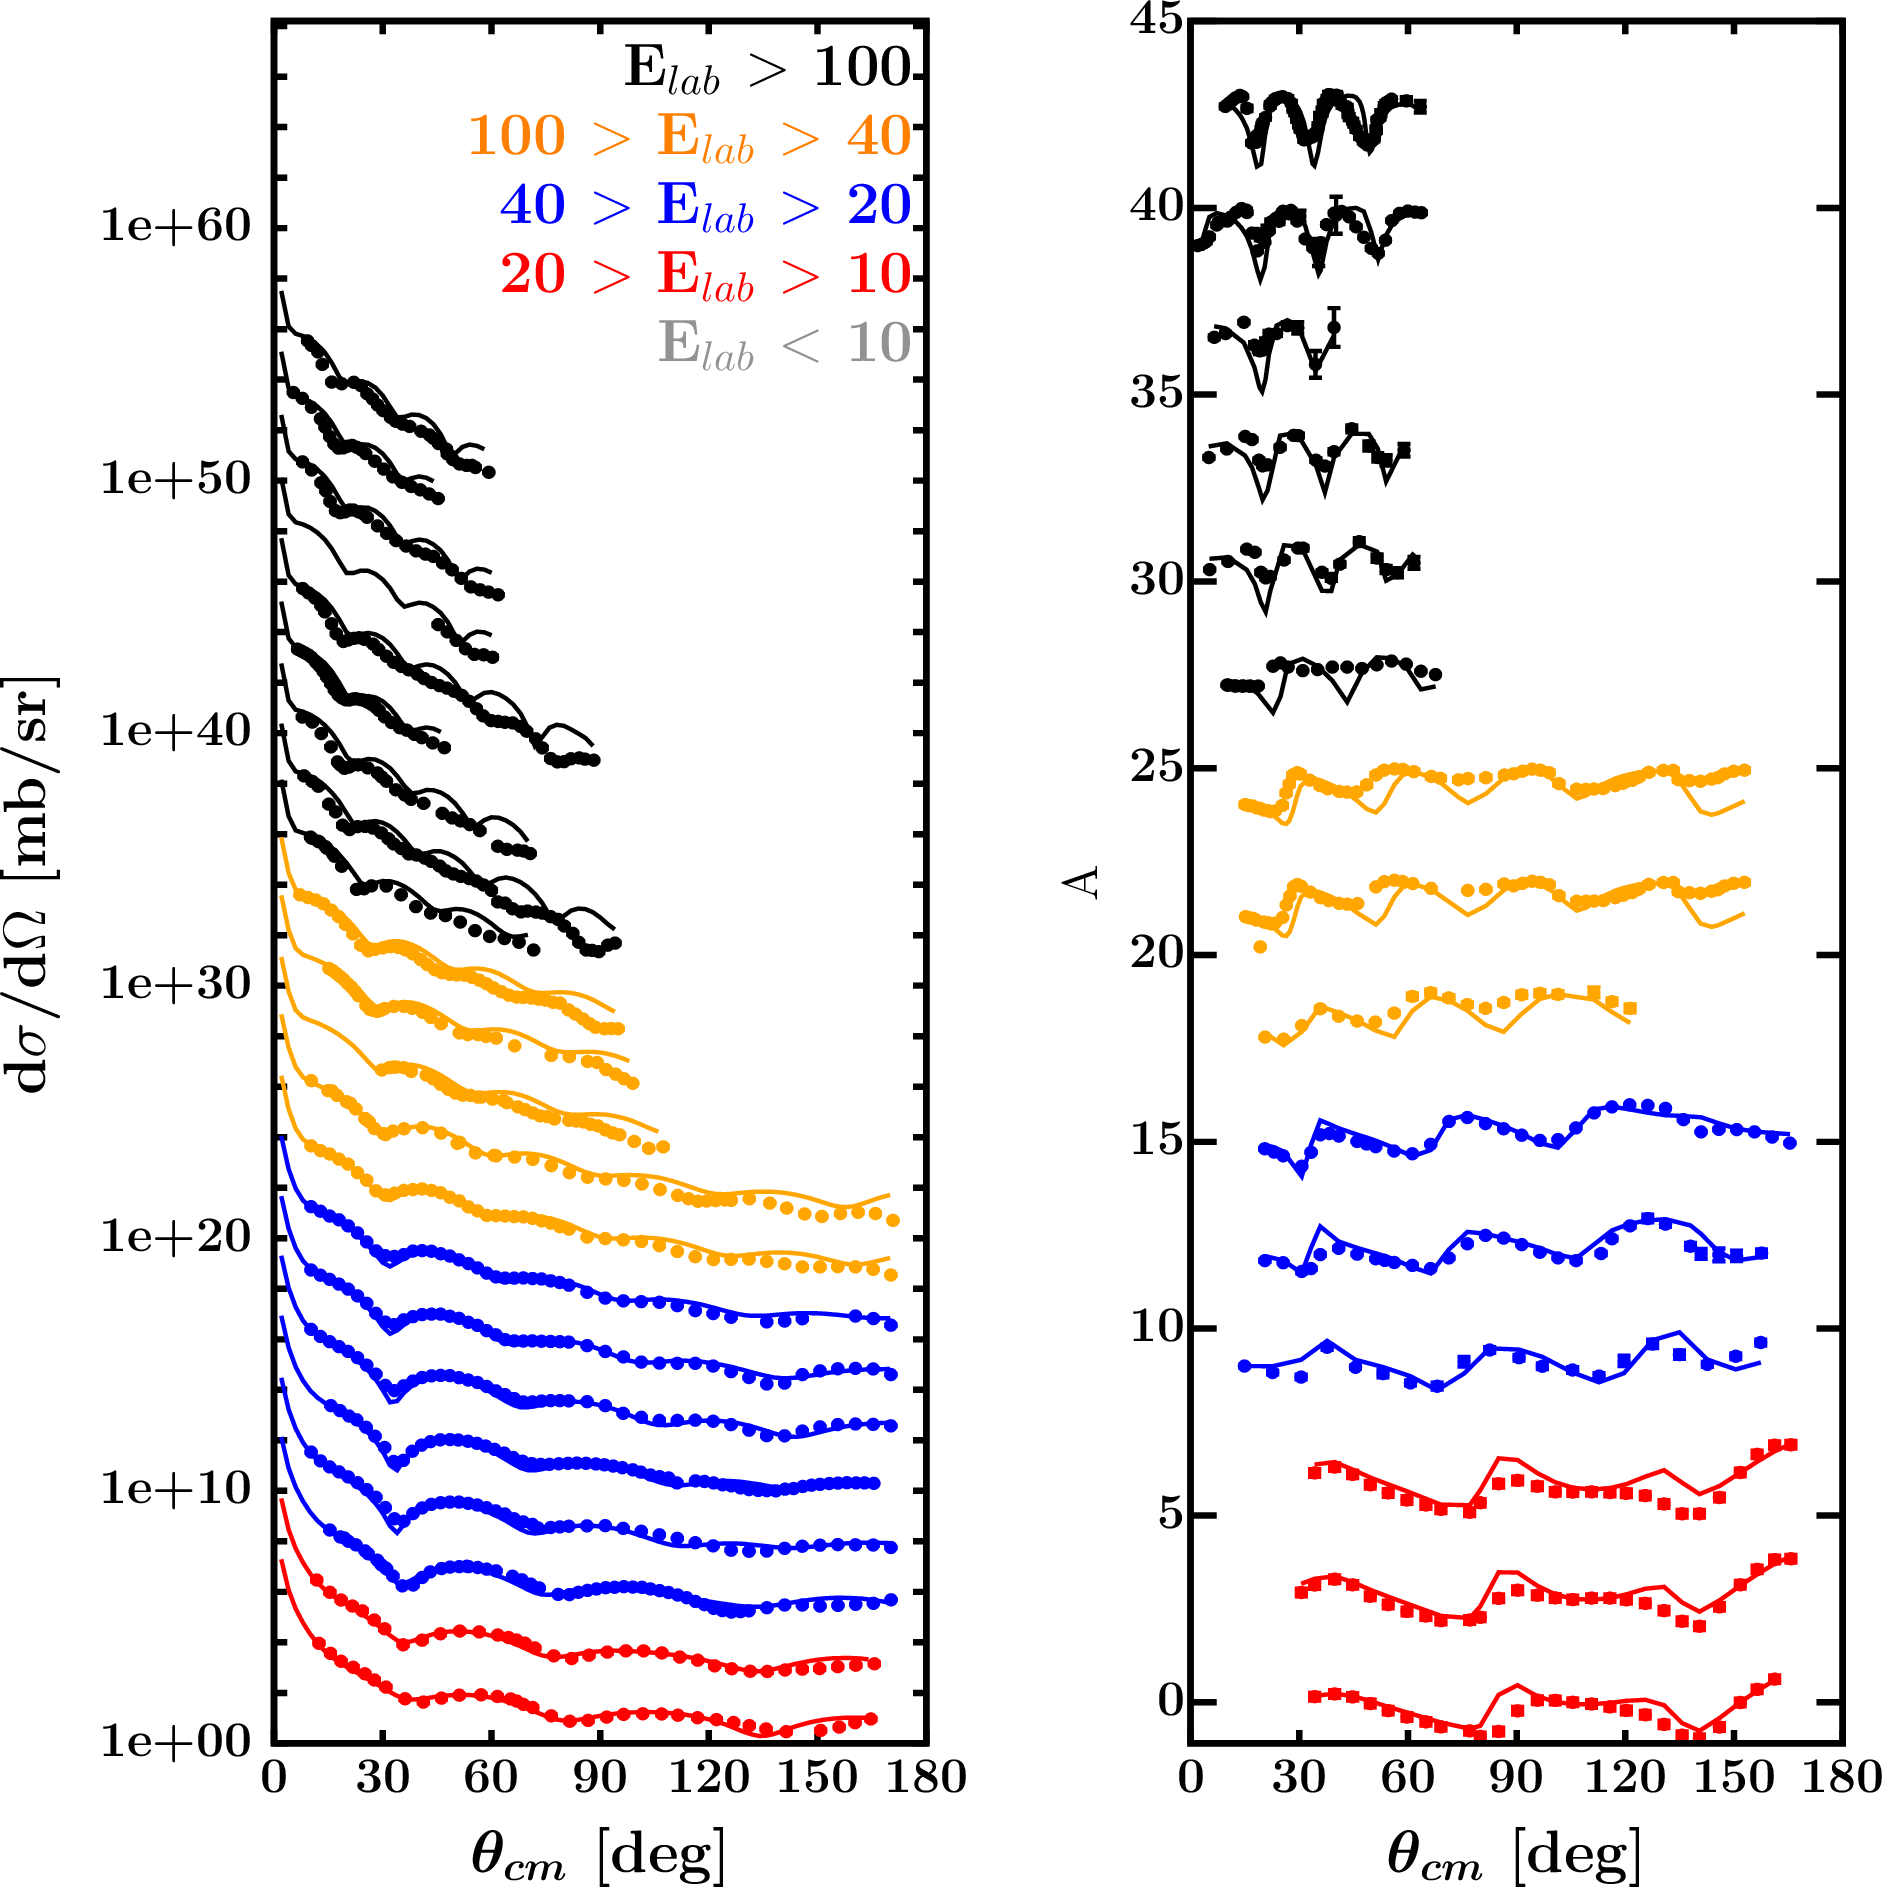
\includegraphics[width=0.85\textwidth]{figures/ca40_protonElastic.png}
    \caption[Proton elastic scattering cross sections on \caForty: DOM predictions and experimental data]
    {
        Proton elastic scattering cross sections on \caForty: experimental data
        and results from DOM fit. Experimental data are shown as points and
        calculated values from the DOM fit of these data are shown as lines.
        Differential cross sections (\el) are shown in the left panel and
        analyzing powers are shown in the right panel. For visual clarity, the 
        data have been offset along the ordinate axis so that the highest-energy data
        appear at the top of the figures. Data are colored according to the
        energy ranges shown in the left panel. References to all experimental data are listed
        in Appendix \ref{DOMDataSets}.
    }
    \label{CaProtonElasticReproduced}
\end{figure}
\begin{figure}[tb]
    \centering
    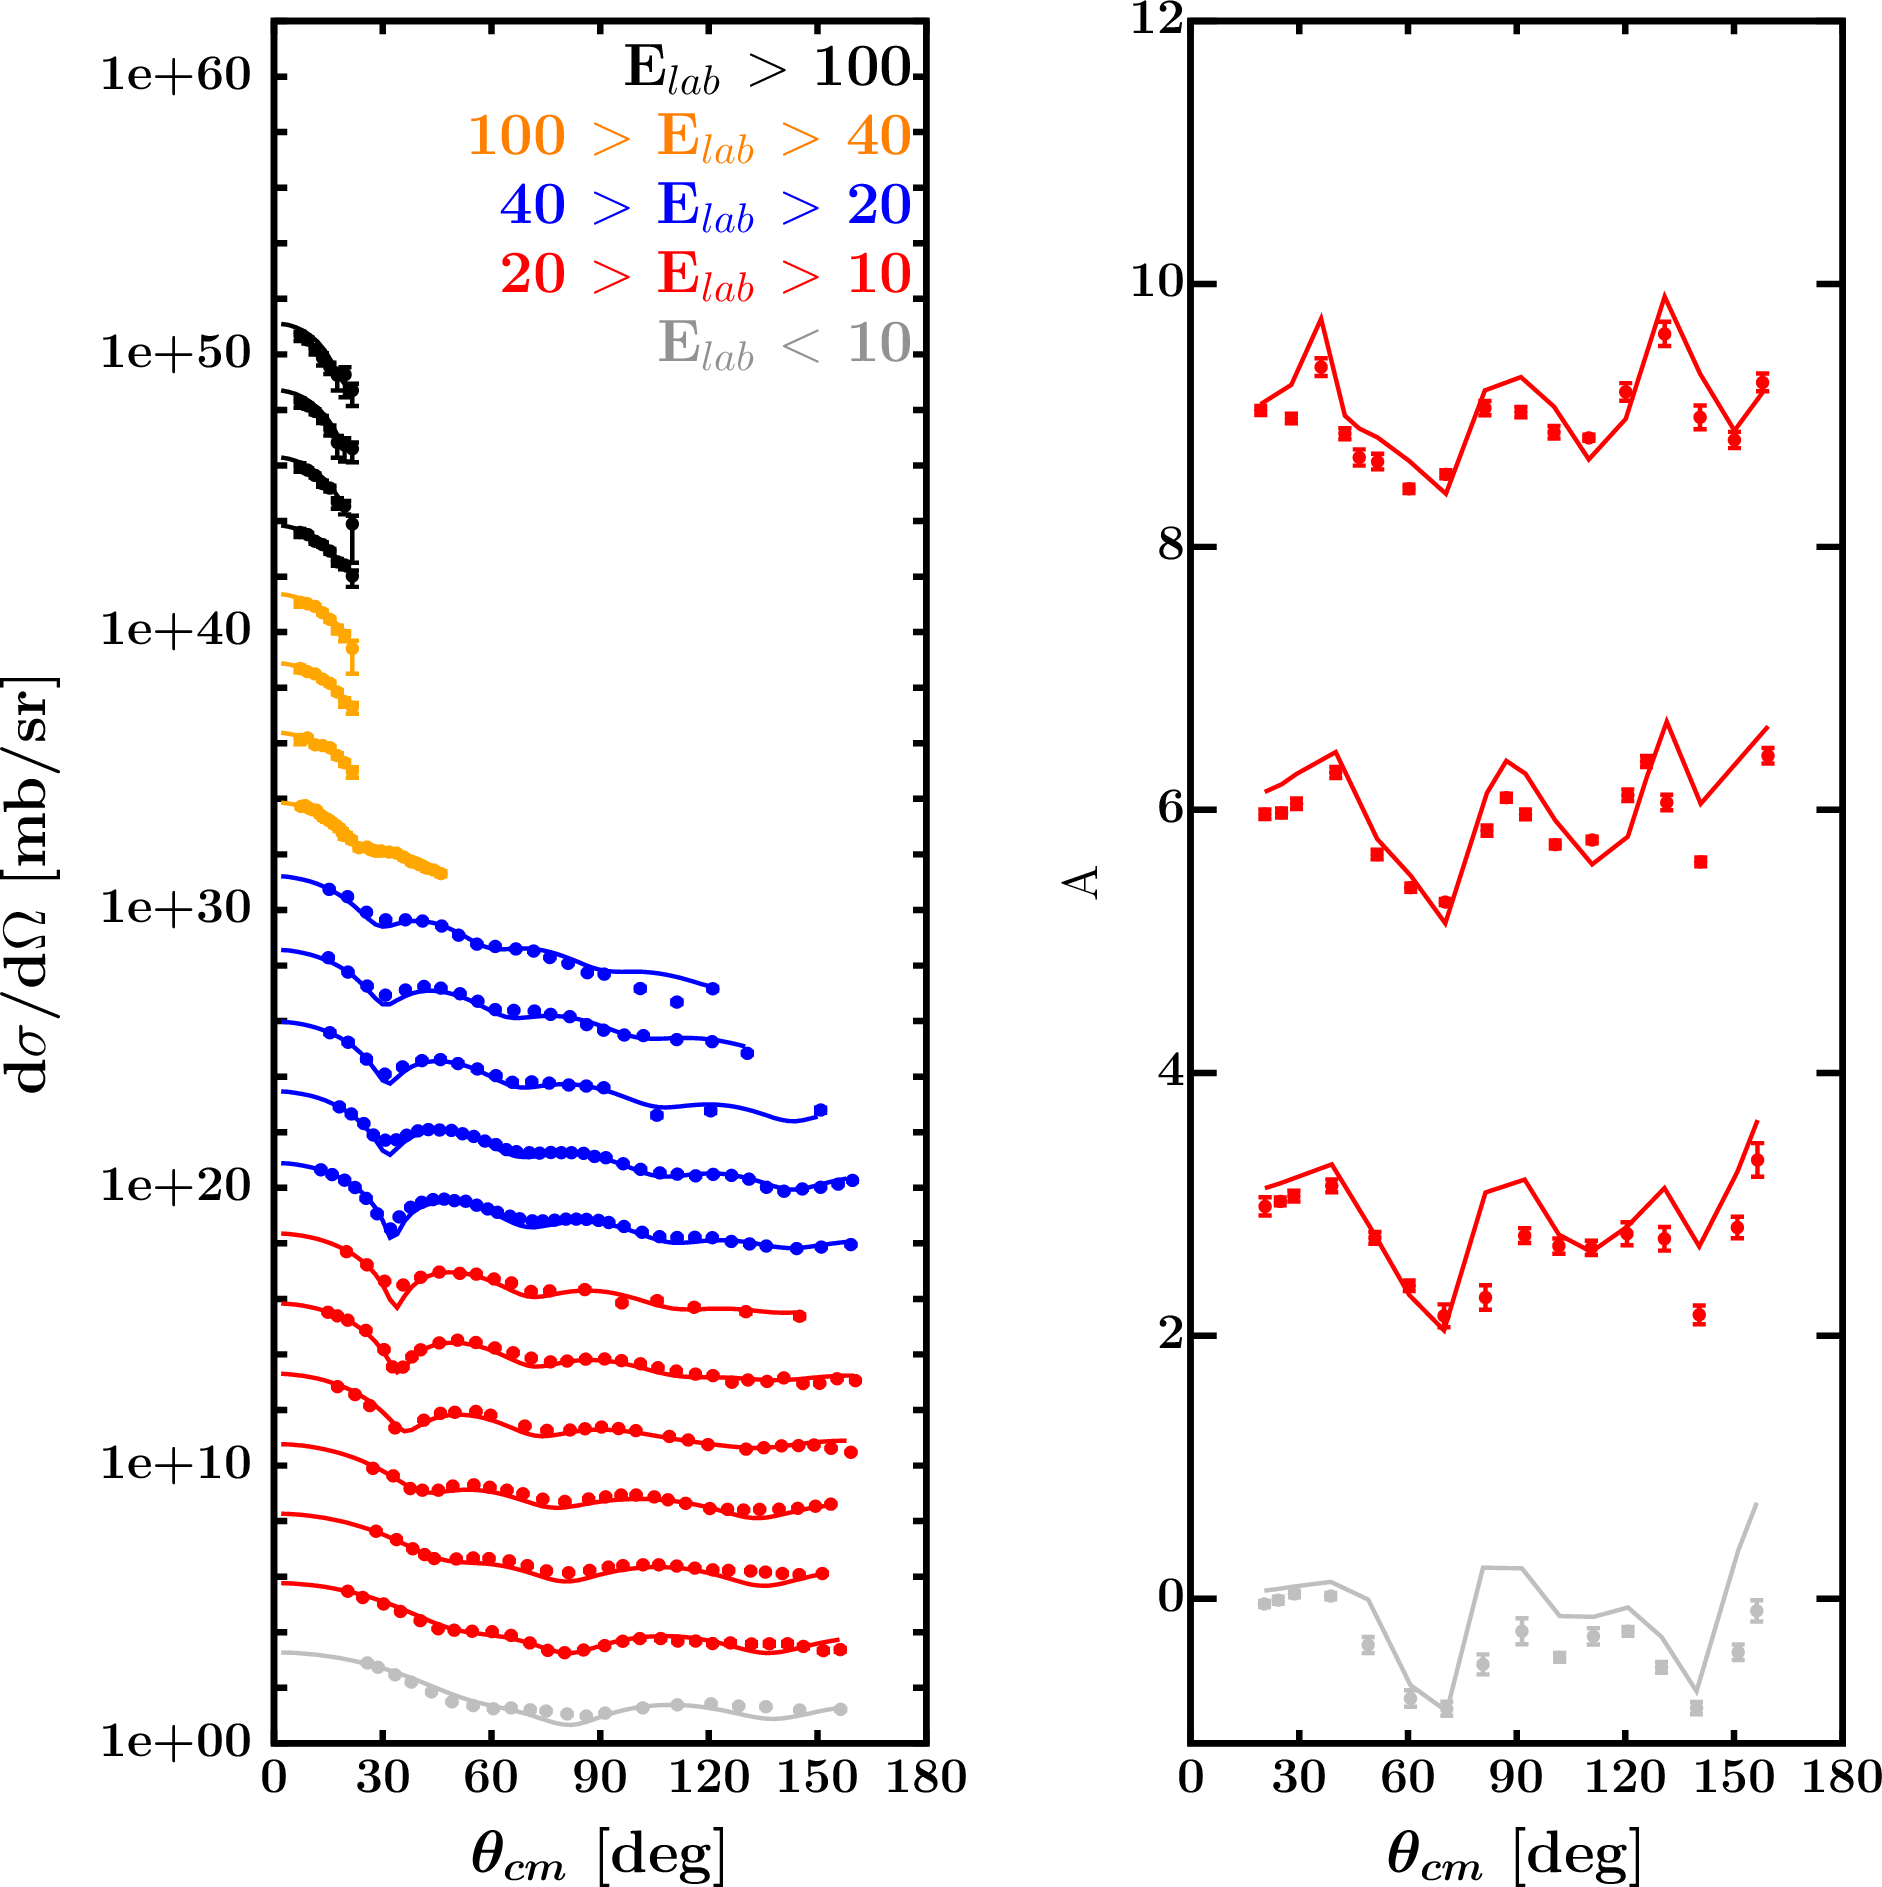
\includegraphics[width=0.85\textwidth]{figures/ca40_neutronElastic.png}
    \caption[Neutron elastic scattering cross sections on \caForty: DOM predictions and experimental data]
    {
        Neutron elastic scattering cross sections on \caForty: experimental data
        and results from DOM fit. Experimental data are shown as points and
        calculated values from the DOM fit of these data are shown as lines.
        Differential cross sections (\el) are shown in the left panel and
        analyzing powers are shown in the right panel. For visual clarity, the 
        data have been offset along the ordinate so that the highest-energy data
        appear at the top of the figures. Data are colored according to the
        energy ranges shown in the left panel. References to all experimental data are listed
        in Appendix \ref{DOMDataSets}.
    }
    \label{CaNeutronElasticReproduced}
\end{figure}

\begin{figure}[tb]
    \centering
    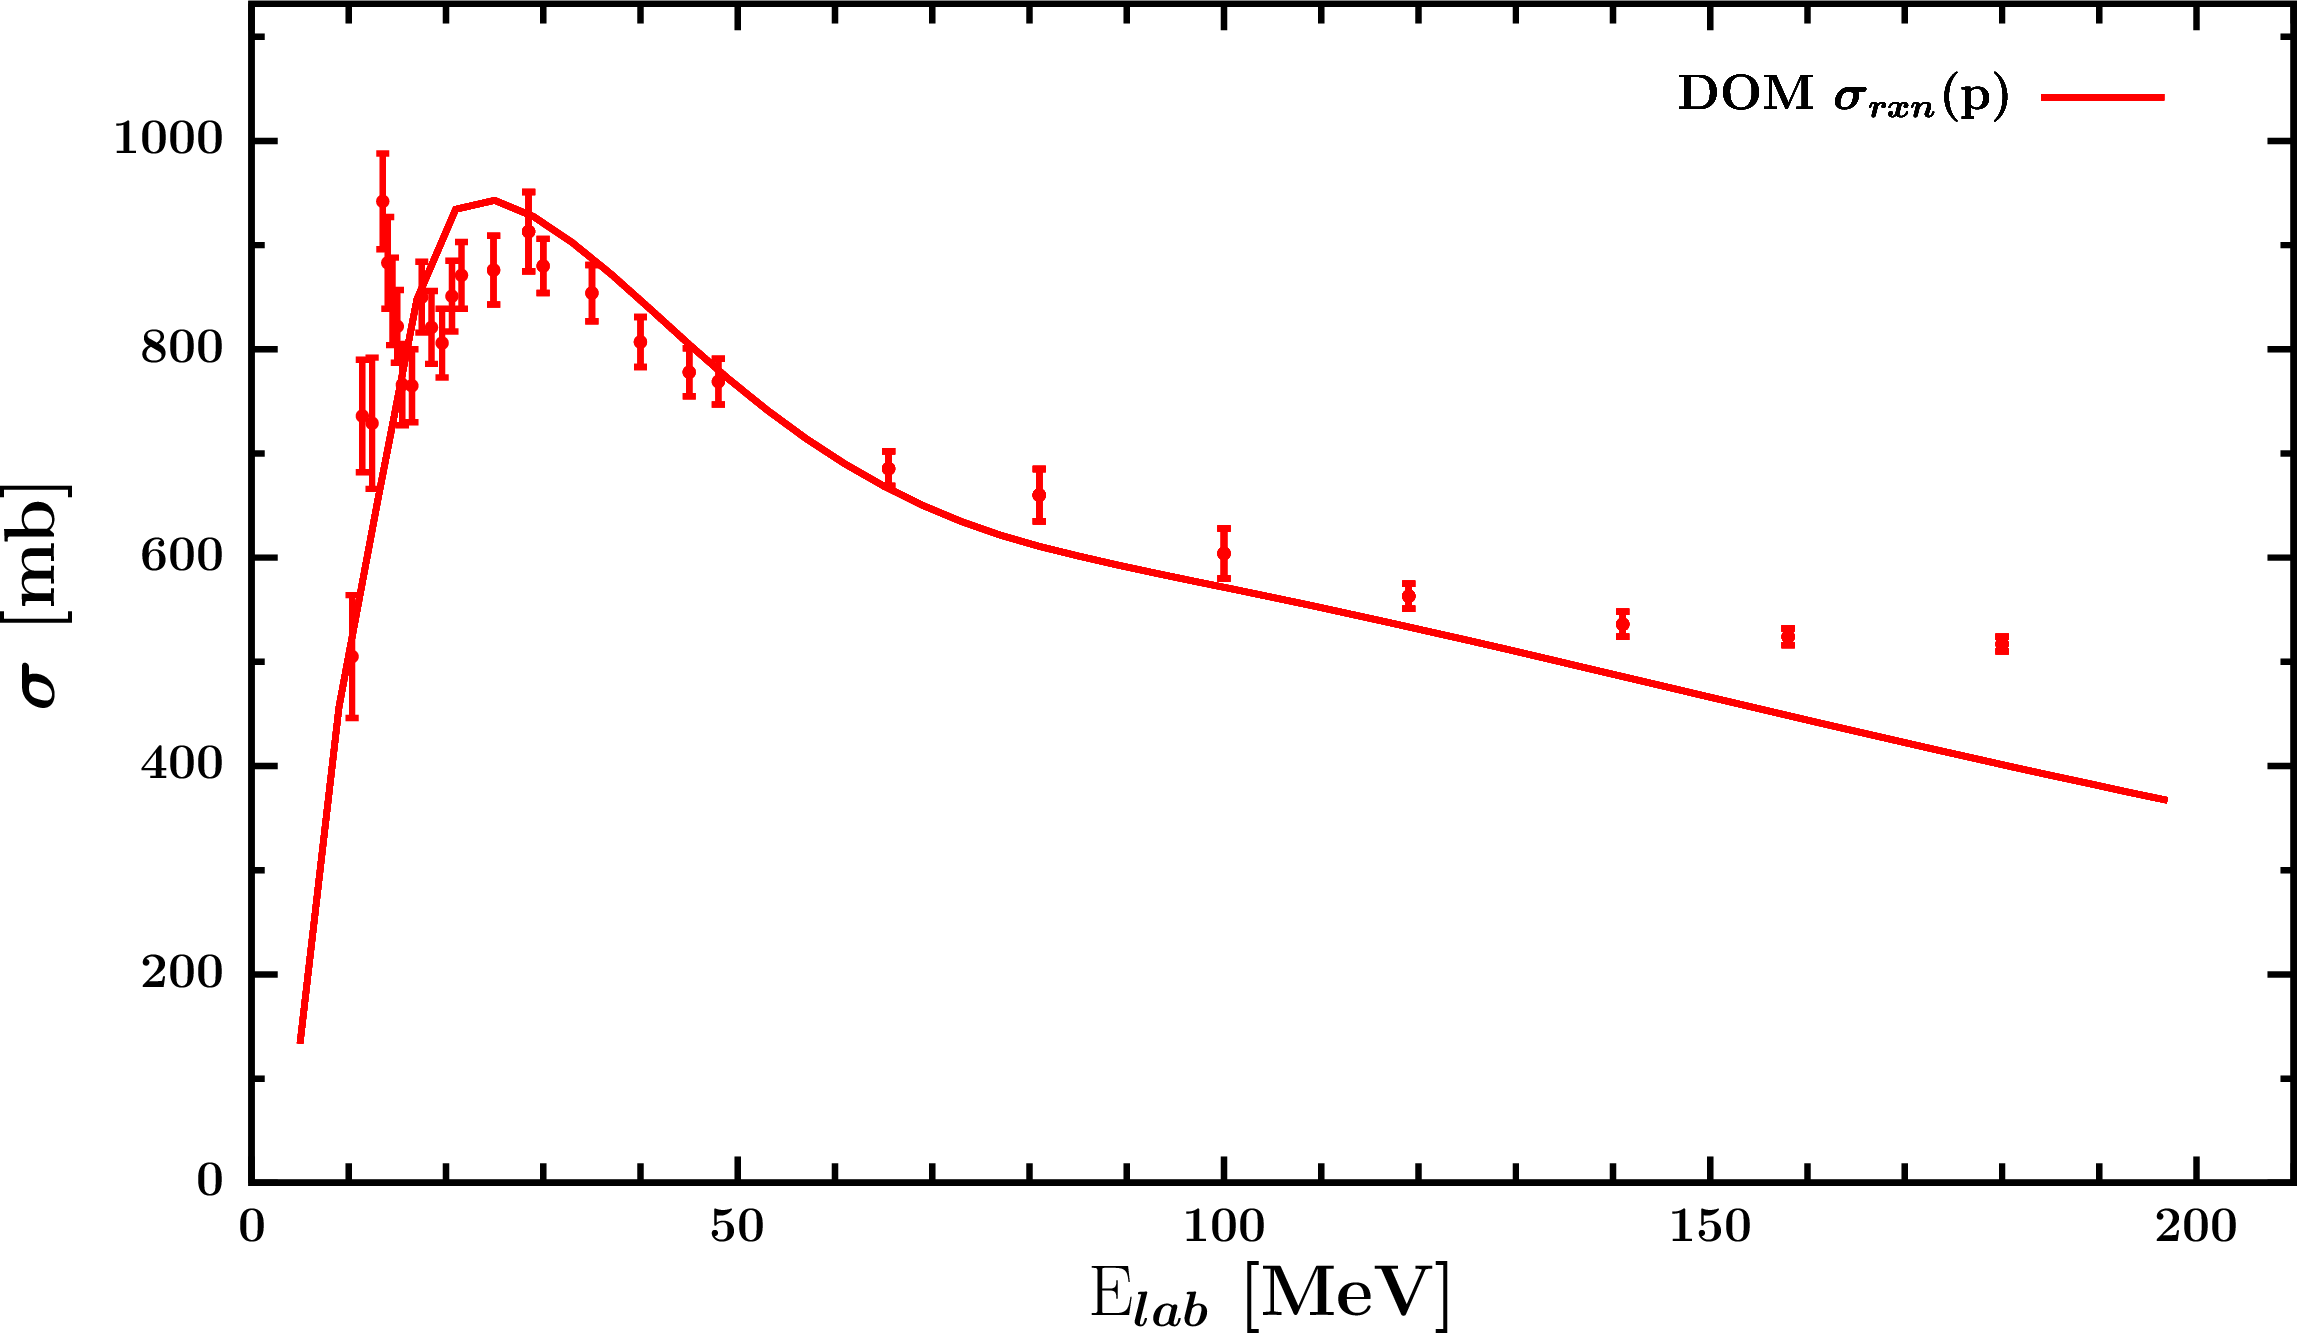
\includegraphics[width=0.82\textwidth]{figures/ca40_protonInelastic.png}
    \caption[Proton \rxn\ of \caForty: DOM predictions and experimental data]
    {
        Proton reaction cross sections on \caForty: experimental data and
        DOM predictions. Experimental data are shown as points and 
        calculated values from our DOM fit of these data are shown
        by the line. References to all experimental
        data are listed in Appendix \ref{DOMDataSets}.
    }
    \label{Ca40ProtonInelastic}
    \vspace{16pt}
    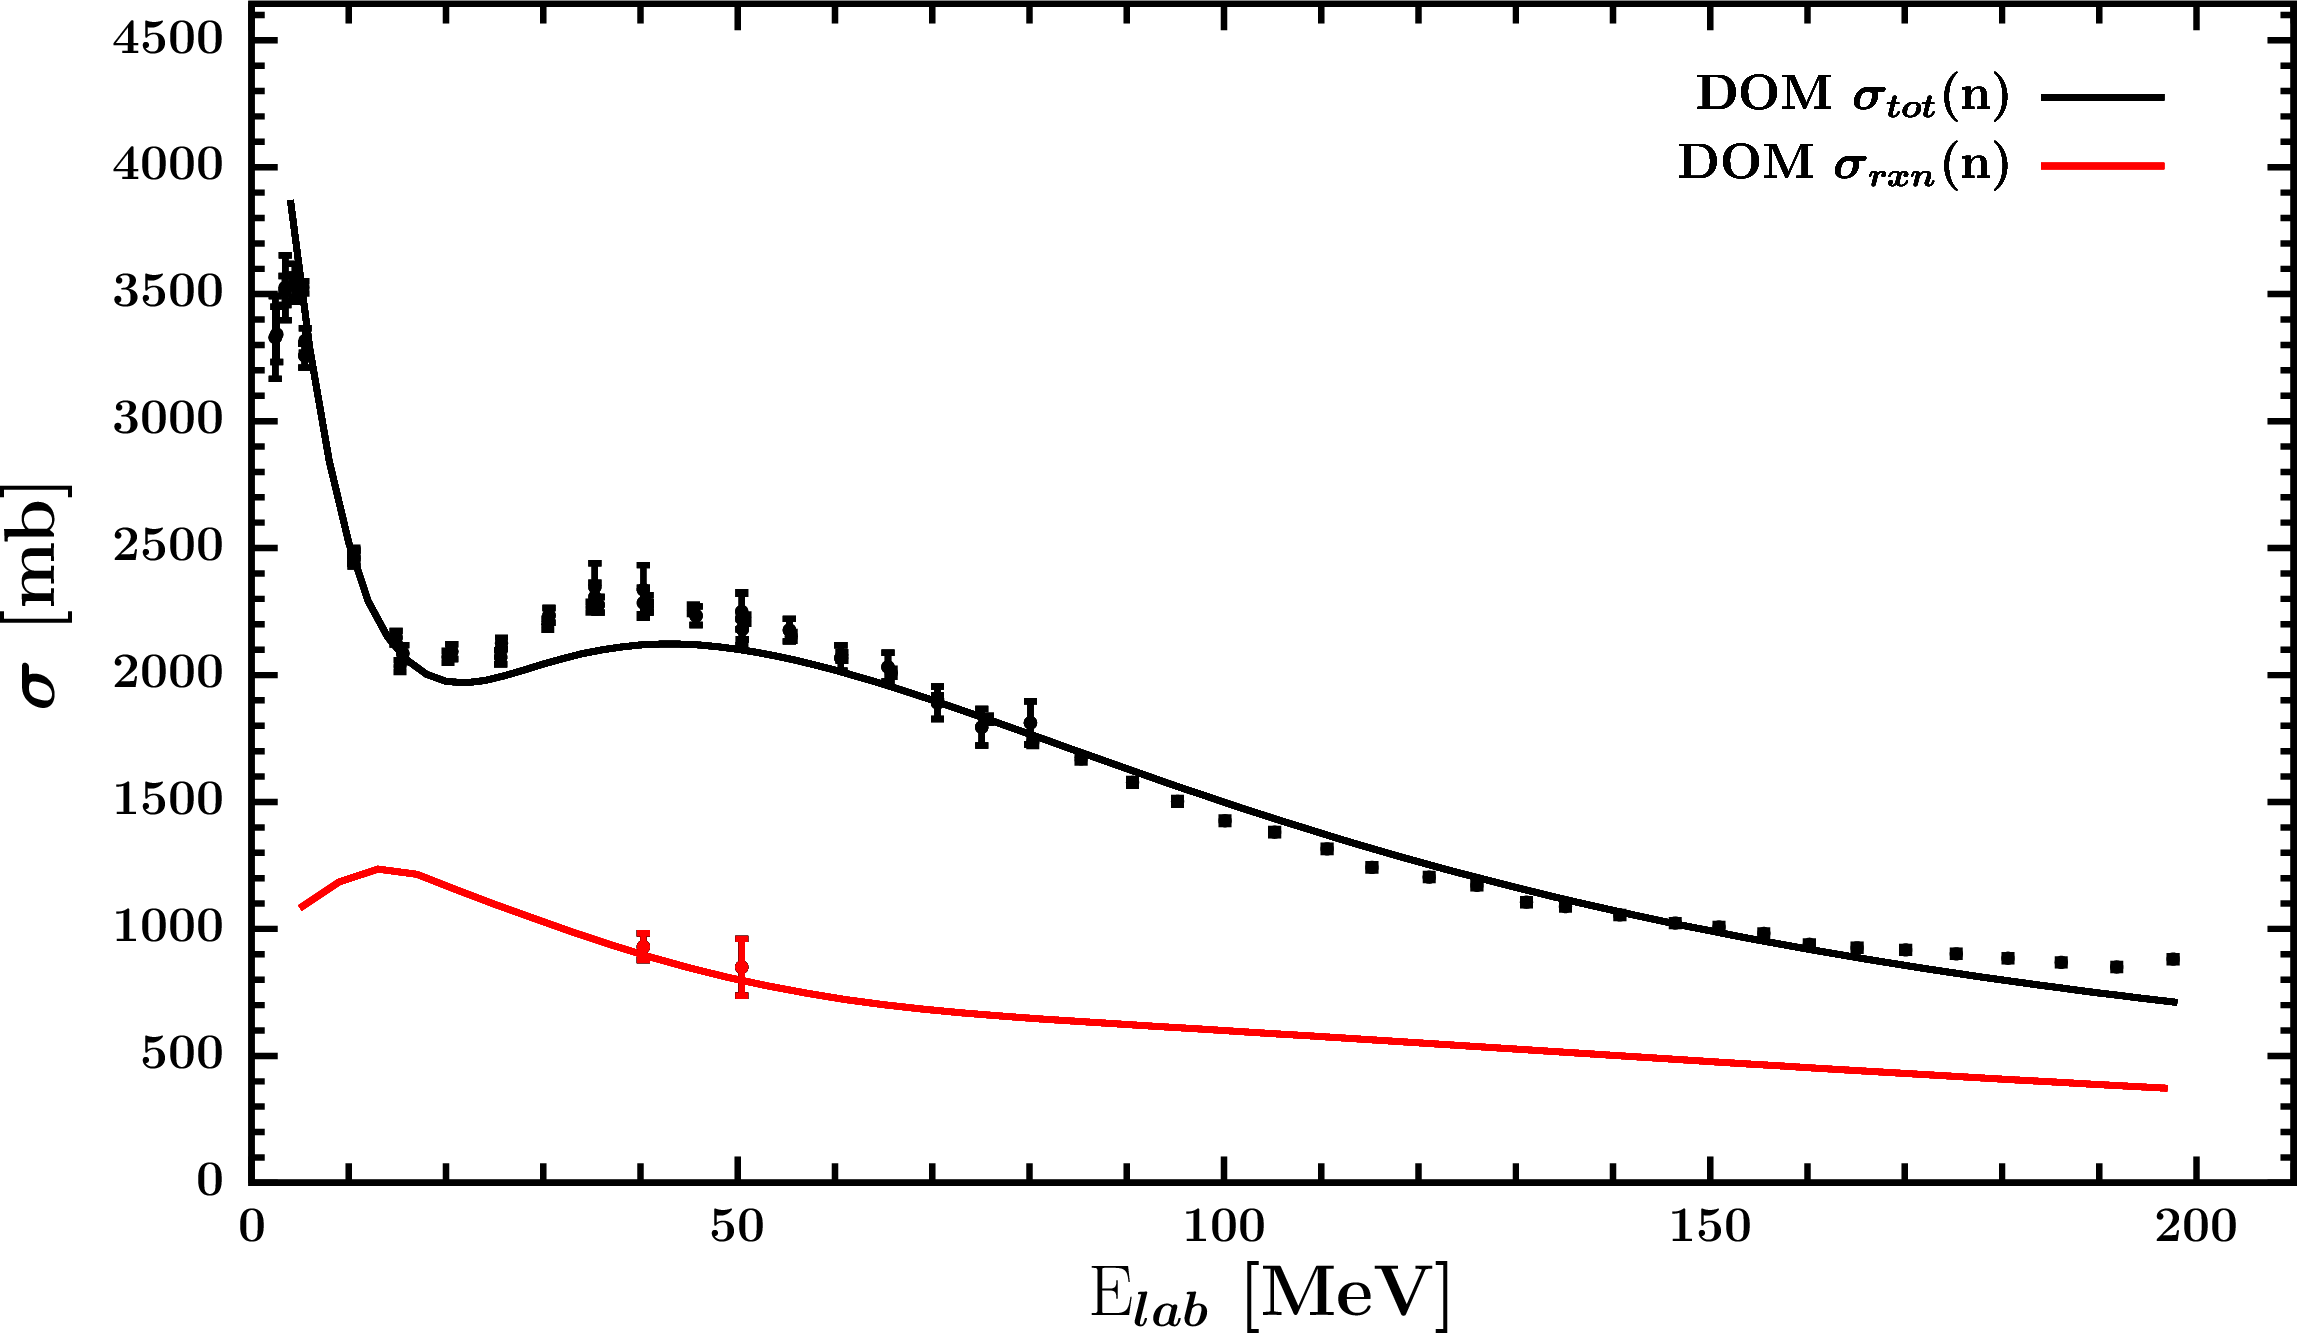
\includegraphics[width=0.82\textwidth]{figures/ca40_neutronInelastic.png}
    \caption[Neutron \rxn\ and \tot\ of \caForty: DOM predictions and experimental data]
    {
        Neutron reaction and total cross sections on \caForty: experimental data and
        DOM predictions. Experimental data are shown as points and 
        calculated values from our DOM fit of these data are shown
        by the line. References to all experimental
        data are listed in Appendix \ref{DOMDataSets}.
    }
    \label{Ca40NeutronInelastic}
\end{figure}

\begin{figure}[tb]
    \centering
    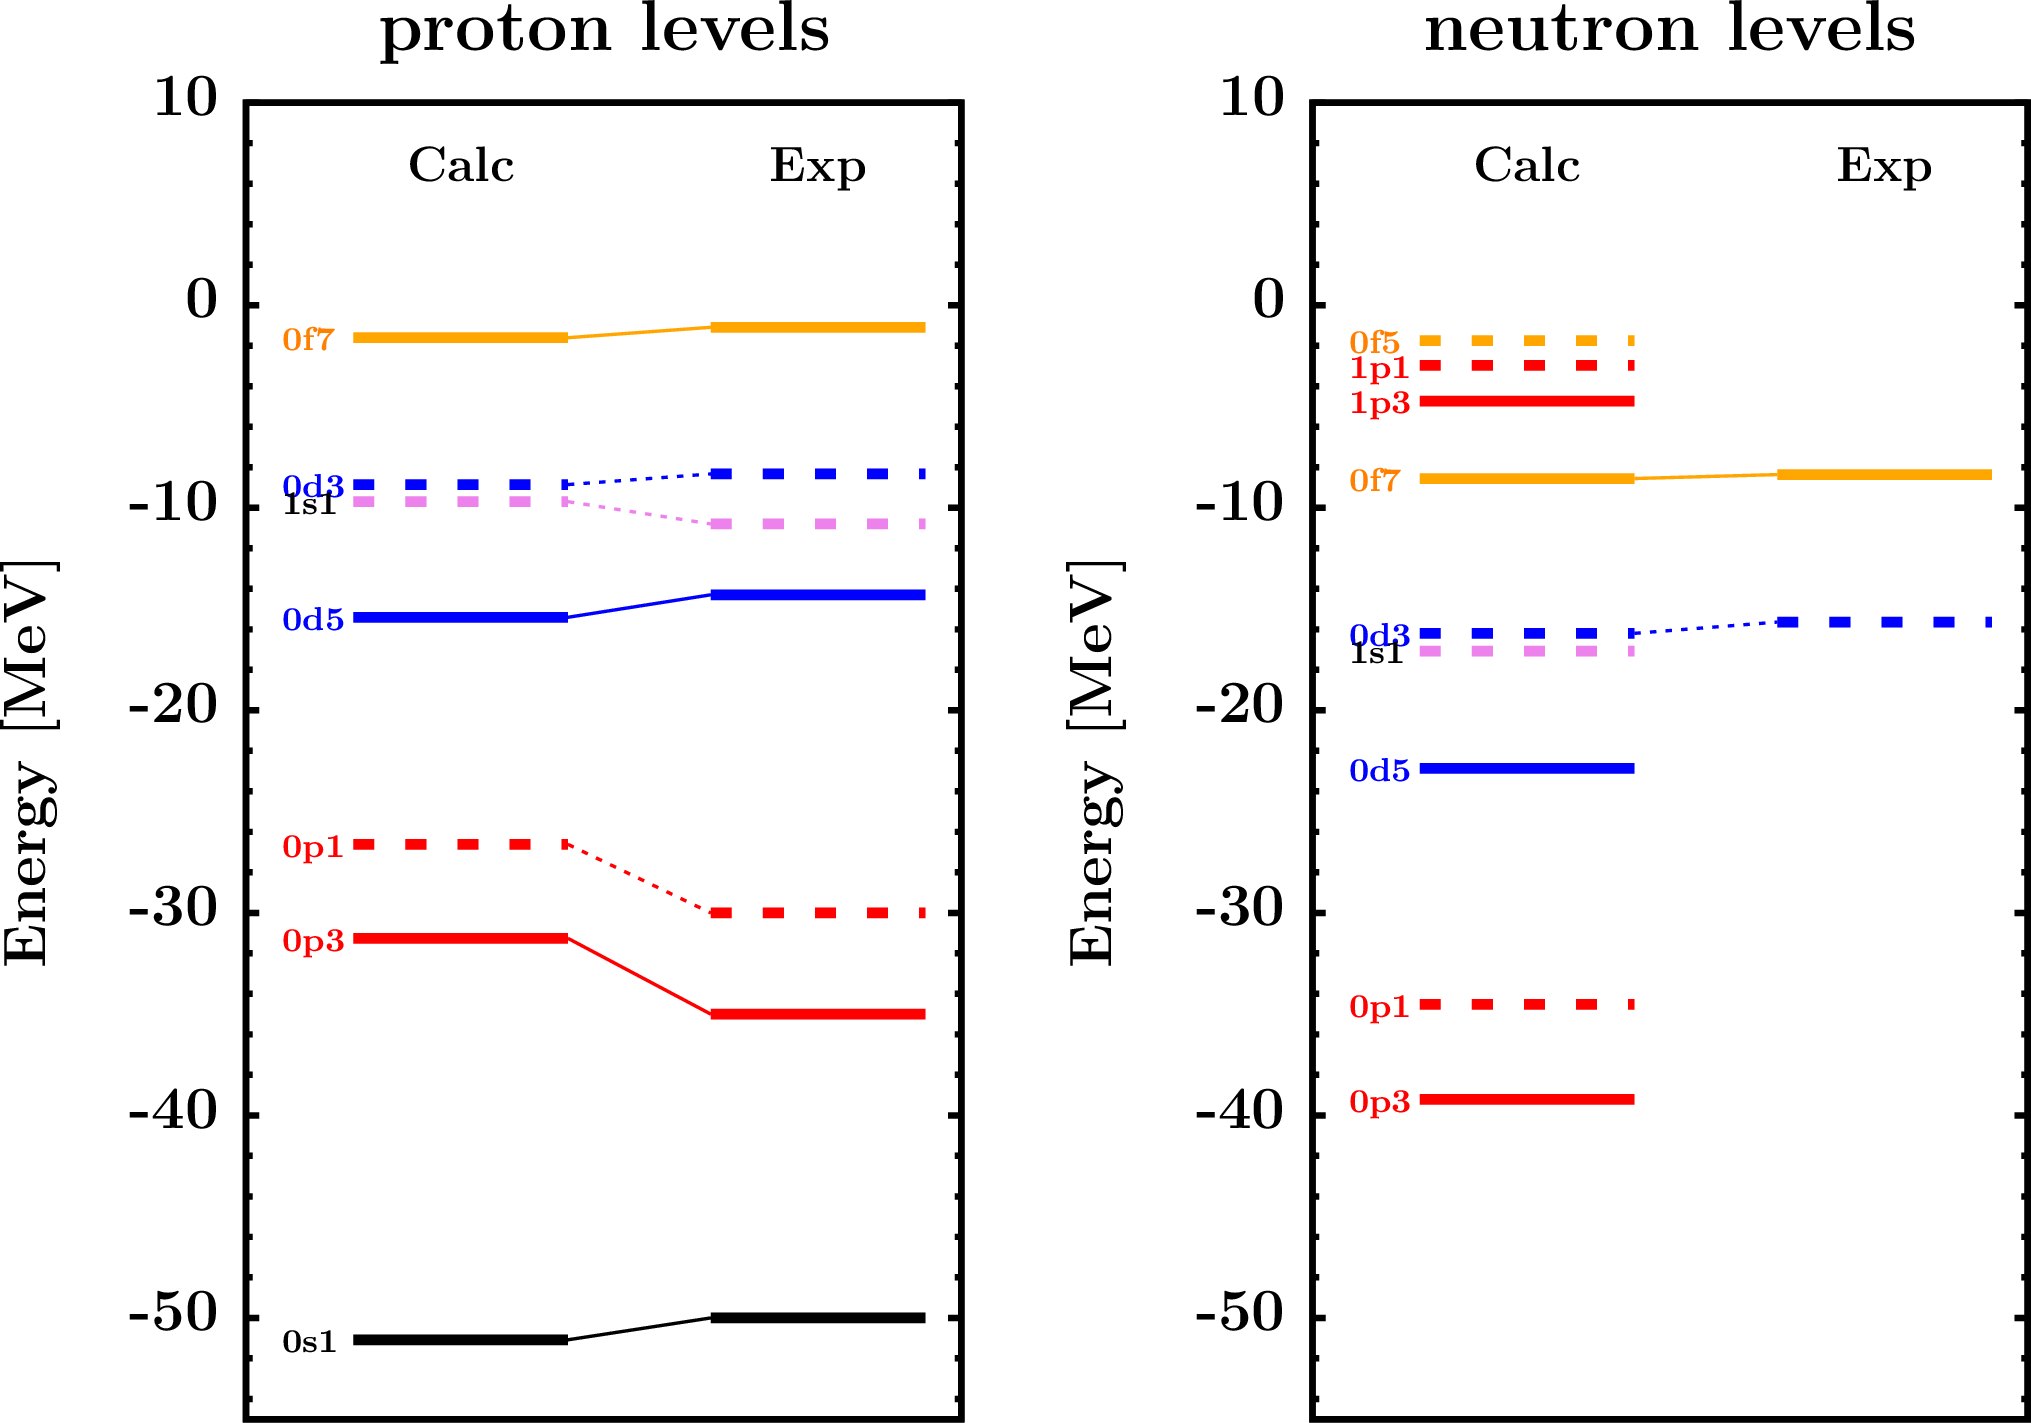
\includegraphics[width=\textwidth]{figures/ca40_SPLevels.png}
    \caption[Single-particle levels in \caForty]
    {
        Single-particle energy levels in \caForty\ for protons and neutrons.
        In each panel, calculated energies are shown on the left and
        experimental energies are shown on the right. References to all
        experimental data used to estimate these energy levels are
        listed in Appendix \ref{DOMDataSets}.
    }
    \label{Ca40SPLevels}
\end{figure}

\begin{figure}[tb]
    \centering
    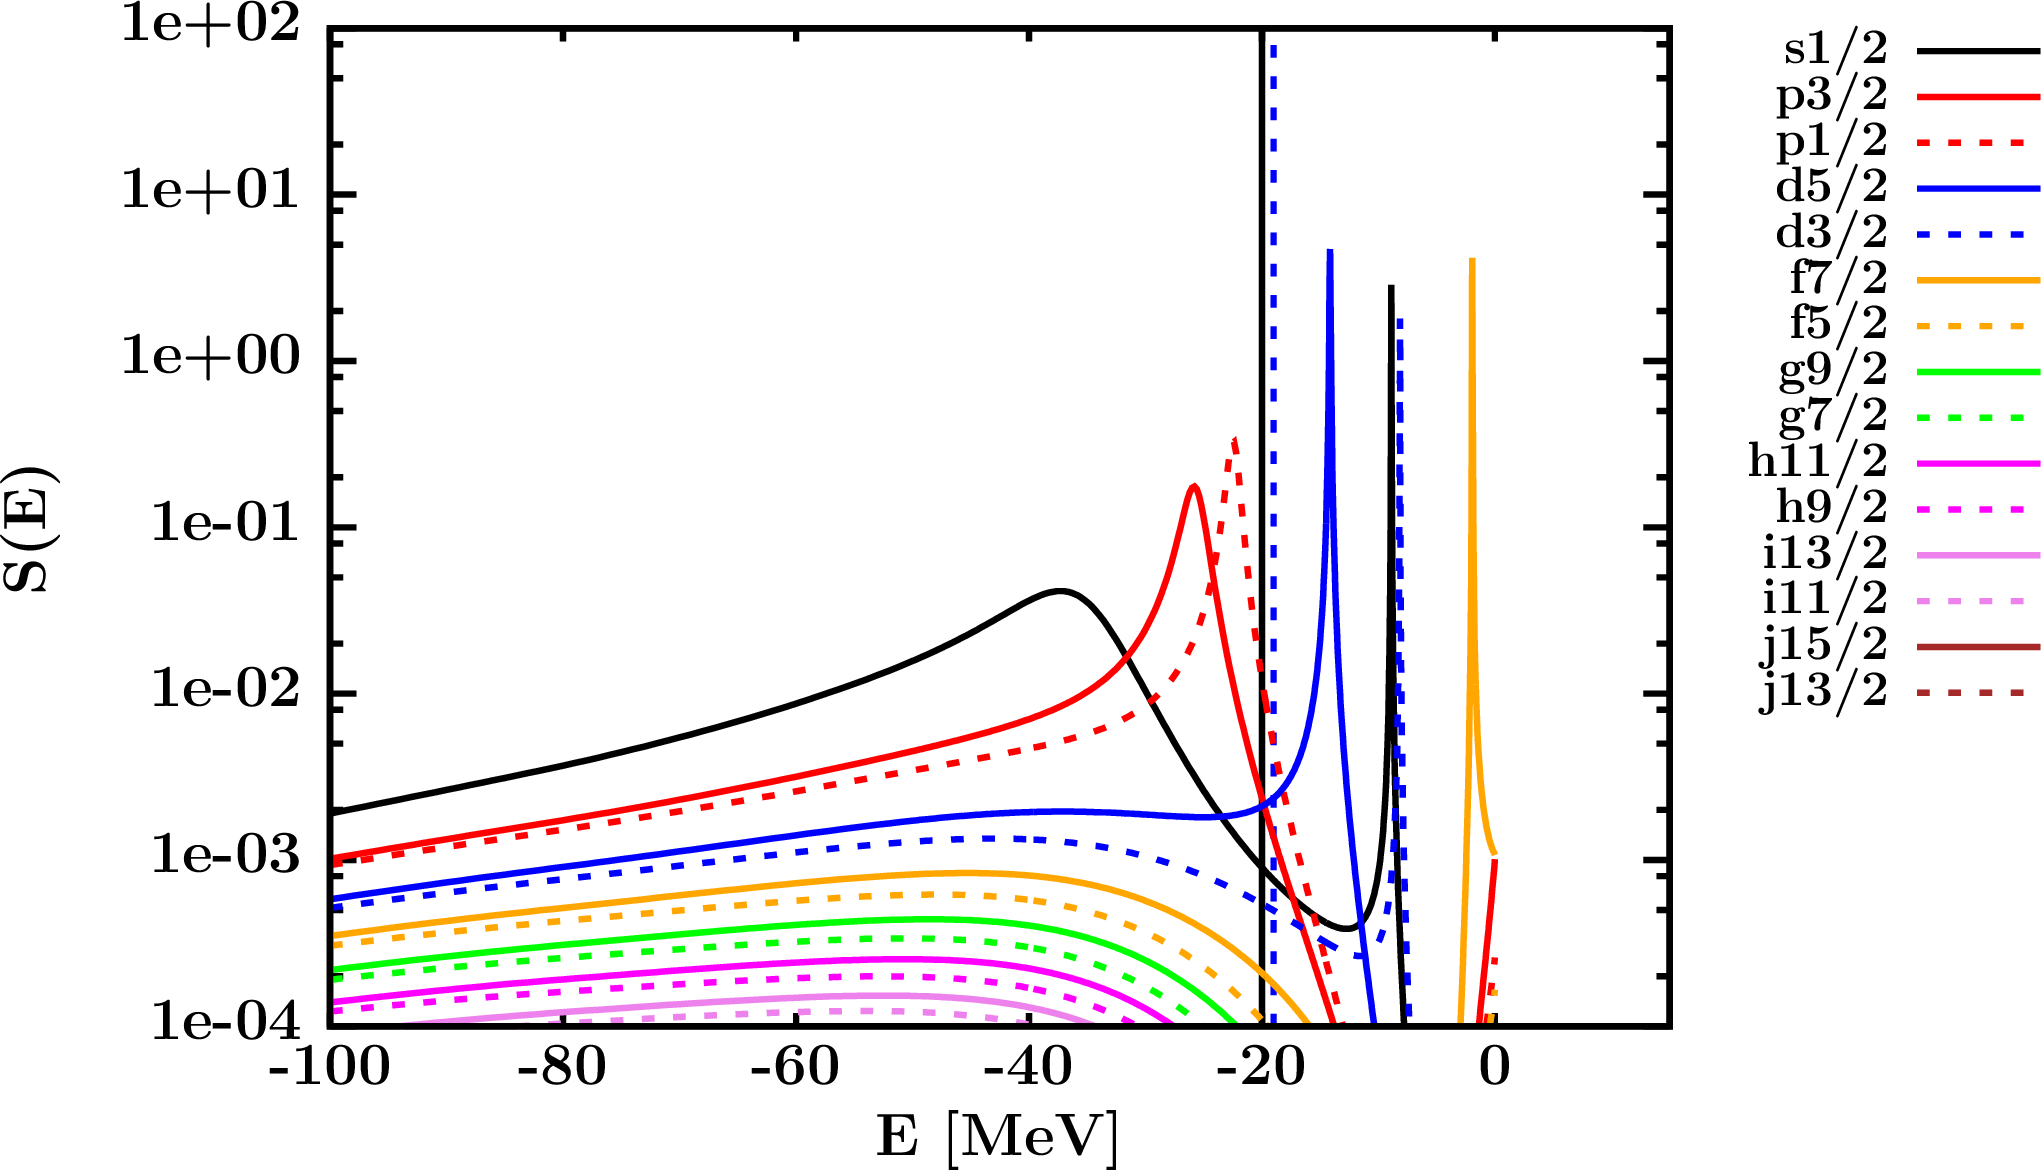
\includegraphics[width=\textwidth]{figures/ca40_protonSpectralFunctions.png}
    \caption[Proton spectral functions in \caForty]
    {
        Proton spectral functions by orbital angular momentum $L$ and total
        angular momentum $J$ in \caForty, as generated by our DOM fit.
        In deeply-bound shells,
        spectral peak broadening is obvious, a consequence of increased
        imaginary strength in the self-energy at energies far from the
        Fermi energy. The shape and location of the \textit{neutron} spectral
        functions in \caForty\ are similar except for a Coulomb shift. The
        general shape and degree of occupation depletion associated with our spectral
        functions agree with results of (p,2p) and (e,e'p) scattering
        and former DOM treatments \cite{MahzoonPhDThesis}.
    }
    \label{Ca40SpectralFunctions}
\end{figure}

\begin{figure}[tb]
    \centering
    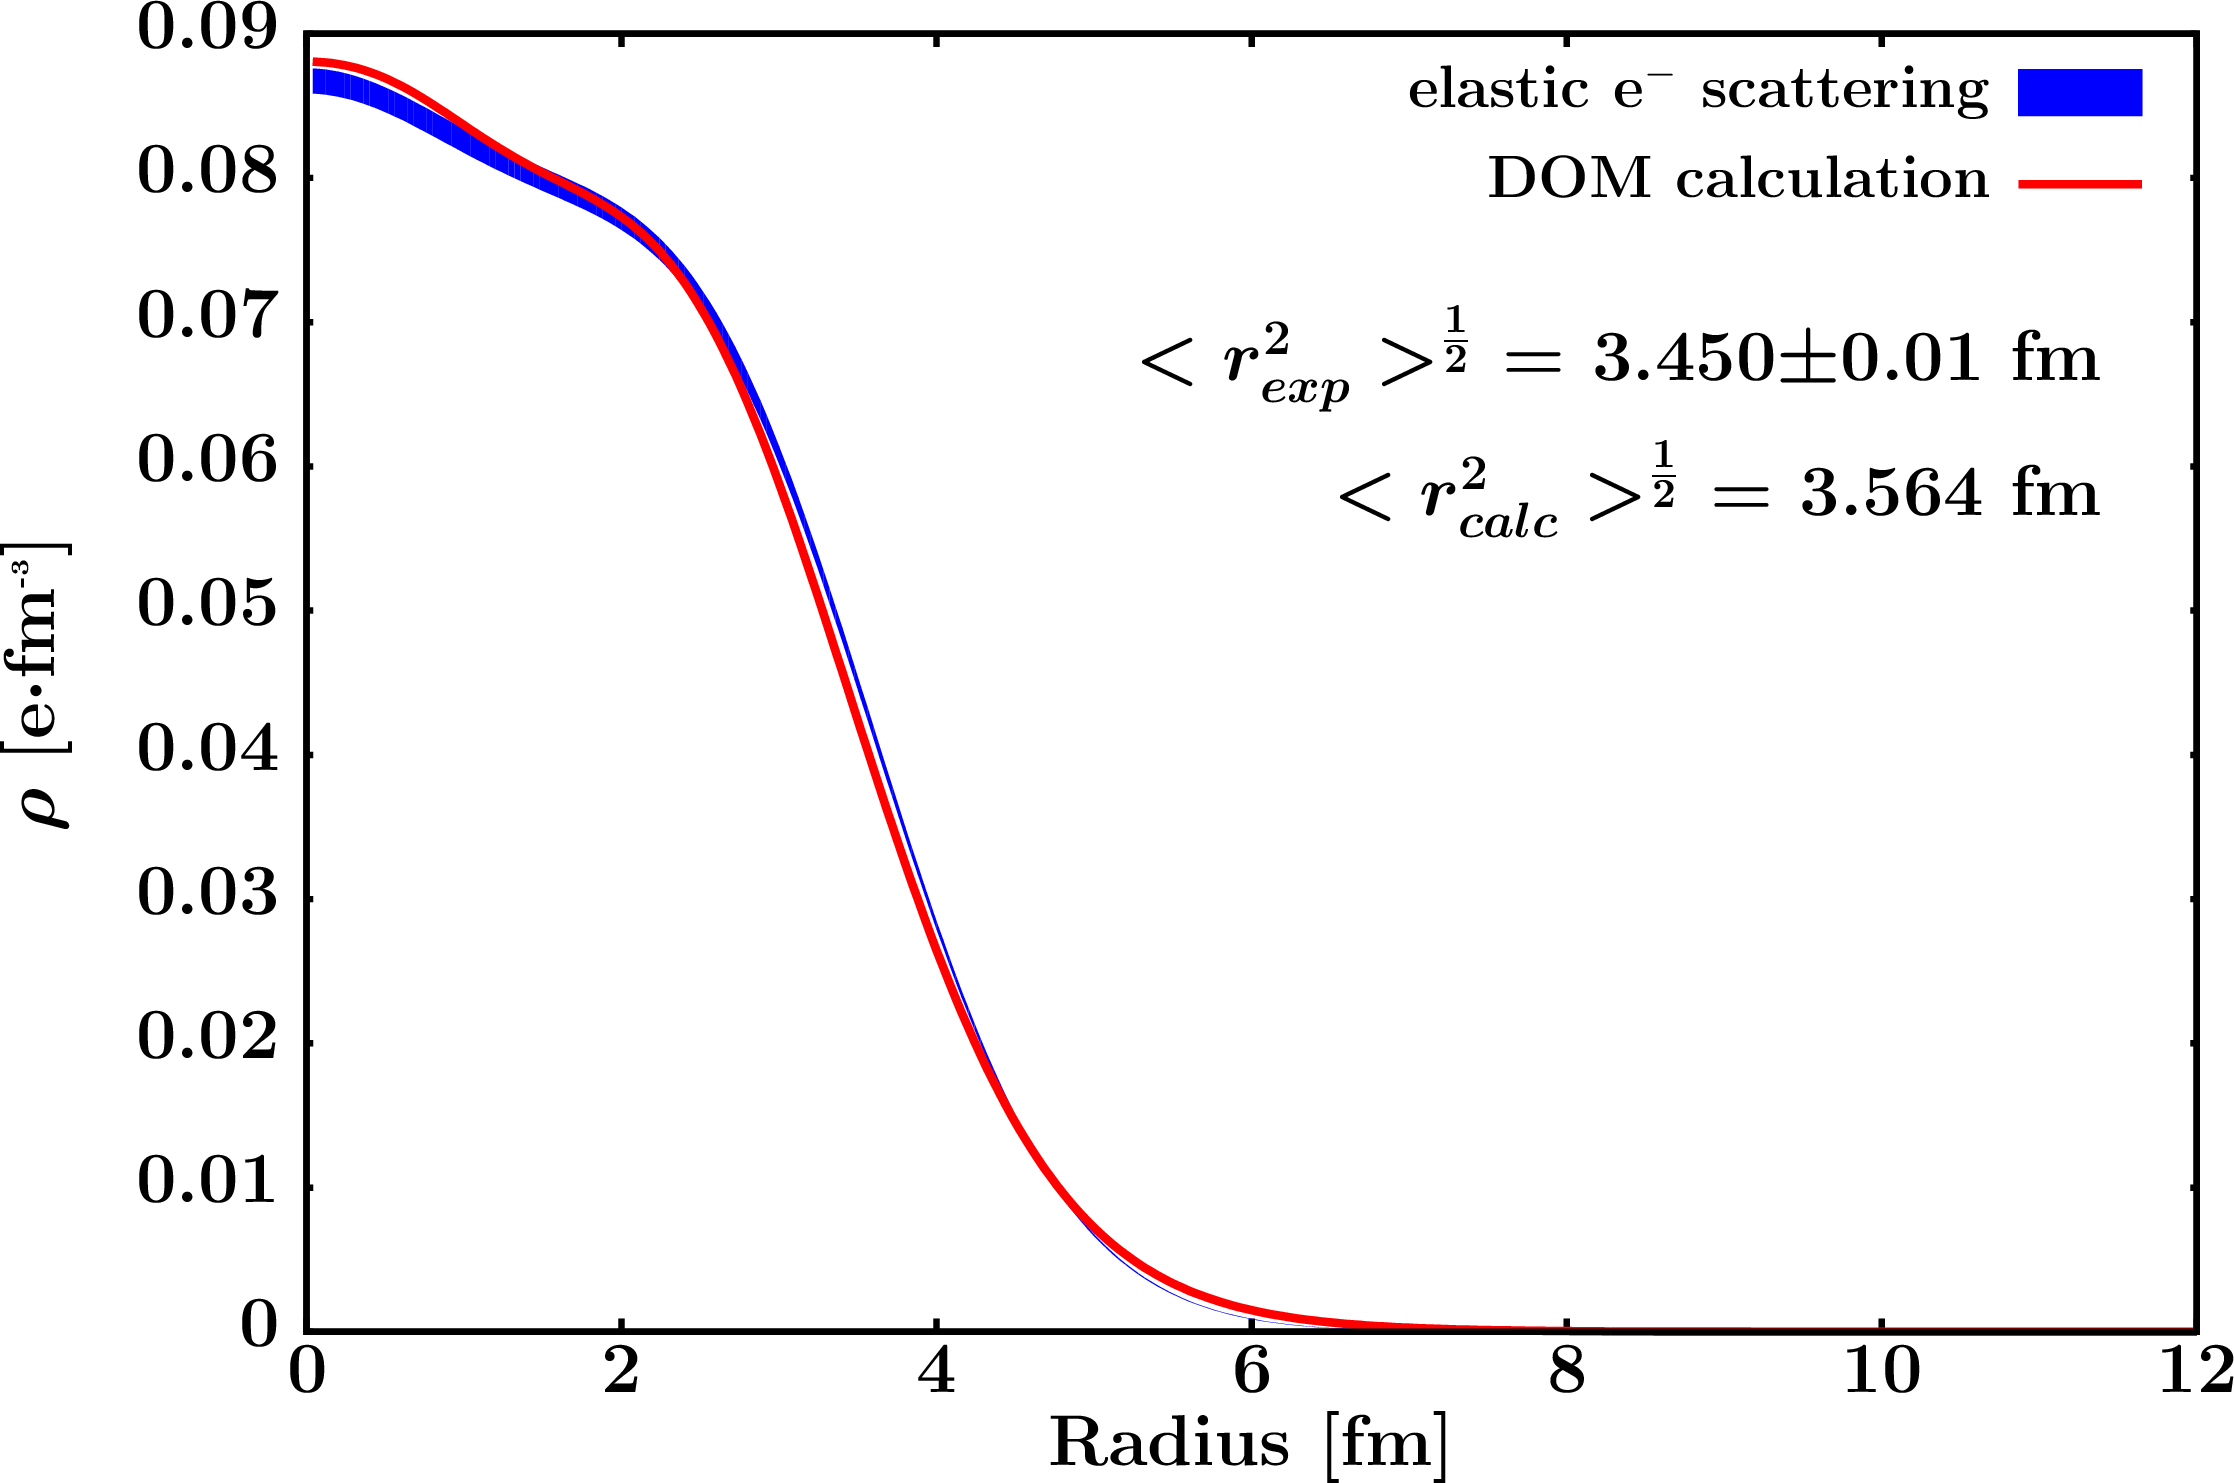
\includegraphics[width=0.75\textwidth]{figures/ca40_chargeDensity.png}
    \caption[Proton single-particle density distributions in \caForty]
    {
        Charge density distribution of \caForty, as generated
        by our DOM fit (in red) and as generated from experimental
        elastic electron scattering \cite{DeVries1987}. No error bars are
        reported in the compilation of \cite{DeVries1987}; we show an
        arbitrary uncertainty range of 1\% (blue shaded region).
    }
    \label{Ca40ChargeDensity}
    \vspace{16pt}
    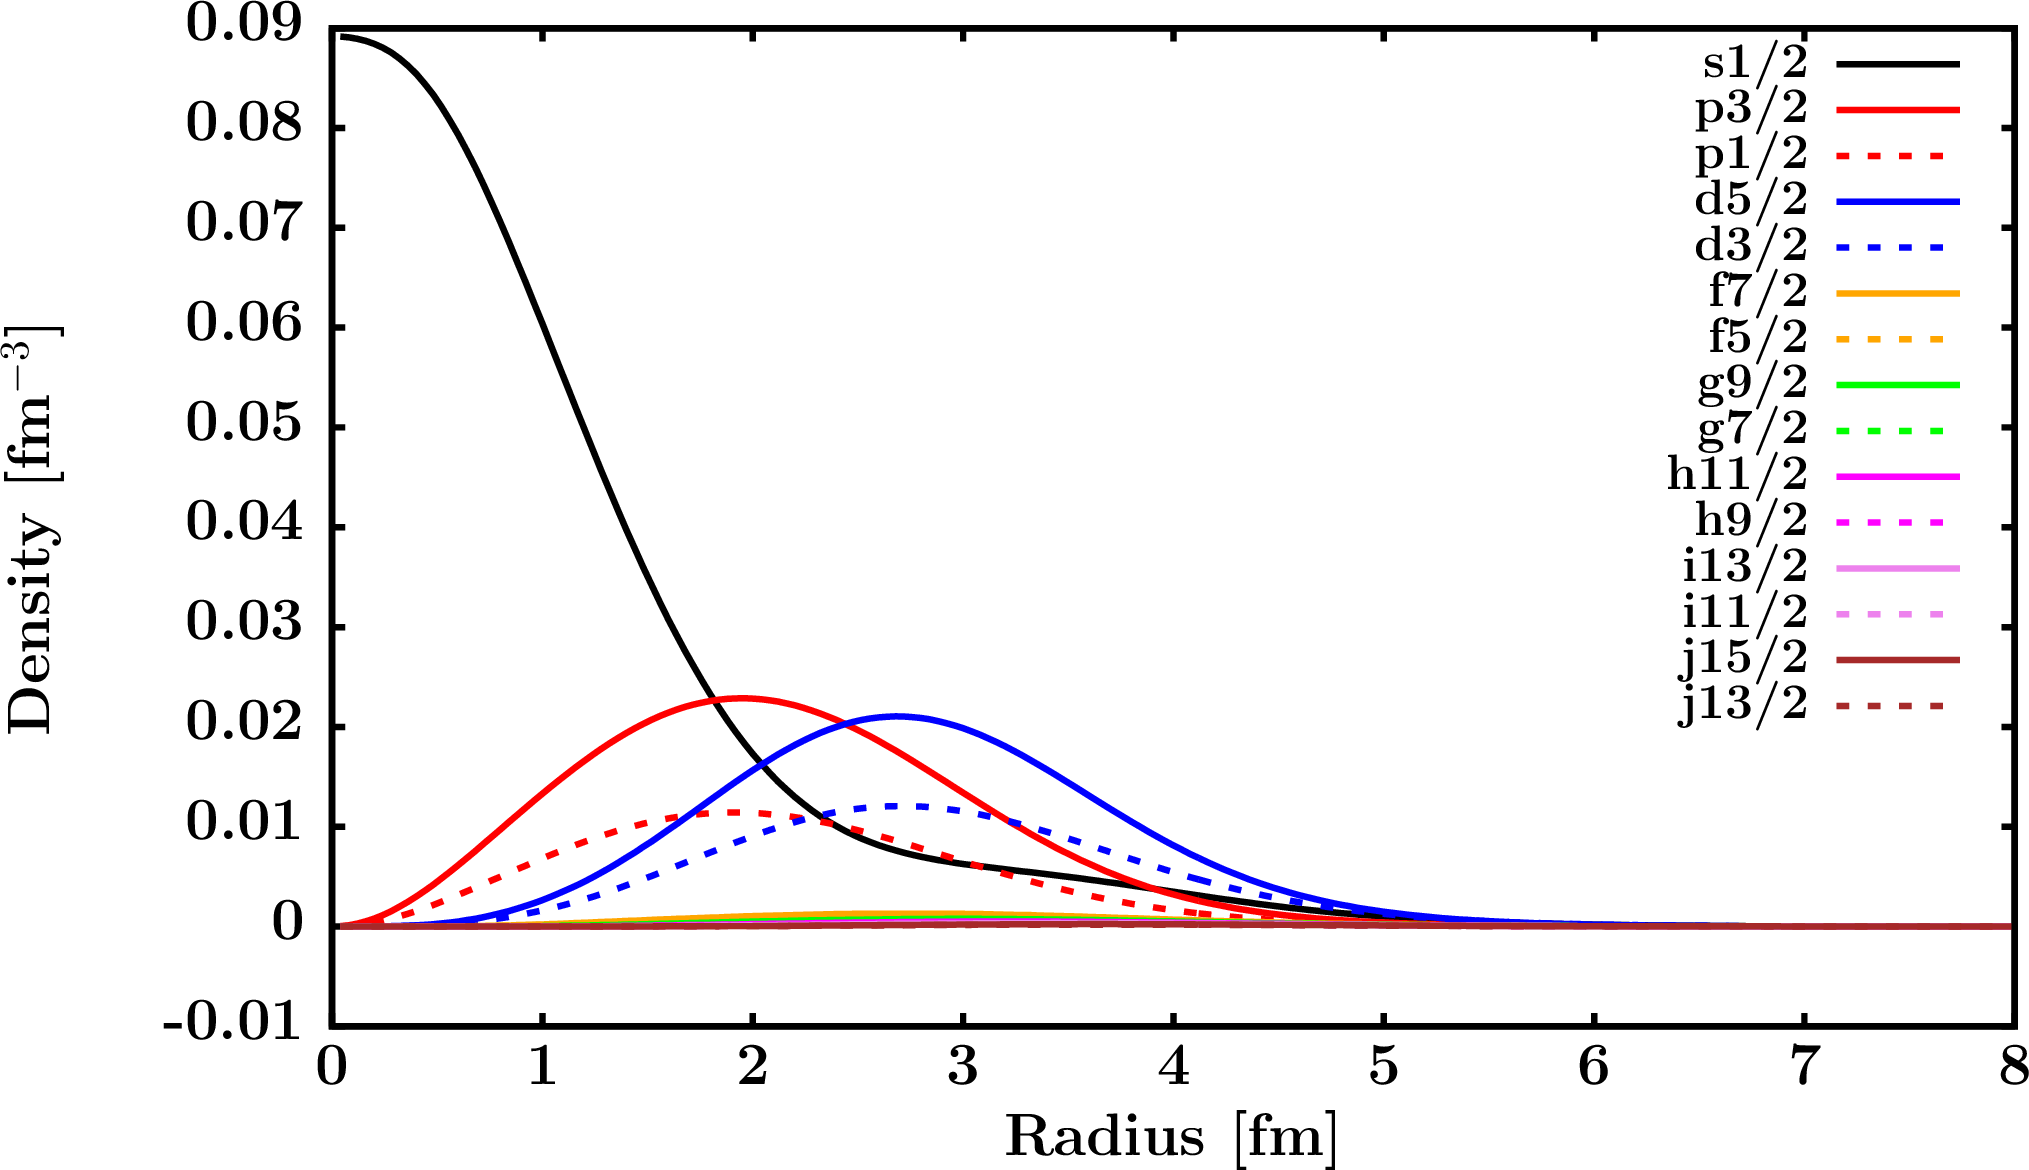
\includegraphics[width=0.75\textwidth]{figures/ca40_protonLJDensityDist.png}
    \caption[Proton single-particle density distributions in \caForty]
    {
        Proton single-particle density distributions in \caForty, as generated
        by our DOM fit. Only the \sOne\ has density at the origin, which
        means that to recover the correct charge density at the origin, the
        occupation of the proton 0\sOne\ and 1\sOne\ in \caForty\ must be
        deplying by 20-30\%. That the bound LJs are significantly
        depleted indicates the importance of
        accounting for short- and long-range correlations when extracting
        structural information.
    }
    \label{s1Depletion}
    \label{Ca40ChargeAndLJDensities}
\end{figure}

\begin{figure}[tb]
    \centering
    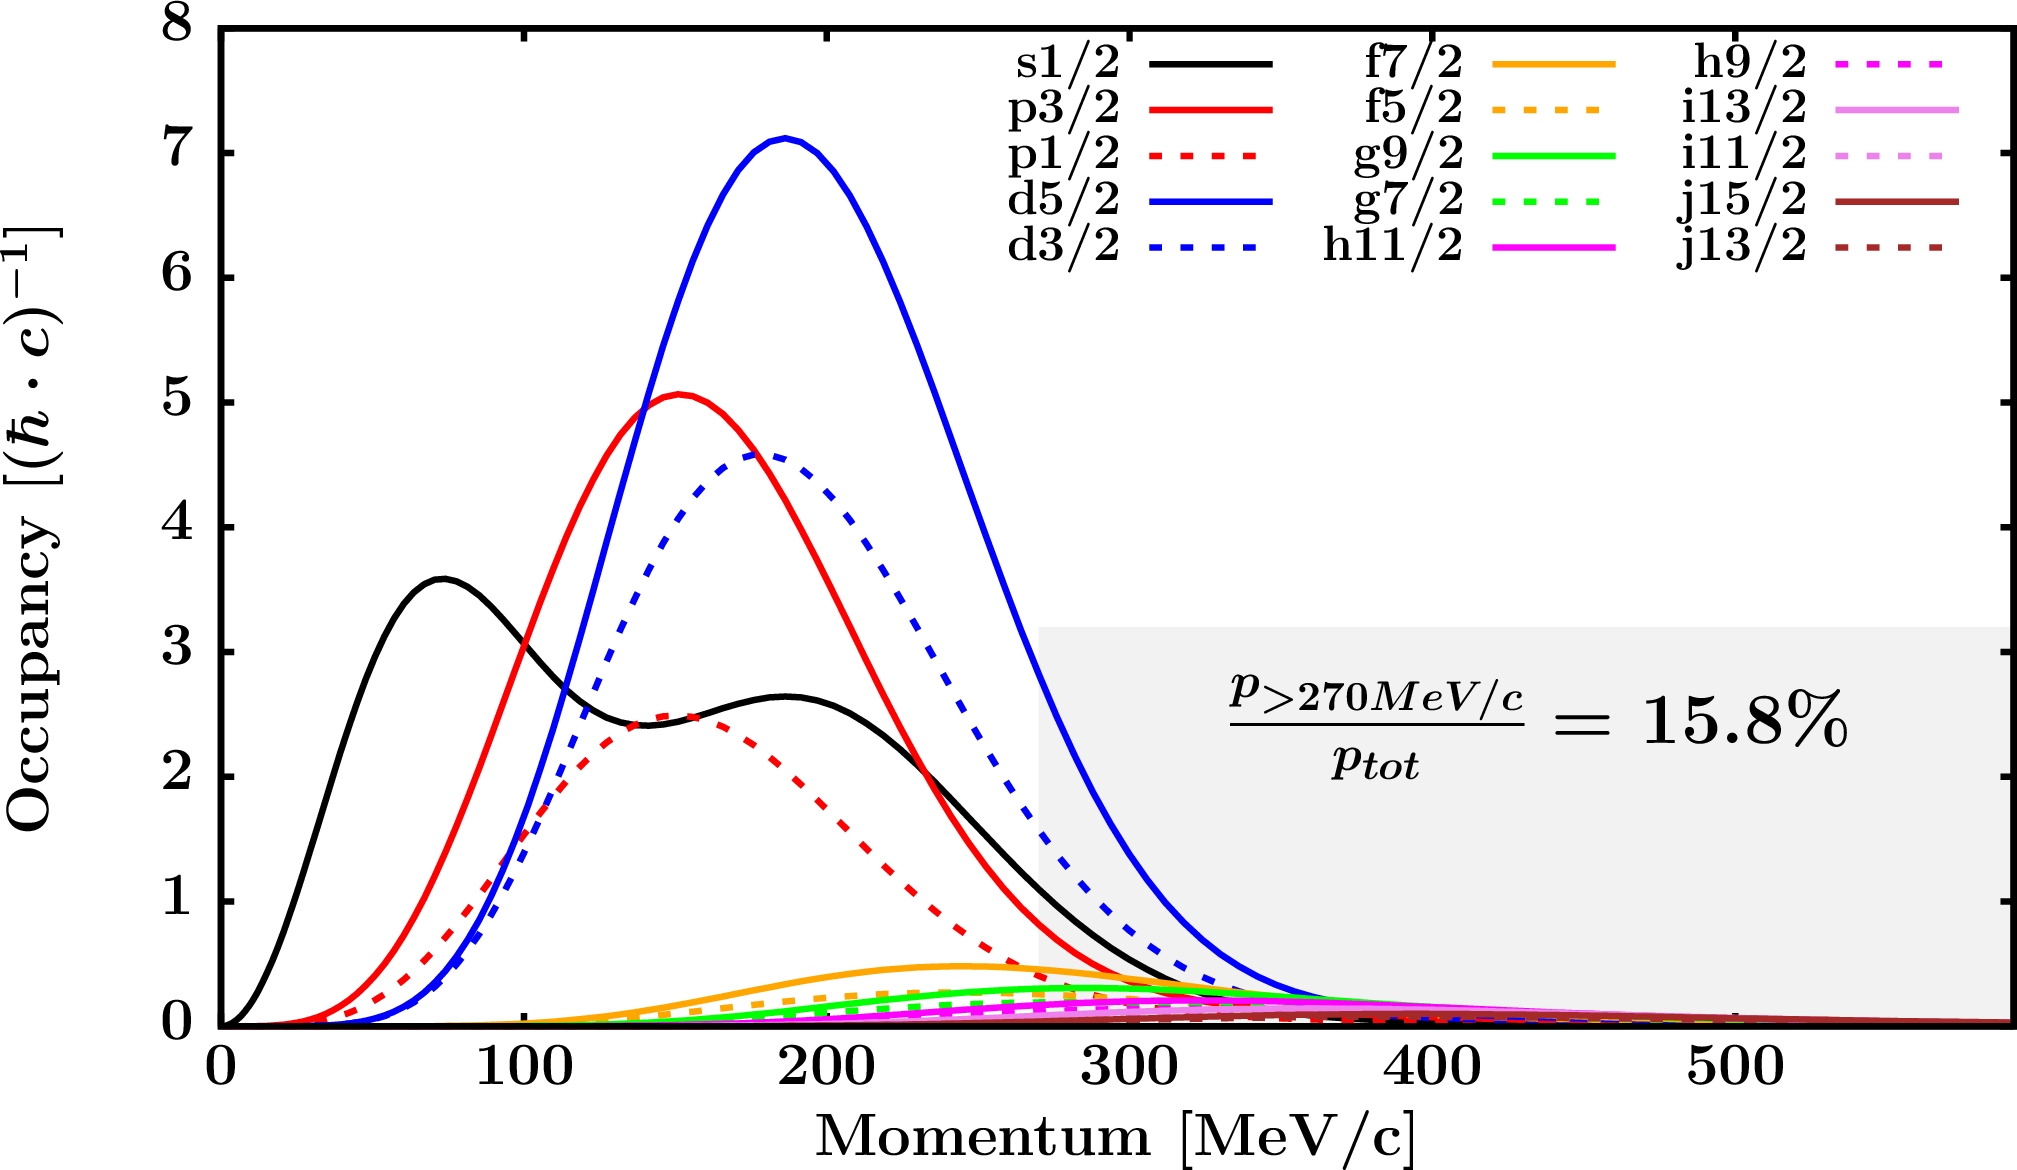
\includegraphics[width=0.75\textwidth]{figures/ca40_protonLJMomentumDistIntegral.png}
    \caption[Proton momentum distribution in \caForty]
    {
        Integrated proton momentum distribution in \caForty, as generated
        by our DOM fit. For the slightly-occupied proton \fSeven, \fFive, and
        \gNine\ and higher shells (which are completely vacant in an
        independent-particle model), a significant fraction of their
        density lies above 270 $\mega\electronvolt/\text{c}$ (indicated by
        the shaded gray region). The fraction of
        proton high-momentum content (i.e., above 270
        $\mega\electronvolt/\text{c}$) is listed.
    }
    \label{Ca40ProtonMomentumDistInt}
    \vspace{16pt}
    \centering
    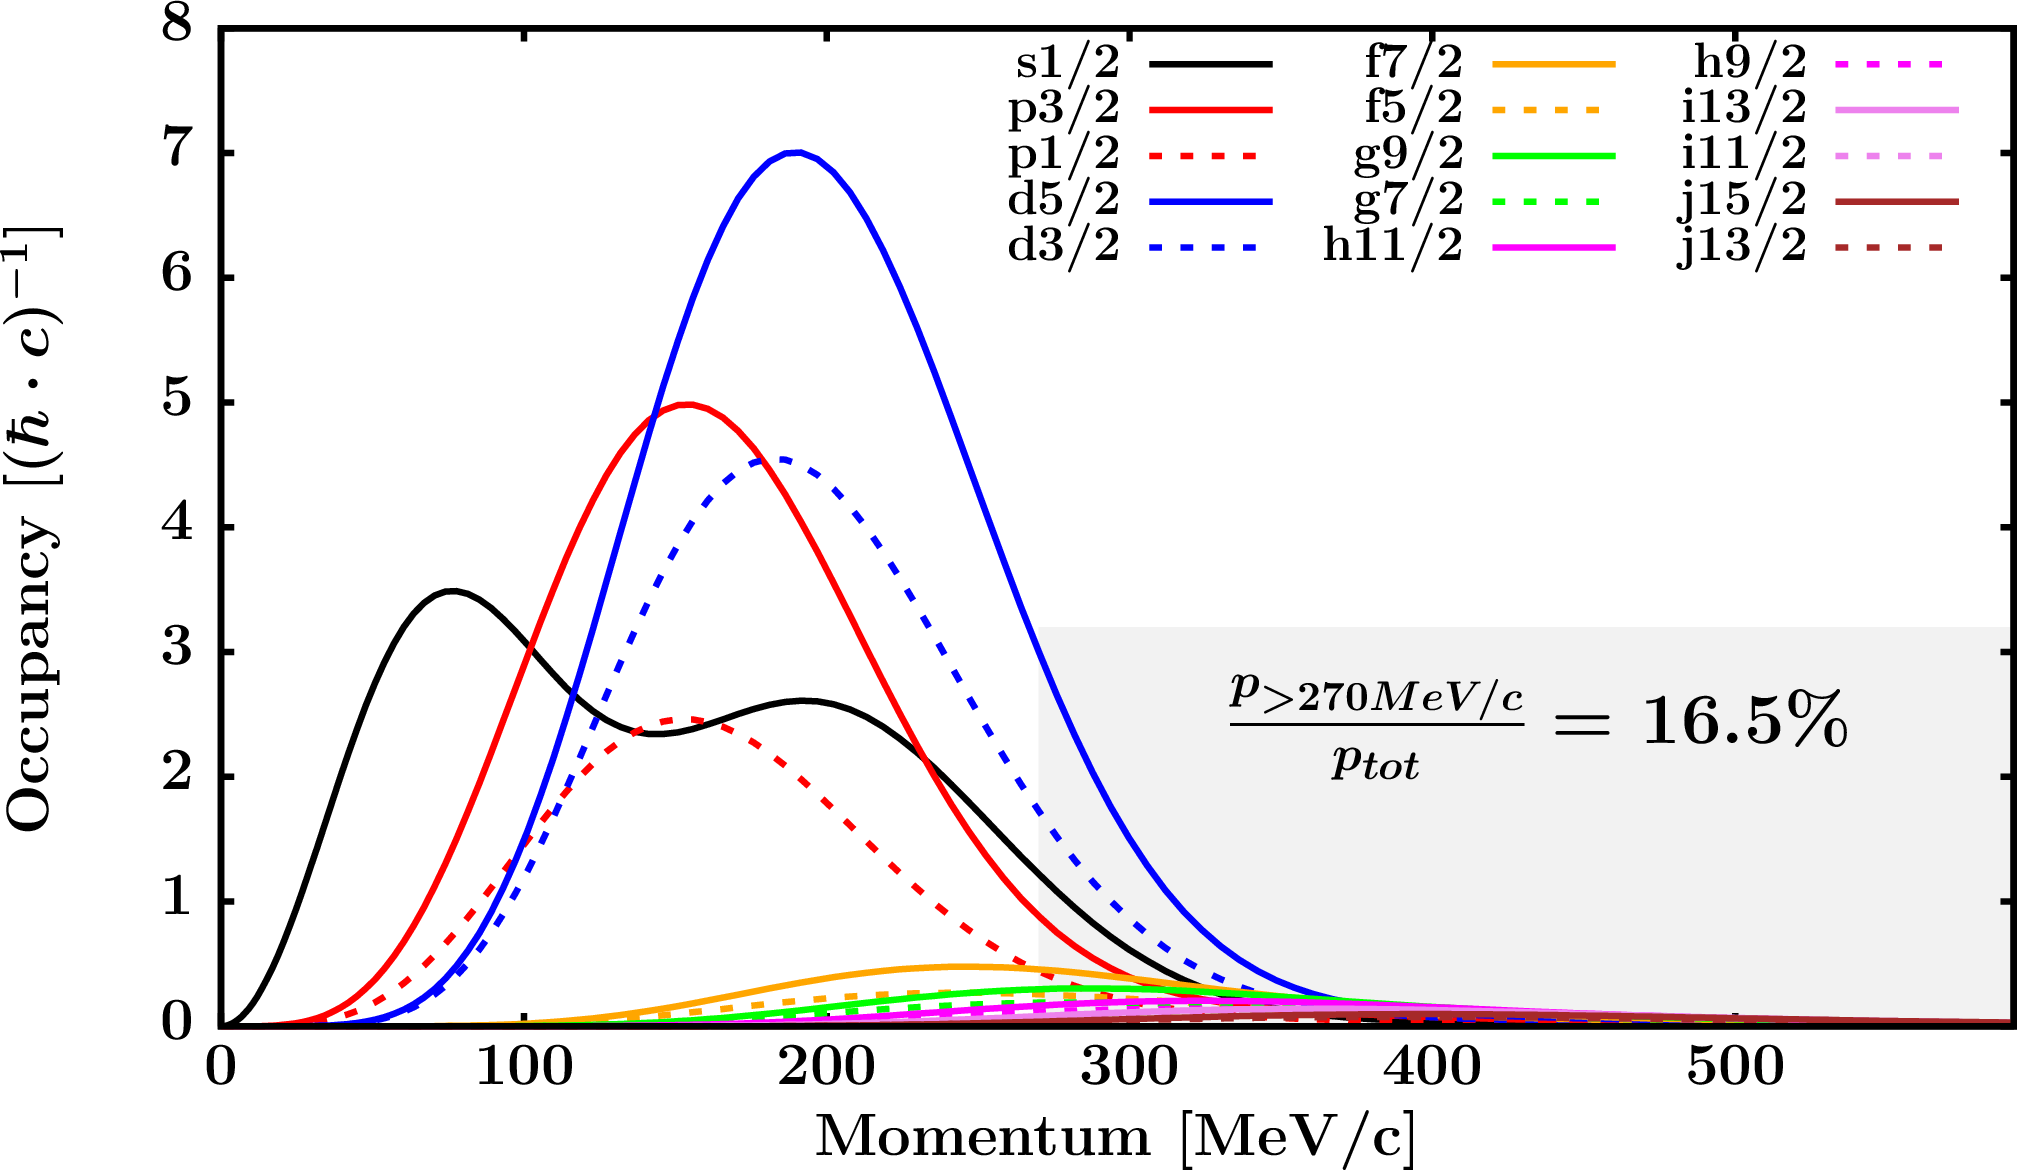
\includegraphics[width=0.75\textwidth]{figures/ca40_neutronLJMomentumDistIntegral.png}
    \caption[Neutron momentum distributions in \caForty]
    {
        Integrated neutron momentum distribution in \caForty, as generated
        by our DOM fit. The slightly-occupied neutron \fSeven, \fFive, and
        \gNine\ shells make a significant contribution to the high-momentum
        content above 270 $\mega\electronvolt/\text{c}$ (indicated by the
        shaded gray region), as is true for the protons in the figure at top
        of the page. The fraction of neutron density with
        momentum above 270 $\mega\electronvolt/\text{c}$ is listed.
    }
    \label{Ca40NeutronMomentumDistInt}
\end{figure}

\begin{figure}[tb]
    \centering
    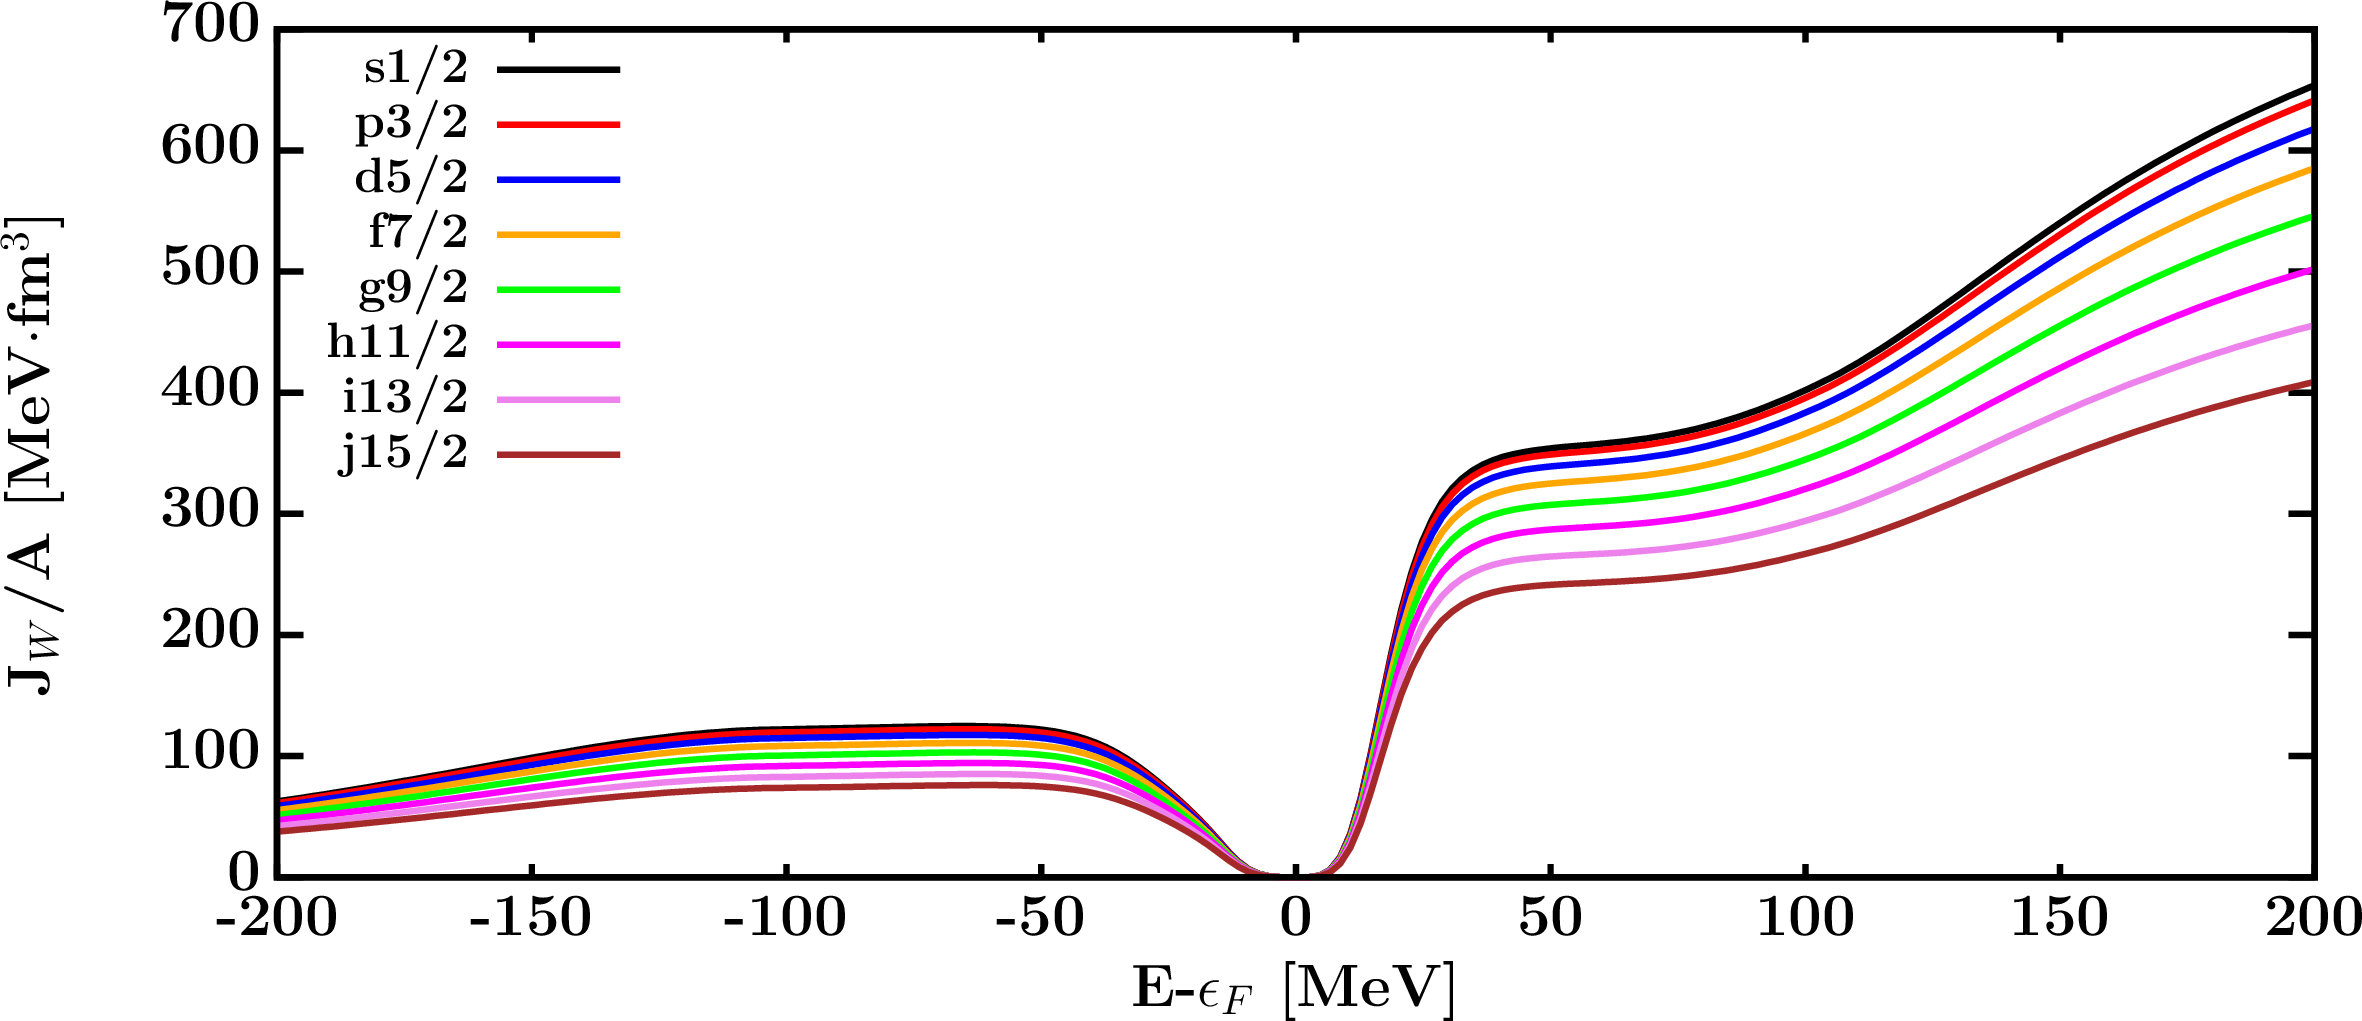
\includegraphics[width=\textwidth]{figures/ca40_protonVolumeIntegrals.png}
    \caption[Volume integral of proton imaginary potential in \caForty]
    {
        Volume integral of proton imaginary potential in \caForty. Above the
        Fermi energy, the surface-associated and volume-associated strength
        are clearly identifiable around 40 MeV and above 100 MeV,
        respectively. Near the Fermi energy, the potential is symmetric.
        Below the Fermi energy, the reduction of phase space reduces the
        magnitude of imaginary strength, but even at very negative energies,
        there is some strength. The small -- but signficant -- occupation at
        very negative energies make an outsized contribution to the total
        binding energy.
    }
    \label{Ca40ProtonVolumeIntegral}
\end{figure}

\begin{figure}[tb]
    \centering
    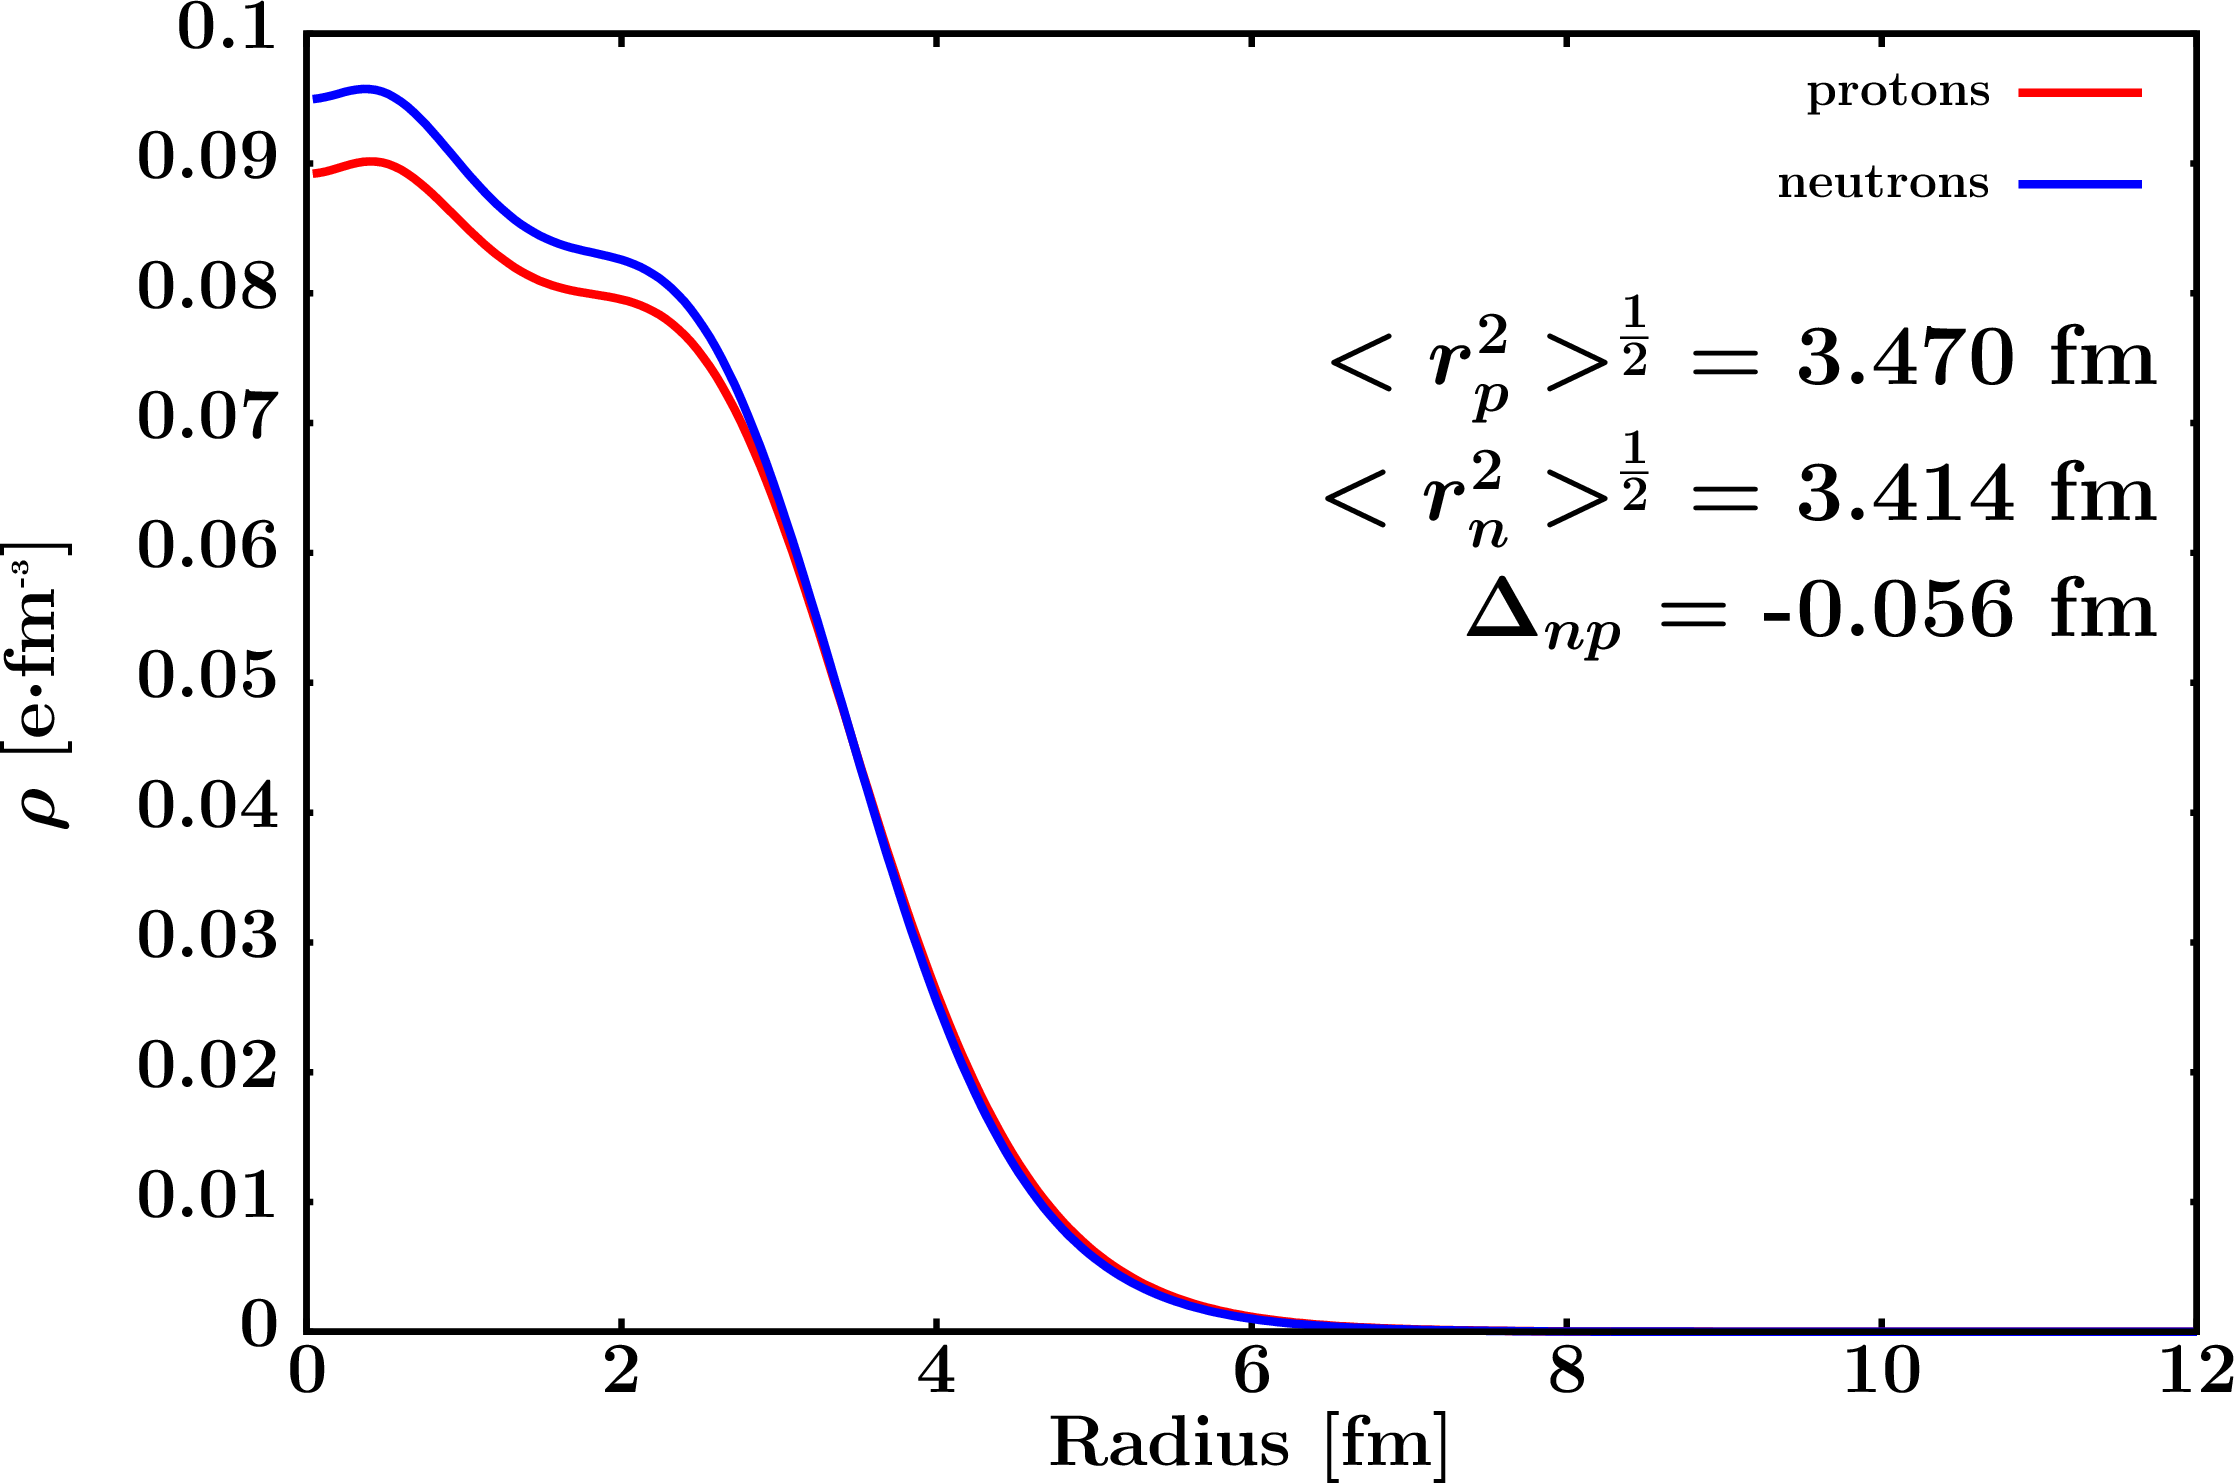
\includegraphics[width=\textwidth]{figures/ca40_matterDensity.png}
    \caption[Proton and neutron matter density distributions in \caForty]
    {
        Proton and neutron point density distributions in \caForty, as
        generated by our DOM fit. The RMS radii of the distributions and their
        difference (the neutron skin) are provided. In a symmetric system like
        \caForty, the neutron skin is expected to be slightly negative as a
        consequence of slight reduction of proton density in the core from
        Coulomb repulsion. The neutron skin we extract is in good agreement with
        the previous DOM fit of \cite{MahzoonPhDThesis}. A comparison to the
        experimental \caForty\ charge density distribution is shown in Section
        \ref{ca40DOMOutput} of Appendix \ref{DOMVisualization}.
    }
    \label{Ca40MatterDistribution}
\end{figure}

\begin{figure}[tb]
    \centering
    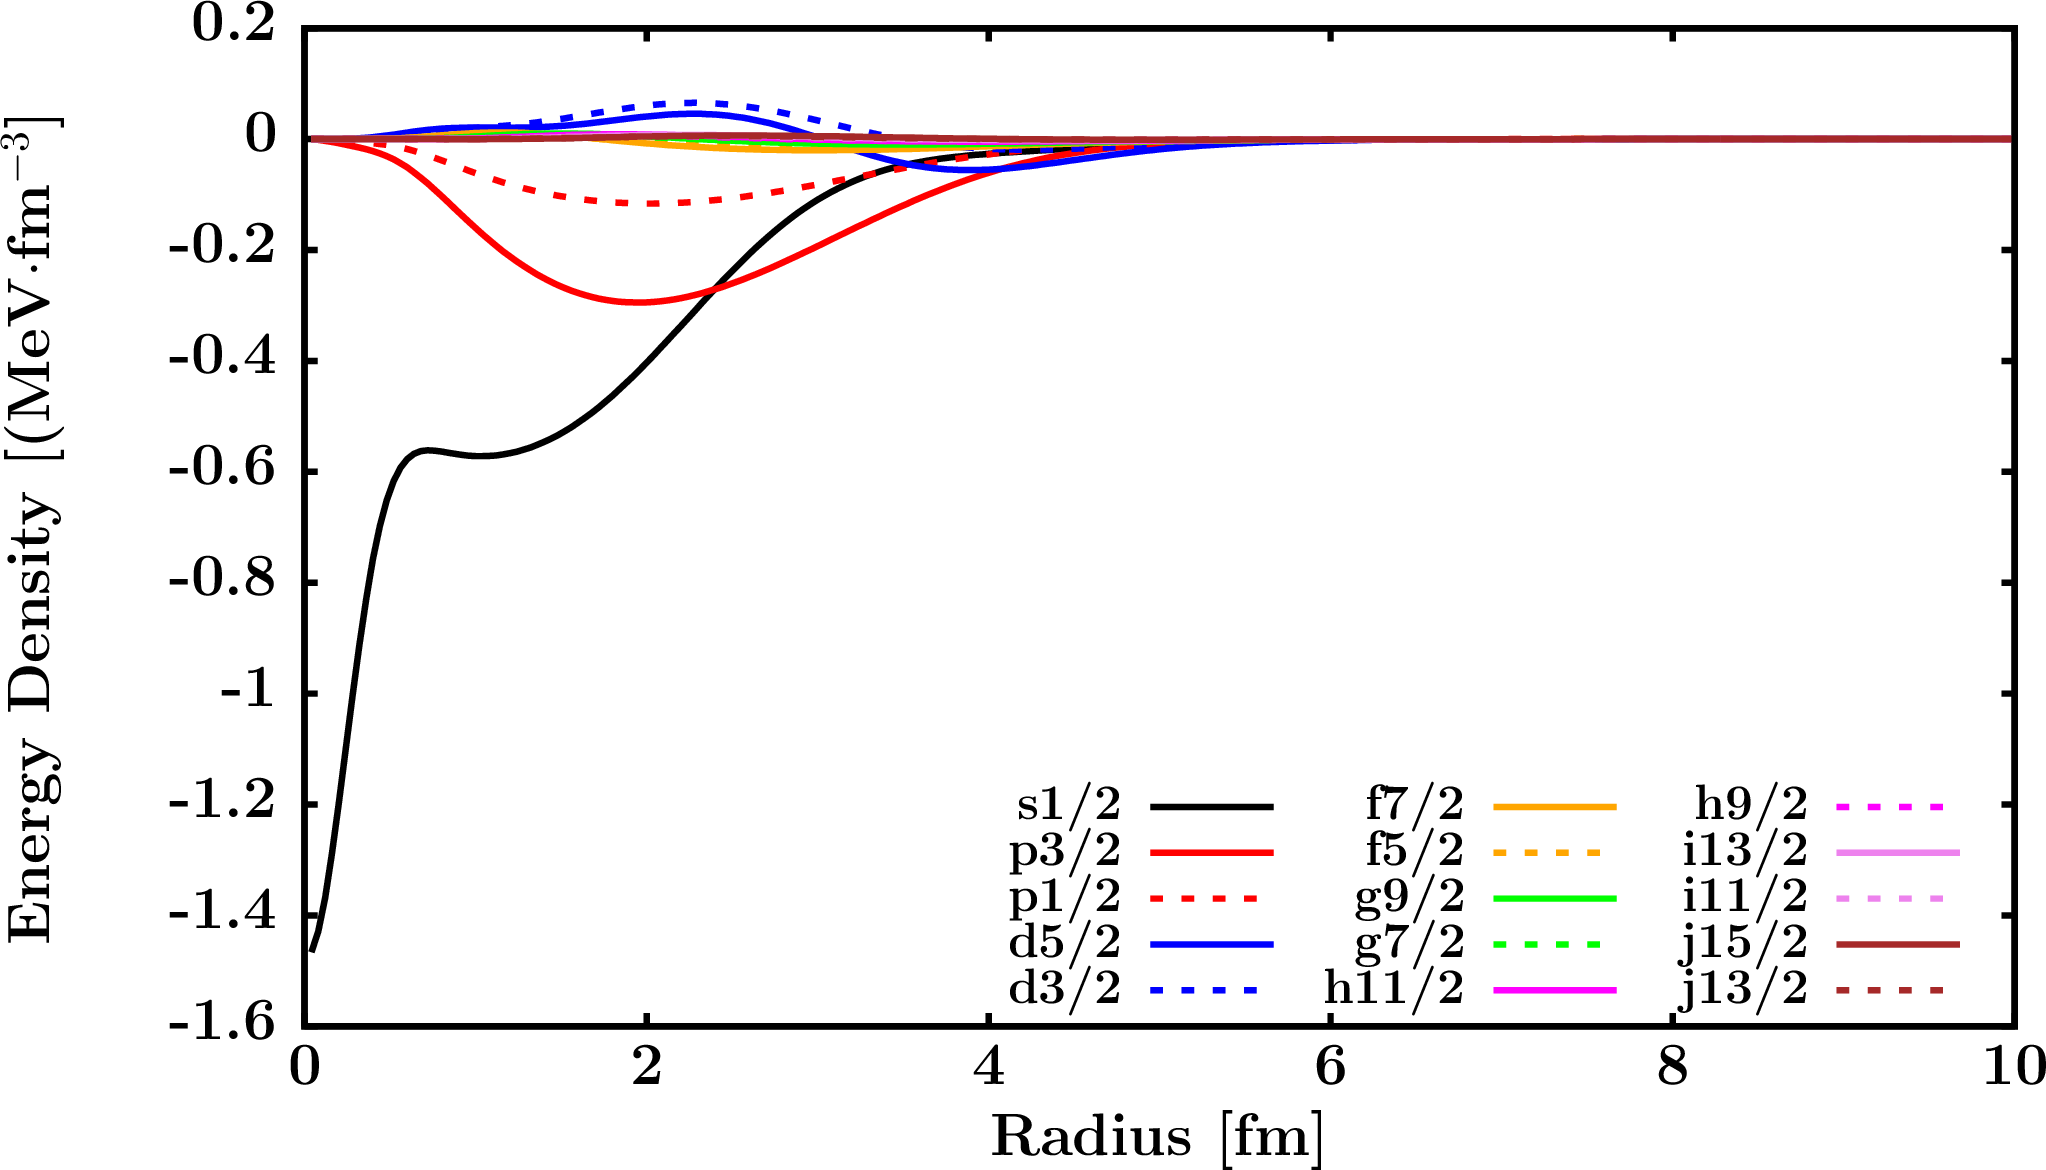
\includegraphics[width=0.75\textwidth]{figures/ca40_EnergyDist.png}
    \caption[Energy density distribution for protons in \caForty]
    {
        Energy density distribution for protons in \caForty, as generated
        by our DOM fit. Valence nucleons (e.g., in the proton 1\sOne\ and
        0\dThree\ subshells in \caForty) contribute only slightly to the binding
        energy.
    }
    \label{Ca40EnergyDist}
    \vspace{16pt}
    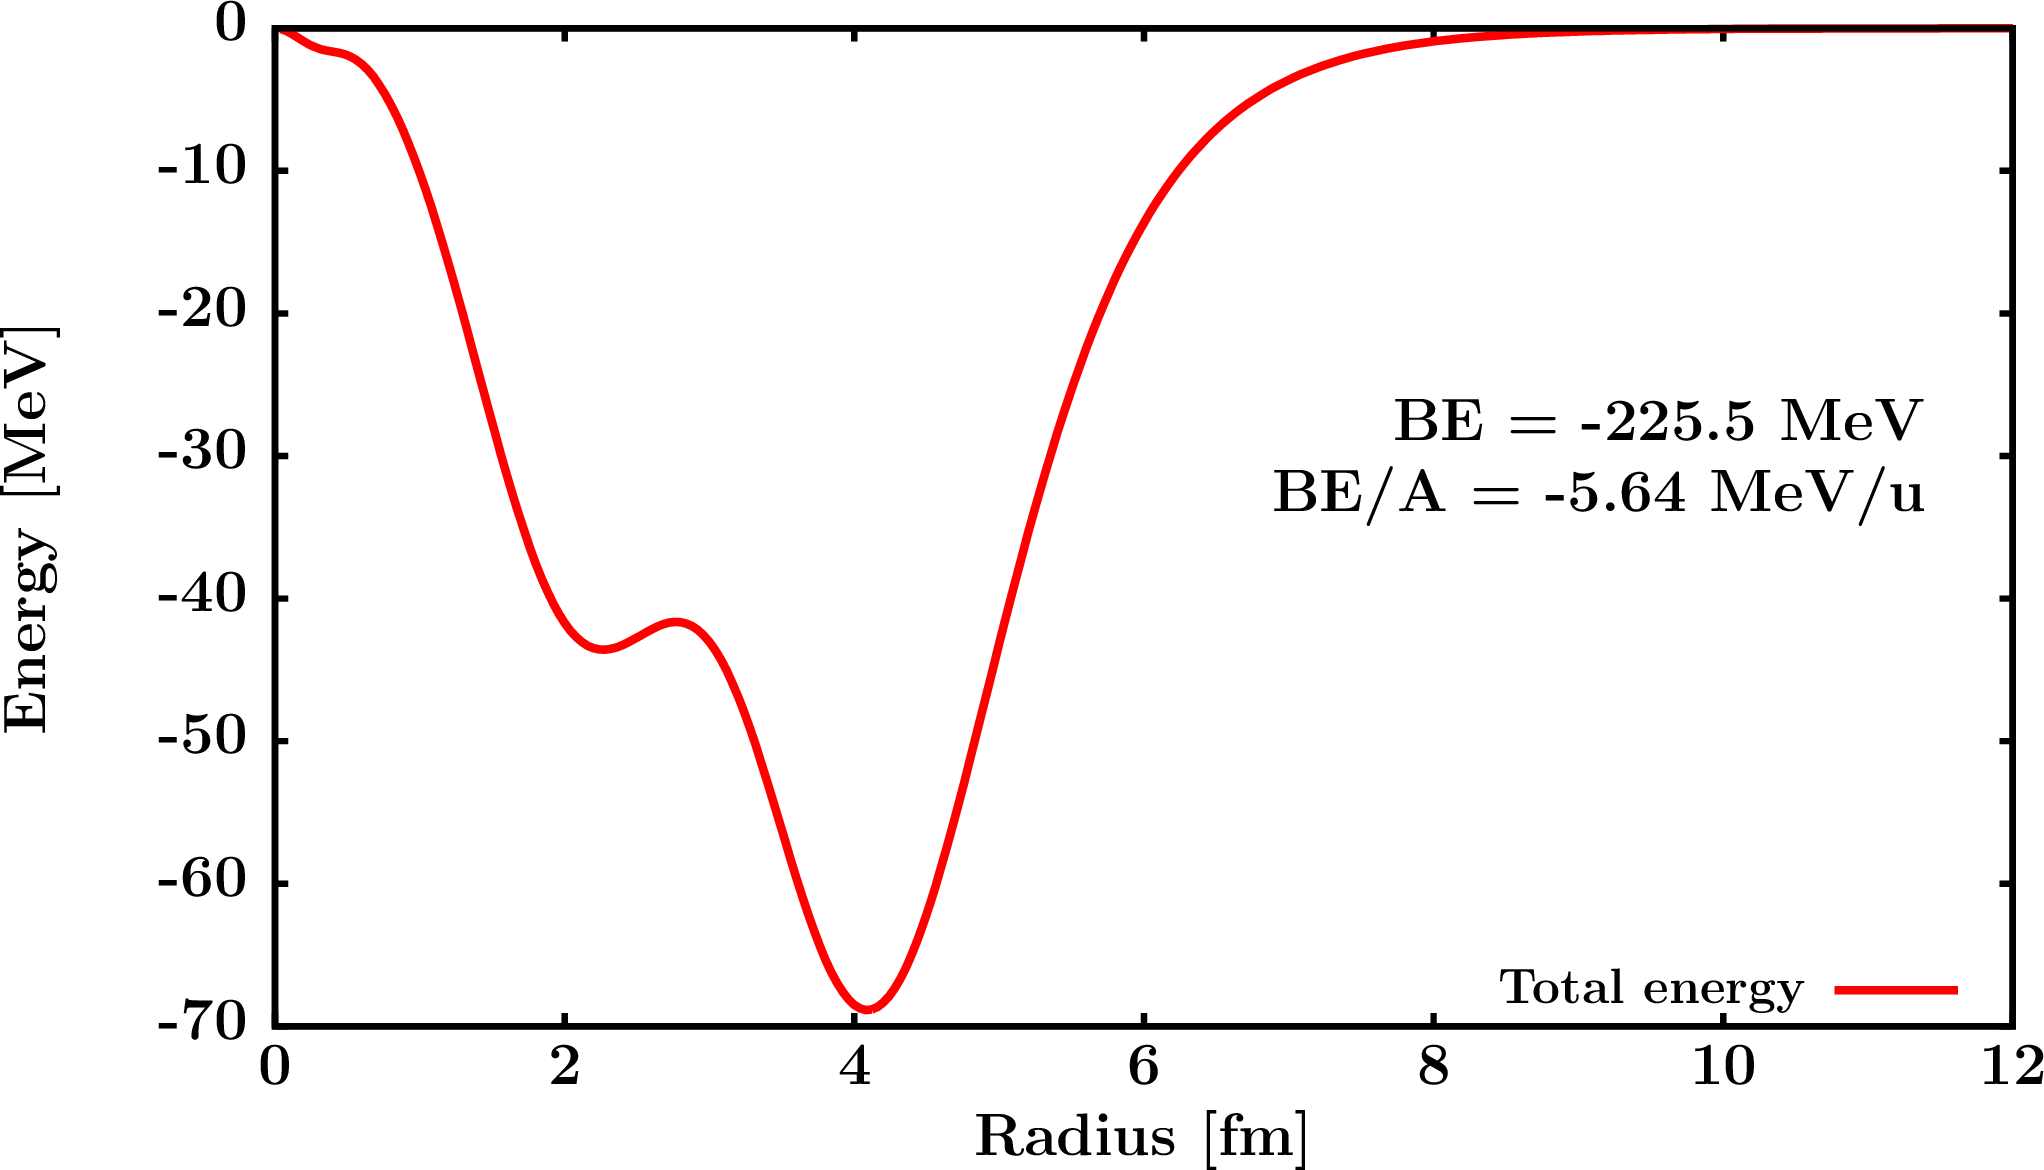
\includegraphics[width=0.75\textwidth]{figures/ca40_EnergyDistIntegral.png}
    \caption[Total energy density integral in \caForty]
    {
        Total energy density integral in \caForty, as generated
        by our DOM fit. The total binding energy and binding energy per
        nucleon are given.
    }
    \label{Ca40EnergyDistIntegral}
\end{figure}

From the spectral functions, the momentum-space distribution for protons and neutrons was
calculated (shown in Figs. \ref{Ca40ProtonMomentumDistInt} and
\ref{Ca40NeutronMomentumDistInt}). 
The amount of ``high-momentum content'' of
these distributions is of great interest, as significant high-momentum content 
indicates deviation from the mean-field picture due to short-range correlations (SRCs). SRCs arise 
even in very light nuclear systems (e.g., \heFour)
and are associated with an altered quark distribution in nucleons 
\cite{Hen2012, Arrington2012, CLAS2019}.
Tensor-force interactions in neutron-proton pairs are thought to be a dominant source of 
SRCs \cite{Subedi2008}. Thus in symmetric nuclei like \cTwelve\ and \caForty, the
high-momentum content is expected to be nearly the same for protons and neutrons, whereas in
asymmetric nuclei like \pbEight, the minority nucleon species is expected to have a larger
high-momentum tail in the momentum distribution. In \cite{Rohe2004}, the \cTwelve\ proton and
neutron momentum distributions showed that $\approx$10\% of the nucleon density
has momentum above roughly 270 $\mega\electronvolt/\text{c}$.
We recover high-momentum fractions of 13.9\% and 14.6\%
for protons and neutrons, respectively.

The total binding energy for \caForty\ is readily calculated using Eq.
\ref{TotalEnergyEquation}. Its radial dependence is shown in Fig.
\ref{Ca40EnergyDistIntegral} and the
contributions to the binding energy from each single-particle LJ are shown in
\ref{Ca40EnergyDist}. Per our fit, even though the 0\sOne\ nucleons are
only about 9\% of the total nucleons in \caForty, they provide a significant
share of the binding
energy (35\%). As the spectral
functions (Fig. \ref{Ca40SpectralFunctions}) reveal, 0\sOne\ nucleons spend a small but significant portion of their time 
at very negative energies ($<$-100 \mega\electronvolt), pulling the weighted average binding energy 
closer to 8.5 \mega\electronvolt/A, the experimentally-known binding energy
for \caForty. Even in our fits that posses a large negative-energy tail, we
still underpredict the binding by roughly 2 \mega\electronvolt/A. It appears
that a better description of nucleon-nucleon correlations at extreme
negative energies is required to locate the remaining binding energy.

Lastly, from the proton and neutron point distributions generated by our fit, we calculate a
\caForty\ neutron skin for of -0.056 \femto\meter\ (see Fig. \ref{Ca40MatterDistribution}). 
This is in good agreement with the skin calculated in previous DOM treatments
\cite{MahzoonPhDThesis} and with the expectation that the neutron skin should be slightly negative in
symmetric nuclei, a consequence of Coulomb repulsion nudging proton density toward the surface.

\subsection{Results for \caEight}
The recent non-local DOM treatment of Mahzoon et al. \cite{Mahzoon2017} was able
to reproduce a wide variety of
experimental data on \caEight\ and recovered a \caEight\ neutron
skin of 0.249 $\pm$ 0.023 \femto\meter.
This neutron skin value is significantly higher than the 0.132 \femto\meter\ calculated by
the \textit{ab initio} treatment of \cite{Hagen2016}. Mahzoon et al. found that when the 
smaller \textit{ab initio} was forcibly applied to their fit, it disturbed the fit's
reproduction of experimental \caEight\ neutron \tot\ data, implying that the neutron \tot\ might
be sensitive to the neutron skin thickness. In this work, our fit on \caEight\ uses essentially the 
same experimental data used by Mahzoon et al. but less than half as many potential parameters.

There are fewer available elastic nucleon scattering data sets for \caEight\ compared to \caForty,
so it was somewhat more difficult to nail down the real terms of the potential. Still, with both
proton elastic scattering data sets a complete neutron total cross section data set in hand, we did
not have too much trouble converging on a reasonable asymmetry-dependence for the depth of the real
central potential $V_{asym}$. This term sets the relative depth of the central potential for protons 
and neutrons and thus is moderately important for the size of the neutron skin. A more serious
problem was the lack of proton \rxn\ data above 48 MeV, as it meant that the magnitude parameter
of the imaginary volume asymmetry $A_{vol, asym}^{\pm}$ was very difficult to constrain. In our
final optimization, we have a rather low value of $W_{vol}^{+}$ for \caEight\ compared to that of
\caForty\ (compare Fig. \ref{Ca40ProtonVolumeIntegral} with Fig.
\ref{Ca48ProtonVolumeIntegral}).

\begin{figure}[tb]
    \centering
    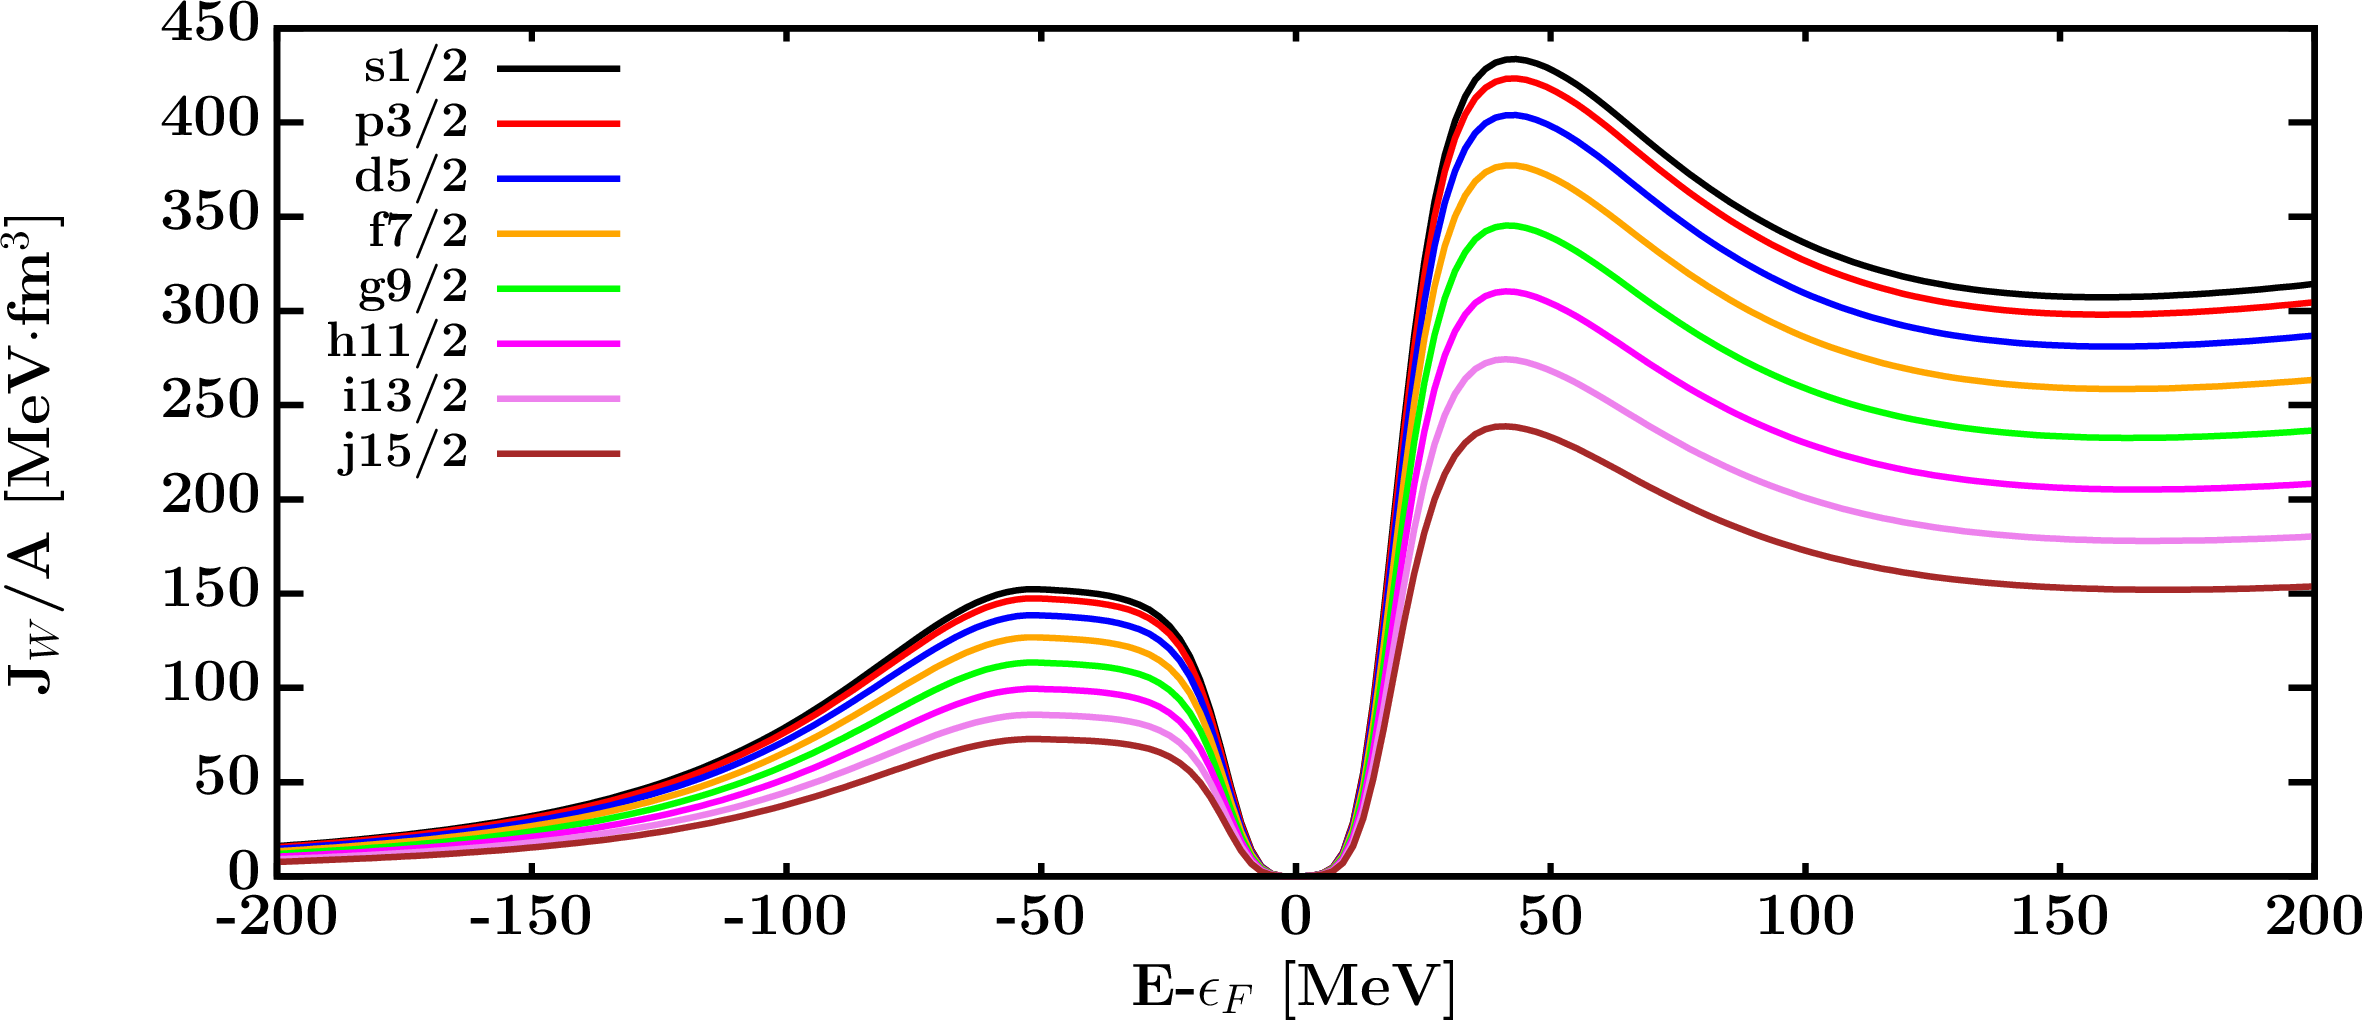
\includegraphics[width=\textwidth]{figures/ca48_protonVolumeIntegrals.png}
    \caption[Volume integral of proton imaginary potential in \caEight]
    {
        Volume integral of proton imaginary potential in \caEight.
        Compared to \caForty, the magnitude and slope
        above 100 \mega\electronvolt\ is significantly lower, likely
        because there were no proton \rxn\ data
        available for \caEight\ above 48 \mega\electronvolt\ to constrain this
        regime.
    }
    \label{Ca48ProtonVolumeIntegral}
\end{figure}

\begin{figure}[tb]
    \centering
    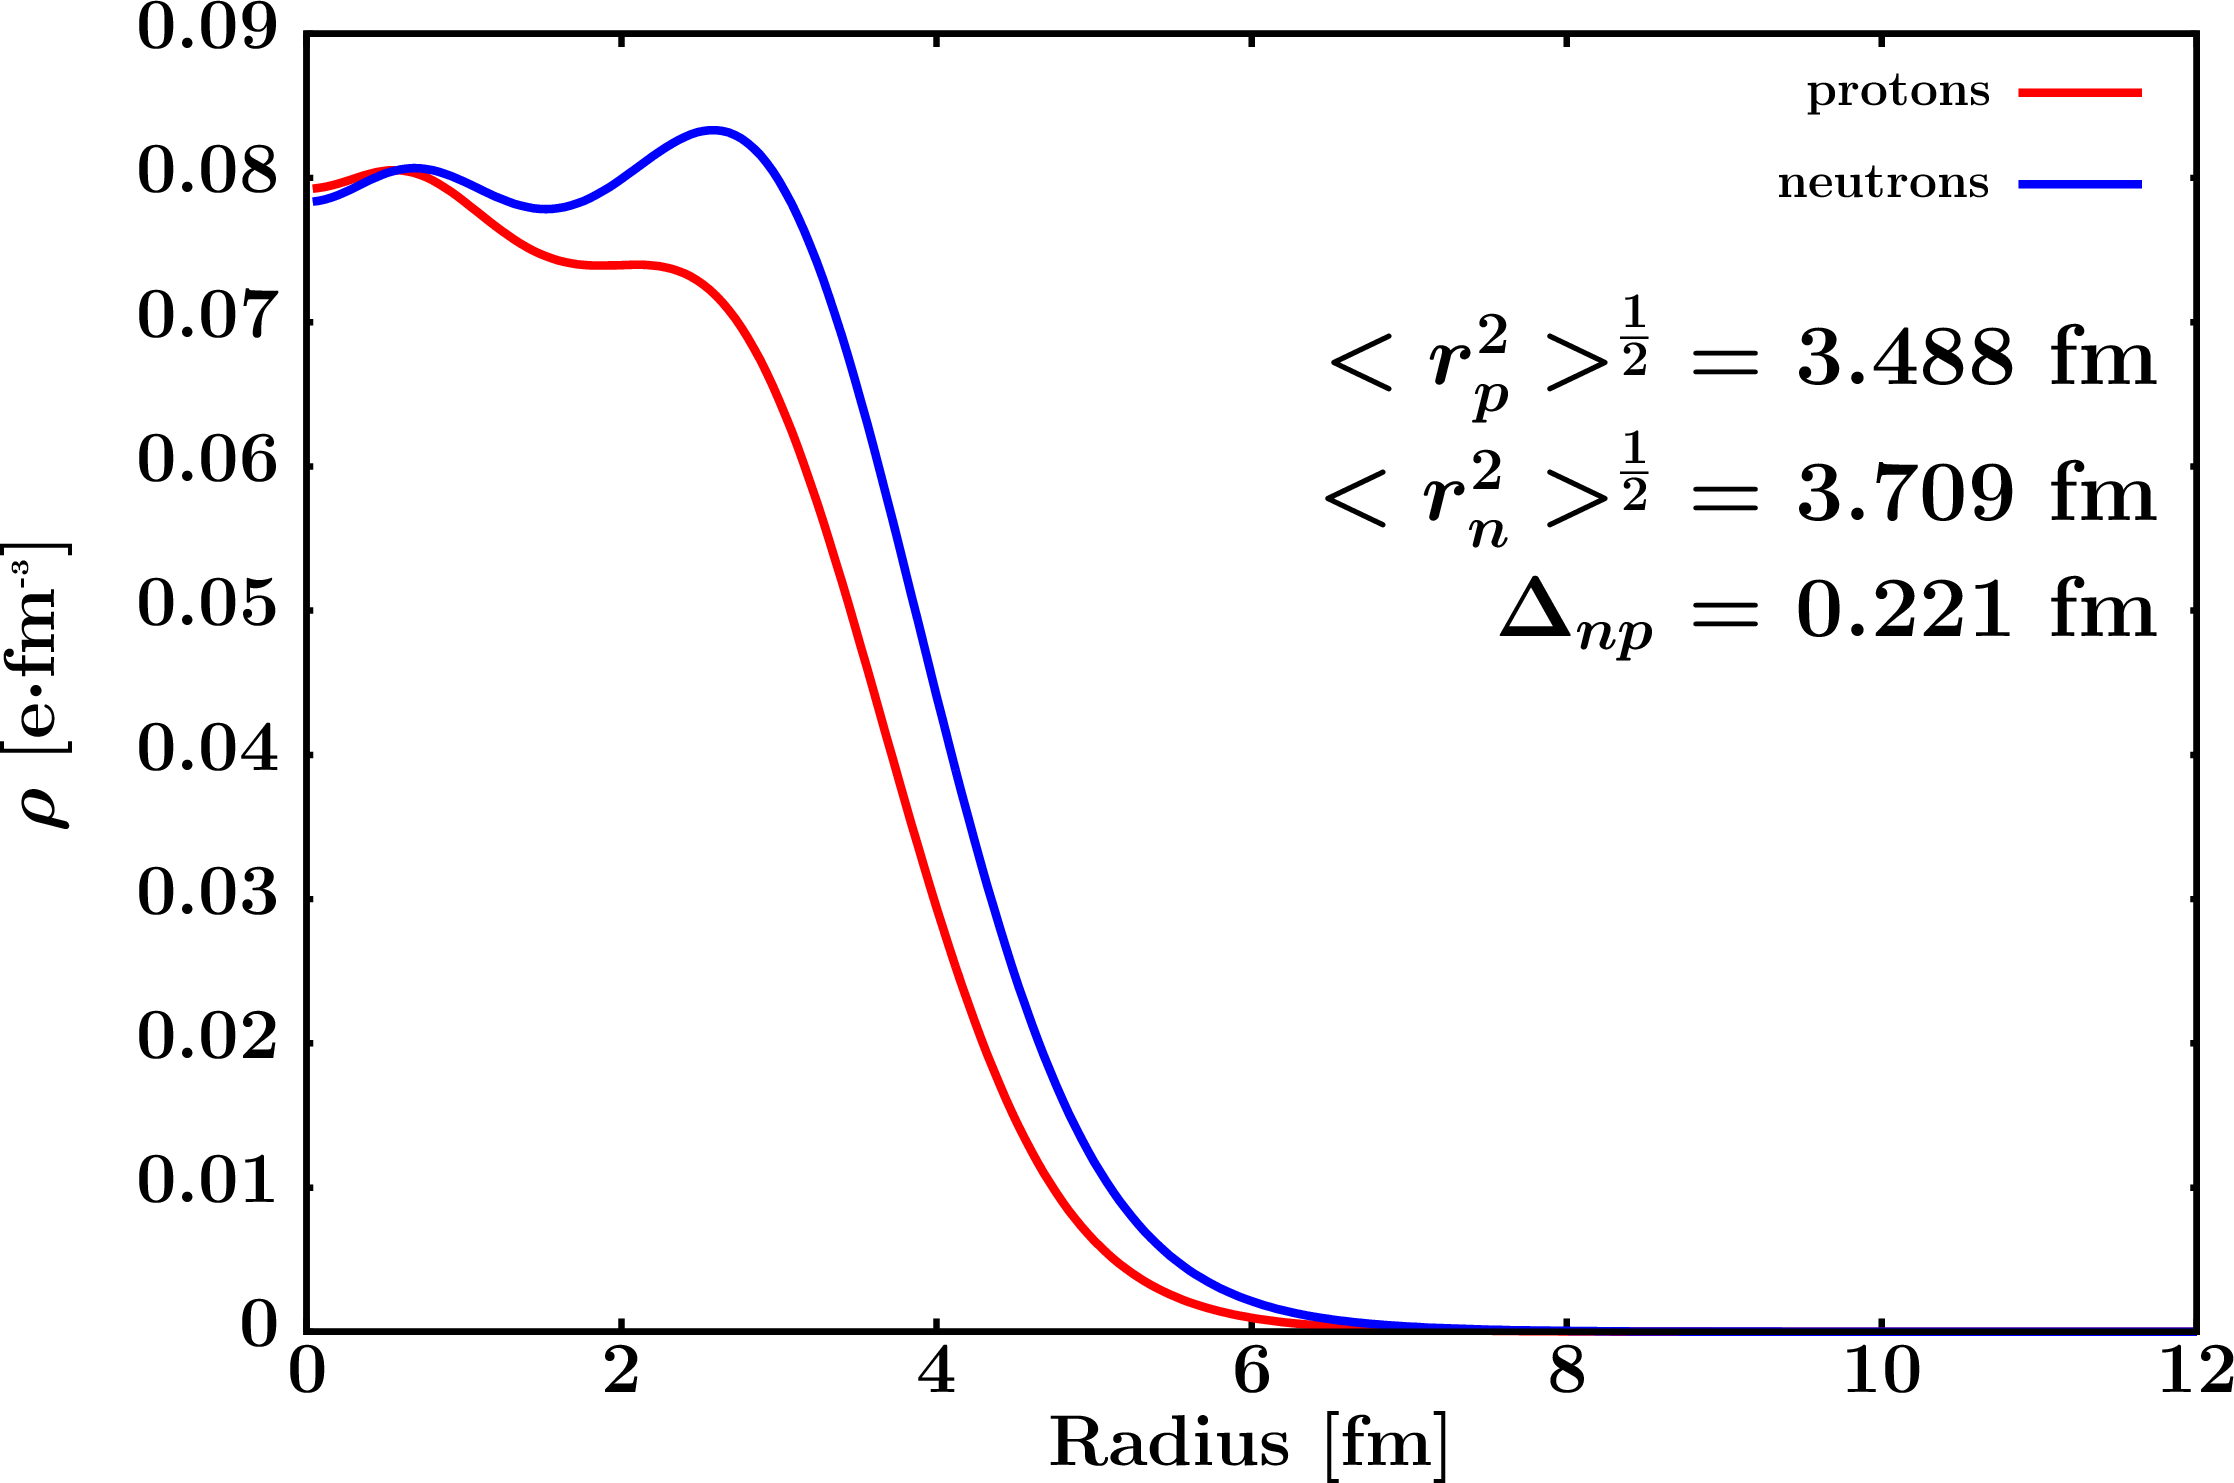
\includegraphics[width=\textwidth]{figures/ca48_matterDensity.png}
    \caption[Proton and neutron matter density distributions in \caEight]
    {
        Proton and neutron point density distributions in \caEight, as
        generated by our DOM fit. The RMS radii of the distributions and their
        difference (the neutron skin) are provided. The neutron
        skin we extract is significantly smaller
        that of the previous DOM fit of \cite{MahzoonPhDThesis} and is only
        slightly larger than the skin extracted from the \textit{ab initio}
        treatment of \cite{Hagen2016}. A comparison with the
        experimental \caEight\ charge density distribution is shown in Section
        \ref{ca48DOMOutput} of Appendix \ref{DOMVisualization}.
    }
    \label{Ca48MatterDist}
\end{figure}

Figure \ref{Ca48MatterDist} shows the matter density distribution of \caEight\ per
our fit. Compared to \caForty, the difference in proton and neutron distributions is more apparent,
as the valence $\nu$0\fSeven\ shell goes
from mostly empty in \caForty\ (0.42 neutrons, per our fit) to 
mostly full in \caEight\ (6.84 neutrons, per our fit).
We extract a neutron skin of 0.150 \femto\meter,
significantly lower than the 0.249$\pm$ 0.023 \femto\meter\ of the previous DOM treatment
and only slightly larger than the \textit{ab initio} result. Without a covariance analysis of the DOM
parameters, it cannot be clear which DOM result is more reliable.
If most of the additional parameters of
\cite{MahzoonPhDThesis} are well-constrained, then our present treatment with fewer parameters is 
likely deficient, as we would have discarded relevant physics. If the previous treatment
was underconstrained, the previous DOM result may be a consequence of overfitting. We
await the results of the CREX measurement to provide a model-independent indication
of the \caEight\ neutron skin size.

\section{Results for \oSixEight}
The lightest system analyzed in the DOM framework, \oSix\ is a valuable benchmark
for $\chi$-EFT, shell model, and ab initio approaches. A wealth of scattering and
bound-state information have been collected on \oSix, making it a good test case for the validity
of the DOM in light systems and helping to validate the choices of DOM potential forms.

Of the nuclides we chose for a DOM treatment, \oEight\ was one of most challenging due to the 
paucity of
available experimental data, the lightness of the system, and the neutron open shell.
To constrain the negative-energy domain
of the potential, the only unambiguous experimental data were the neutron and proton separation
energies and the overall binding energy, adding to the uncertainty in the
\oEight\ negative energy parameter values.

\subsection{Results for \oSix}
The large corpus of experimental data used to constrain the \oSix\
potential includes proton \el\ and analyzing powers up to 200 MeV, neutron \el\ and analyzing powers
up to 100 MeV, proton \rxn\ cross section up to 65 MeV, and qualitative knowledge about the shape of
the spectral functions of the bound $\pi$ \sOne, \pThree, and \pOne\ subshells from (e,e'p)
measurements. Reasonable agreement with all 
experimental data was achieved, excepting the highest-energy ($>$ 150 \mega\electronvolt)
proton differential elastic cross sections and analyzing powers, especially at backward angles.

For a system as light as \oSix, the density of states at low energies (i.e., below the neutron
separation energy) is sufficiently low that a smoothly-varying potential will be a poor
approximation of the resonance structure that dictates the strength of inelastic scattering. This
deficiency is particularly acute in the doubly-closed-shell nuclei, where the level spacing is
larger near the Fermi energy. We expect this to be a contributing factor to the slight
overestimation of the RMS charge radius (see Fig. \ref{o16ChargeDensity}).

\begin{figure}[tb]
    \centering
    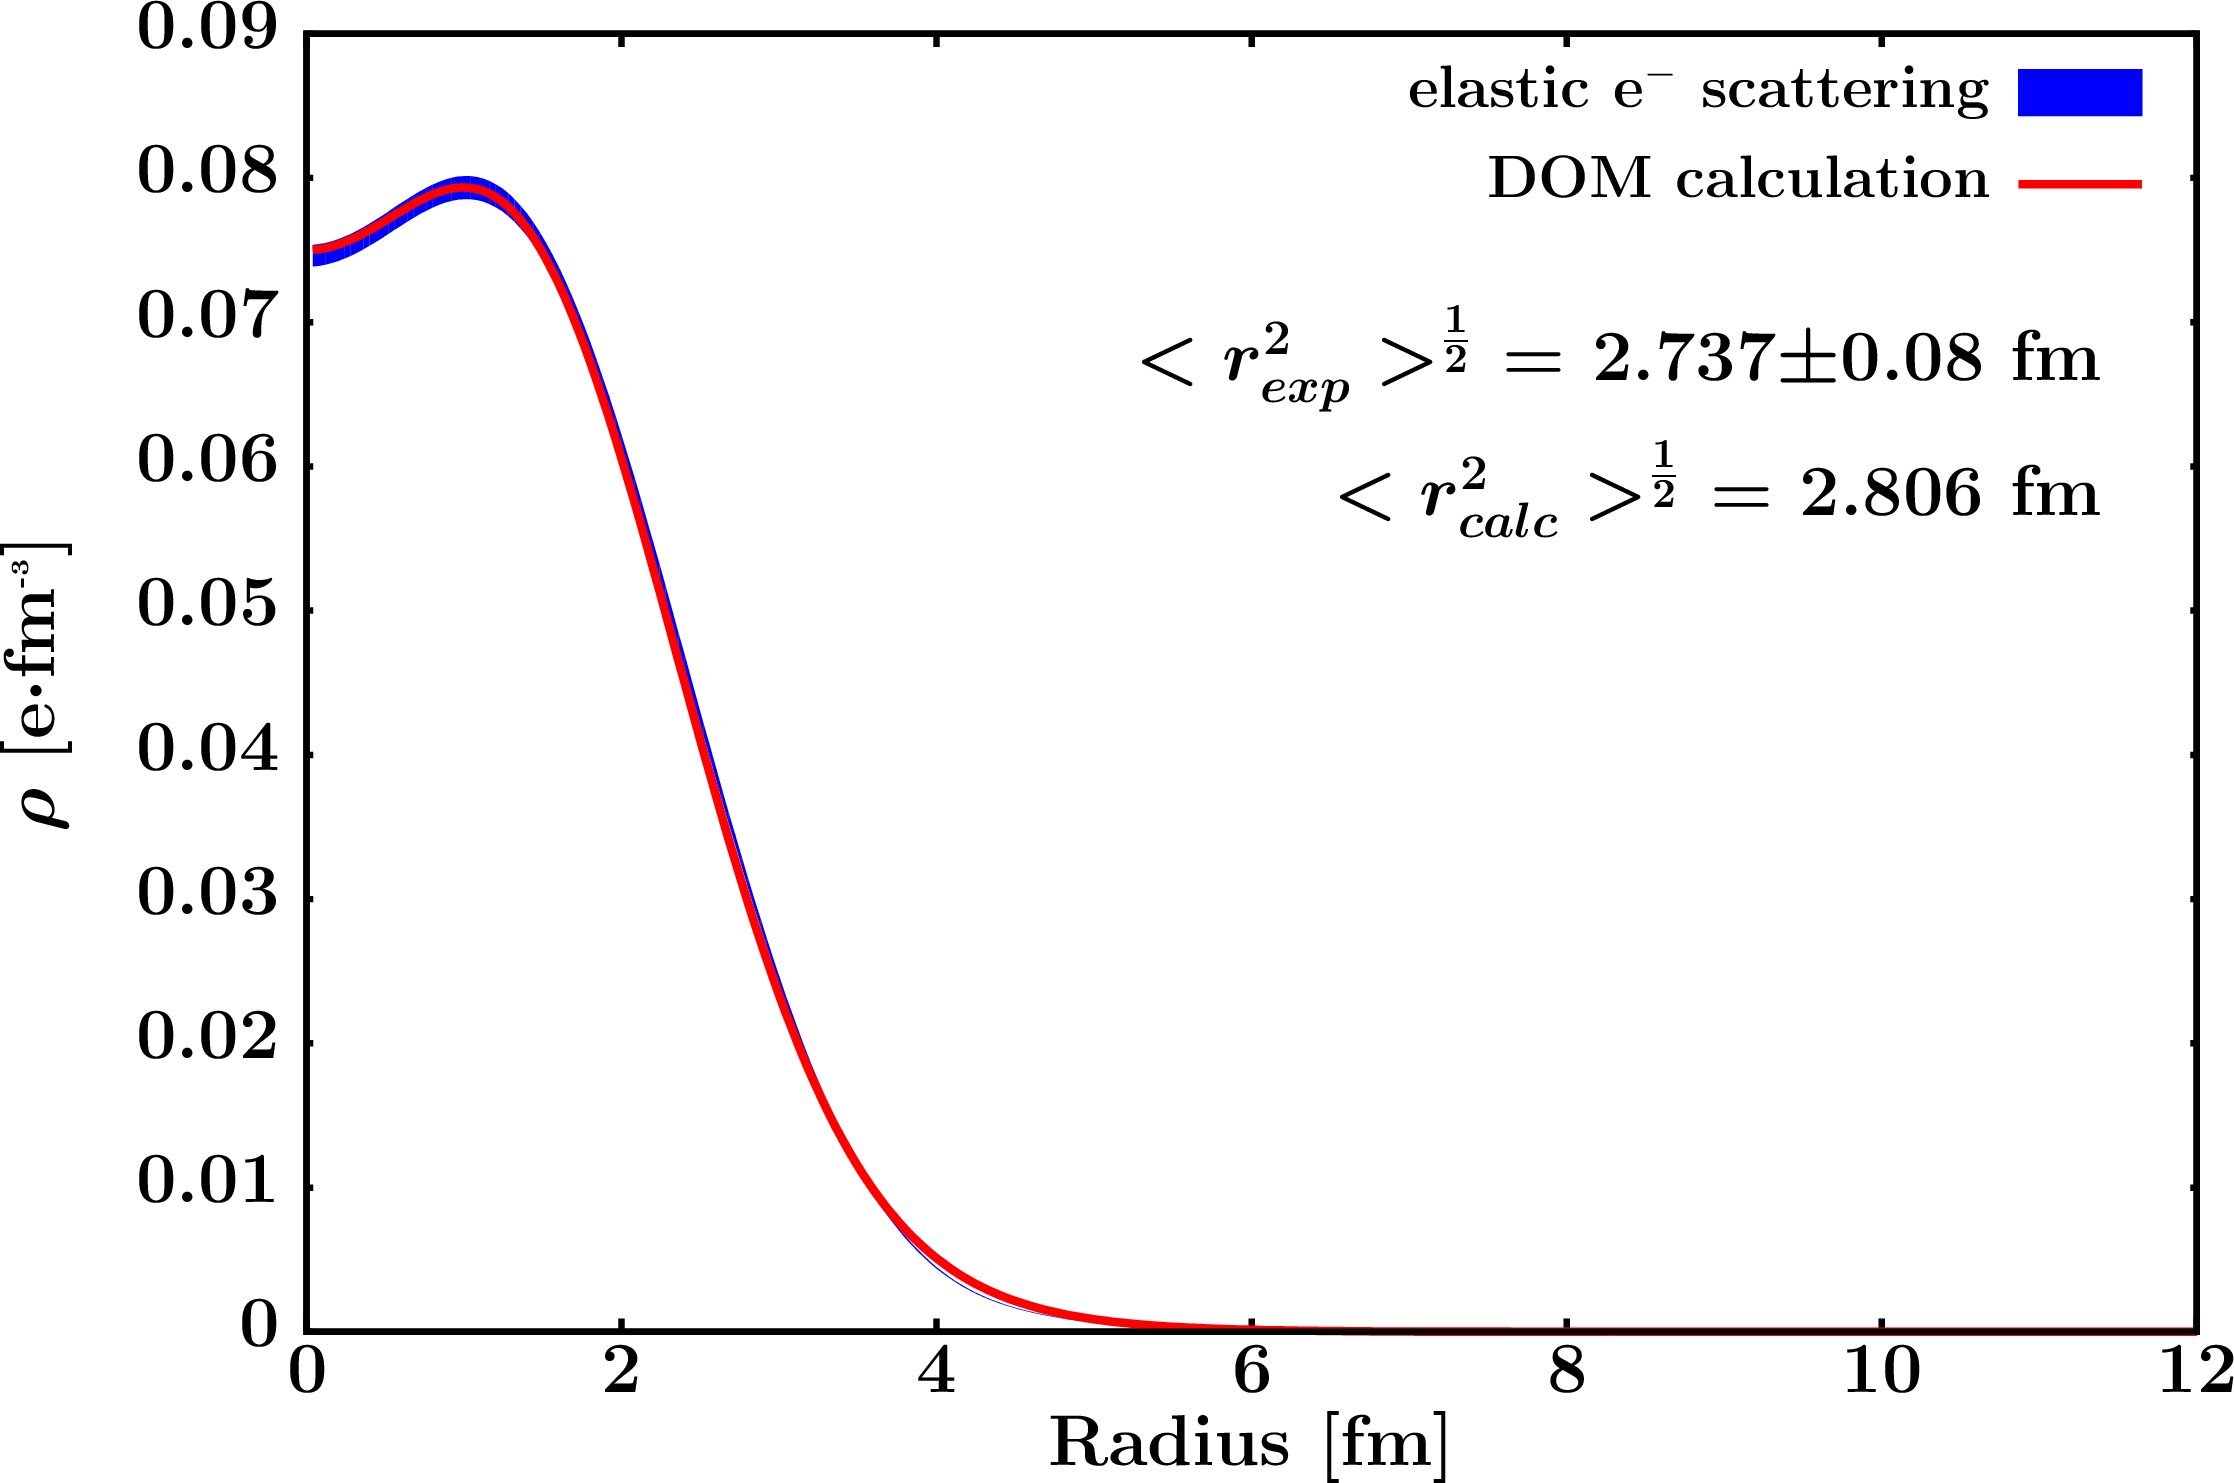
\includegraphics[width=0.75\textwidth]{figures/o16_chargeDensity.png}
    \caption[Proton single-particle density distributions in \oSix]
    {
        Charge density distribution of \oSix, as generated
        by our DOM fit (in red) and as generated from experimental
        elastic electron scattering \cite{DeVries1987}. No error bars are
        reported in the compilated of \cite{DeVries1987}; we show an
        arbitrary uncertainty range of 1\% (blue shaded region).
    }
    \label{o16ChargeDensity}
    \vspace{16pt}
    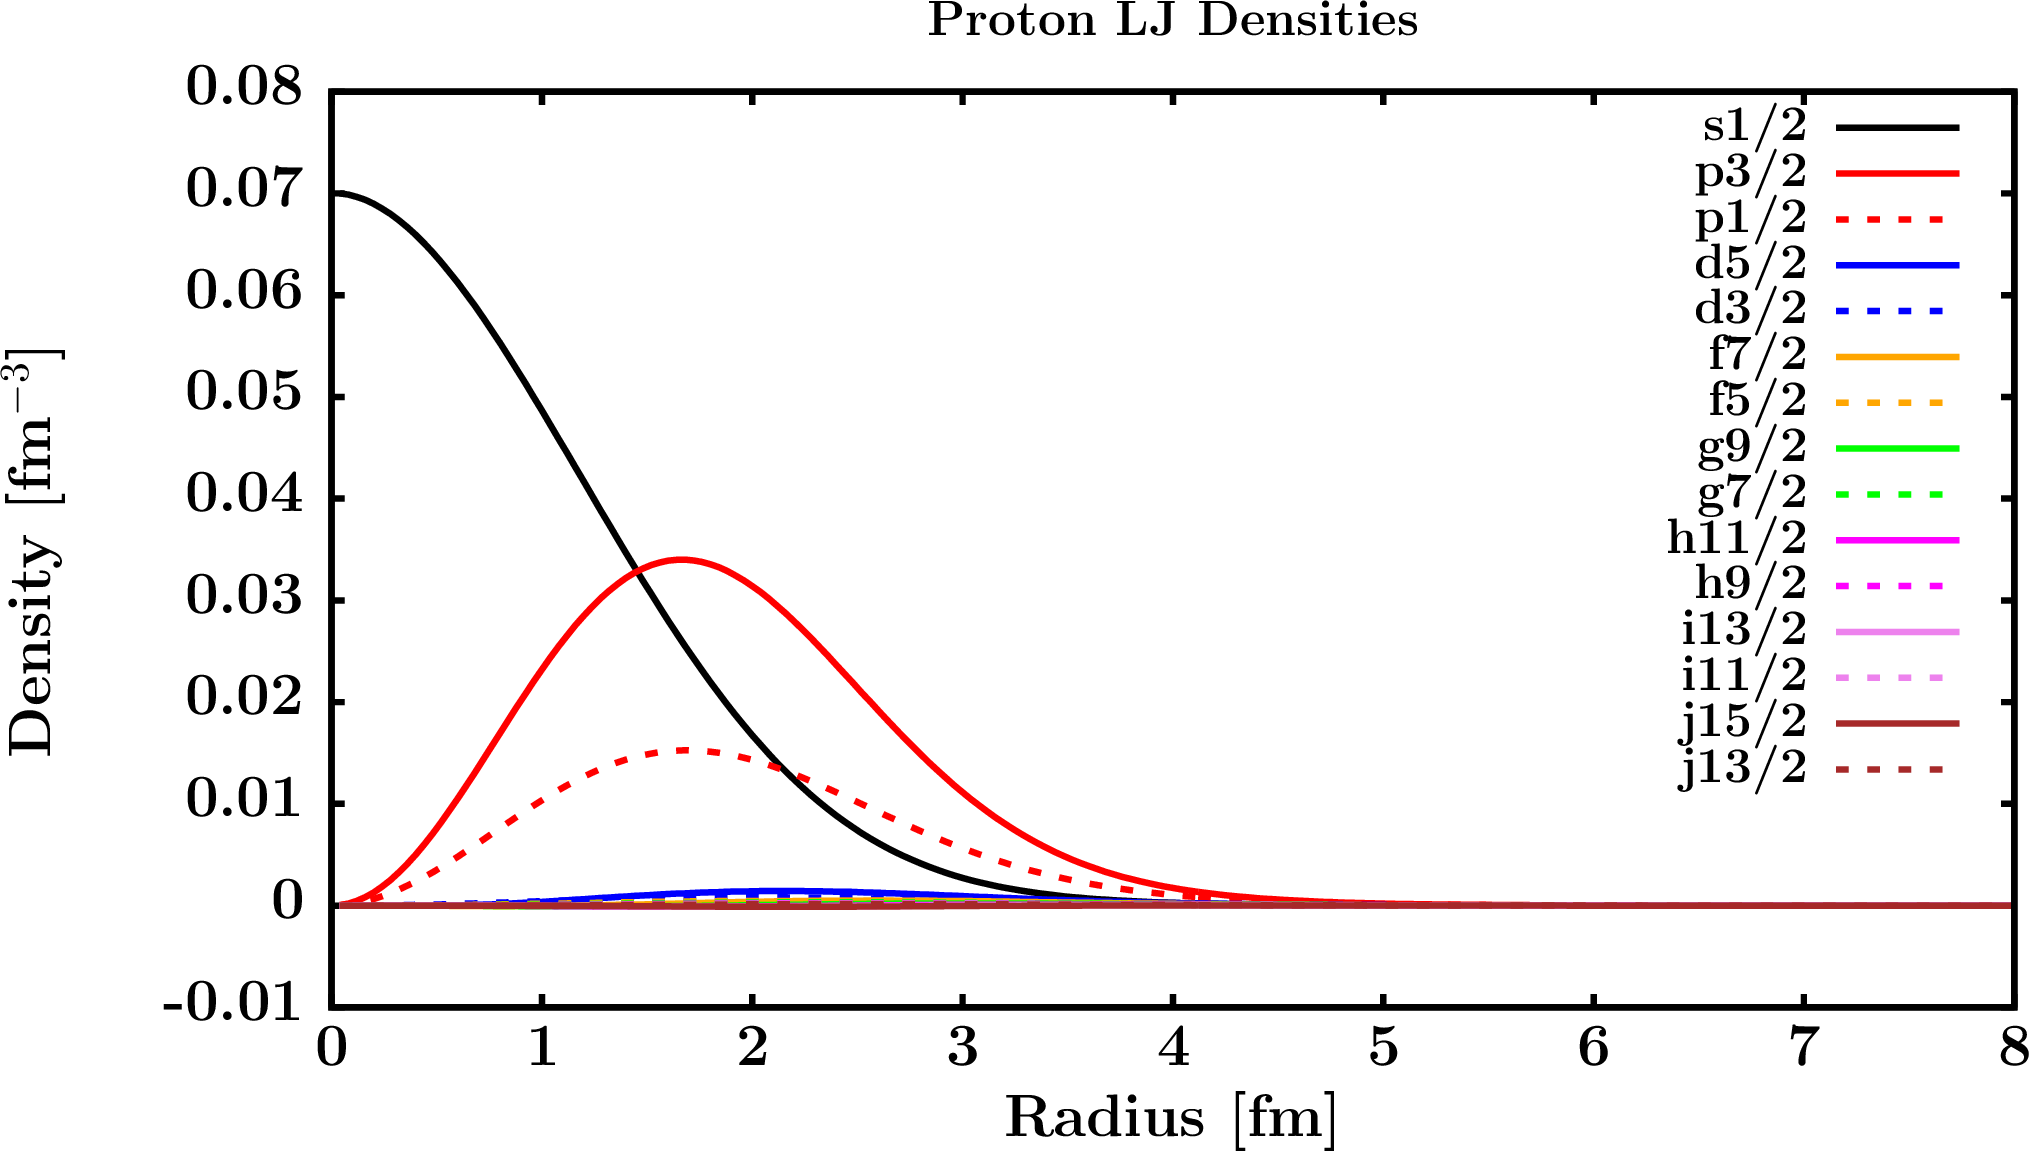
\includegraphics[width=0.75\textwidth]{figures/o16_protonLJDensityDist.png}
    \caption[Proton single-particle density distributions in \oSix]
    {
        Proton single-particle density distributions in \oSix, as generated
        by our DOM fit.
    }
    \label{o16LJDensityDist}
\end{figure}

%As with \caForty\ and \pbEight, (e,e'p) cross sections have been measured on \oSix. These data
%provide direct access to the momentum distribution of bound nucleons and are thus a critical test
%for the validity of our fits. Figure \ref{O16eep} presents the results of a calculation of (e,e'p)
%cross sections from the DWEEPY code \cite{Atkinson2018, Giusti2011} that uses the DOM potential and partial waves as input.
%It is important to note that these data were not used in the fitting of the DOM
%potential for \oSix\ and thus they give an indication of how well
%the DOM potential can be used for prediction rather than just reproduction of experimental data.
%
%\begin{figure}[tb]
%    \centering
%    \includegraphics[width=0.9\textwidth]{figures/O16eep.png}
%    \caption[\oSix\ (e,e'p) cross sections calculated by the DOM]
%    {
%        \oSix\ (e,e'p) cross sections calculated by the DOM (solid line) and experimental data from
%        \cite{Leuschner1994}.
%    }
%    \label{O16eep}
%\end{figure}

As with \caForty, we find that \oSix\ has a slightly negative neutron skin,
-0.024 \femto\meter.

\subsection{Results for \oEight}
For \oEight, a complete Fourier-Bessel-parameterized charge density distribution (used
for \oSix, \caAughtEight, \niEightFour, \snTwelve, and \pbEight) was unavailable. To
generate an approximate charge density distribution for \oEight\, we linearly
scaled the \oSix\ charge density distribution to reproduce
the \oEight-\oSix\ $\delta_{RMS}$
from \cite{DeVries1987} while maintaining a total charge of eight.
The reported RMS charge radii of \oSix\ and \oEight\ differ by only
0.07 fm ($\approx$2.5\%), so the \oEight\ charge density distribution
we generated is barely distinguishable from the \oSix\ distribution.
This same scaling procedure was also employed to
generate a charge density distribution for \snTwelve, using the
experimentally-derived \snFour\ charge density distribution.

To initiate the fit on \oEight, the \oSix\ best-fit parameter values
were assigned to the \oEight\ parameter file and observables were calculated to compare
with \oEight\ experimental data. The \oSix\ optimized parameter values
were moderately successful at reproducing
the \oEight\ scattering data without further adjustment, though almost no
neutron scattering data was
available for \oEight\ besides our newly-measured neutron \tot.
Using the raw \oSix\ parameters, the DOM predictions for
\oEight\ proton SP levels were underbound by several \mega\electronvolt\ per
particle and the calculated particle number was too low, unsurprising
given the insufficiency of the \oSix\ Hartree-Fock term in providing
two additional nucleons' worth of binding in \oEight. Thus, before
loosening any other parameters, the HF depth and HF depth asymmetry terms were allowed to vary,
reducing the chi-square contribution from the charge density, particle number, and energy level
sectors. Once a chi-square minimum had been reached with these two parameters, all other 
parameters were allowed to vary. Our optimum fit achieved good agreement with all
experimental \oEight\ scattering data except the 24 MeV neutron elastic scattering data
of Grabmayr et al. \cite{Grabmayr1980}, where our fit somewhat underestimates
the differential cross section throughout its range.

\begin{figure}[tb]
    \centering
    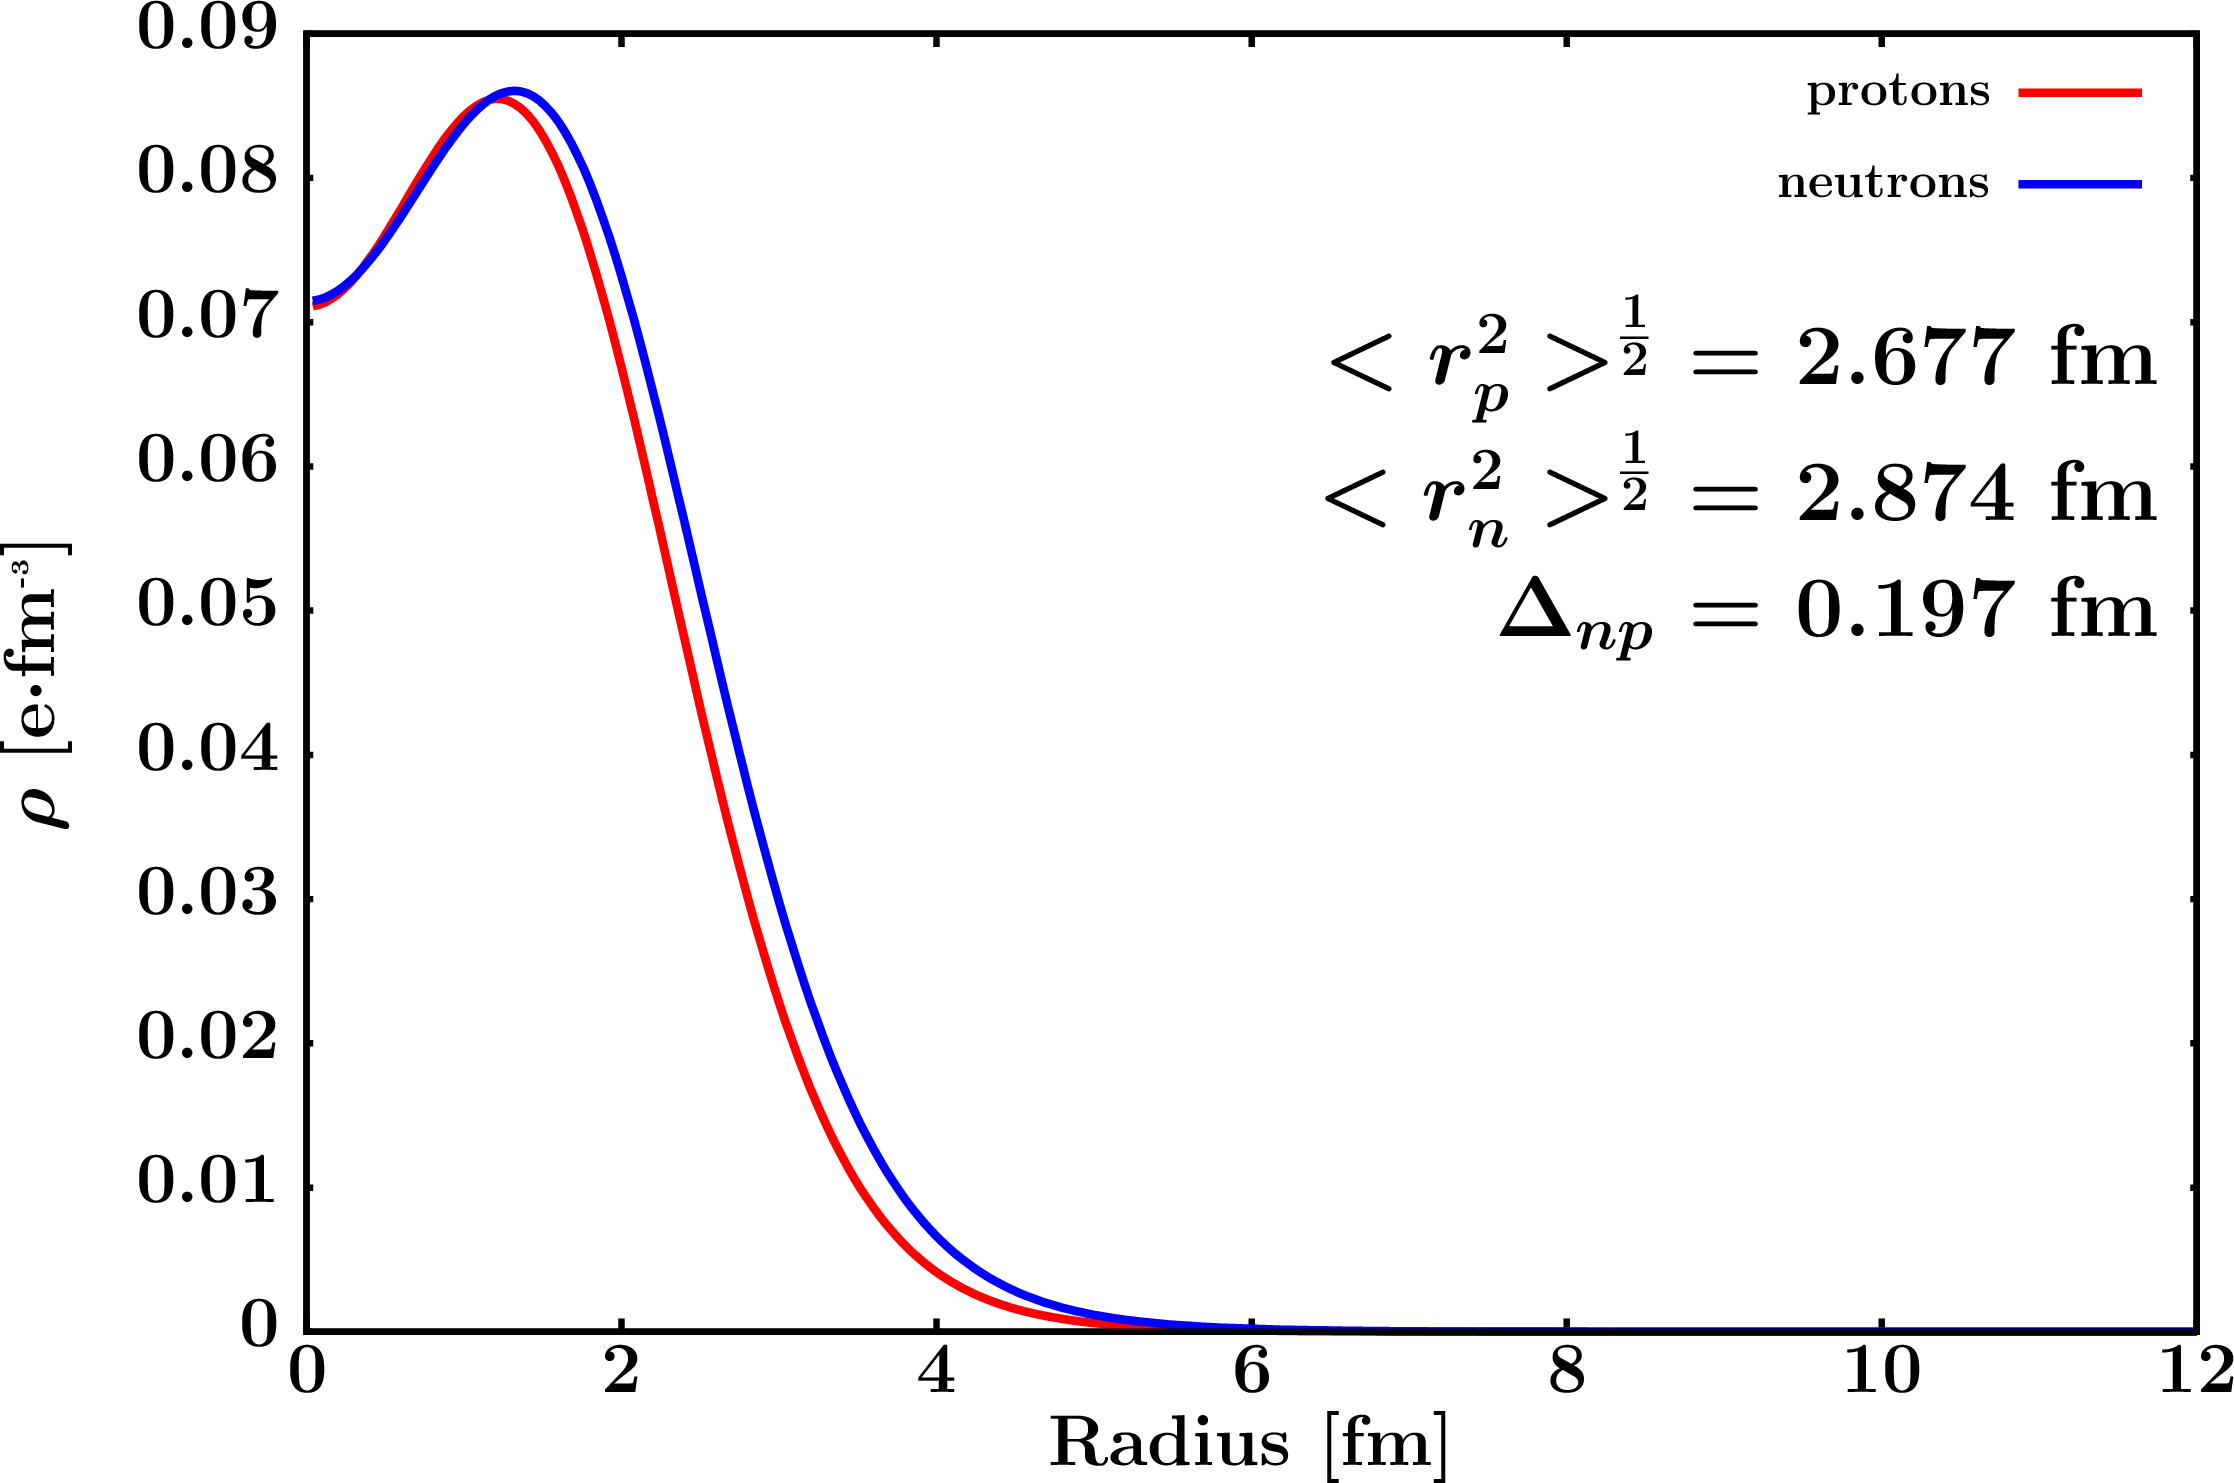
\includegraphics[width=\textwidth]{figures/o18_matterDensity.png}
    \caption[Proton and neutron matter density distributions in \oEight]
    {
        Proton and neutron point density distributions in \oEight, as
        generated by our DOM fit. The RMS radii of the distributions and their
        difference (the neutron skin) are provided. Adding two neutrons to \oSix\ dramatically
        increases the neutron skin, as most of the added neutron density settles into
        the $\nu$0\dFive\ shell, outside the \oSix\ core. A comparison to the
        experimental \oEight\ charge density distribution is shown in Section
        \ref{o18DOMOutput} of Appendix \ref{DOMVisualization}.
    }
    \label{O18MatterDistribution}
\end{figure}

Figure \ref{O18MatterDistribution} shows the matter density distributions for protons
and neutrons extracted from our fit on \oEight. We recover a large neutron skin of
0.197 \femto\meter, commensurate with the neutron skin of much heavier,
more asymmetric nuclei. The reason is clear: most
of density from the two extra neutrons in \oEight\ goes into the
$\nu$0\dFive, which peaks at the nuclear surface, increasing the neutron RMS
radius. To test our extracted neutron skin thickness for \oEight\, we considered 
the difference in RMS charge radii between mirror nuclei \neEight\ and \oEight.
The values of 2.97 \femto\meter\ for \neEight\ from \cite{Marinova2011} and
2.79 \femto\meter\ for \oEight\ from \cite{DeVries1987, Brown1979}
yield a difference of 0.18
\femto\meter, quite close to our extracted neutron skin for \oEight.

\section{Results for \niEightFour}
Unlike \caAughtEight, both \niEight\ and \niFour\ have partially-occupied neutron shells in the
independent-particle-model picture. Accordingly, Ni isotopes have increased level density near the
Fermi level and should possess significant imaginary strength in this region, impacting
low-energy elastic and inelastic nucleon cross sections. Recently, A. Brown has outlined a
program to constrain the density dependence of the symmetry energy using RMS charge radii in mirror
nuclei in the Fe and Ni region \cite{Brown2017}, heightening interest in accurate
matter density distributions for these isotopes. While \niSixty\ and \niTwo\
were not analyzed here, the charge density distributions of
both are well-known \cite{DeVries1987}, making the even Ni isotopes an ideal target for a future
DOM analysis along an isotope chain.

\subsection{Results for \niEight}
Like \caForty, \niEight\ enjoys abundant proton and neutron elastic scattering data.
In our \niEight\ fit, the imaginary strength rises steeply just above the Fermi energy,
understandable in light of the lower-lying excited states in \niEight\ compared to all the lighter
closed-shell isotopes already presented. As with \caEight, the lack of high-energy proton \rxn\ data
makes it difficult to unambiguously identify the high-energy imaginary strength ($W_{vol}^{+}$).

\begin{figure}[tb]
    \centering
    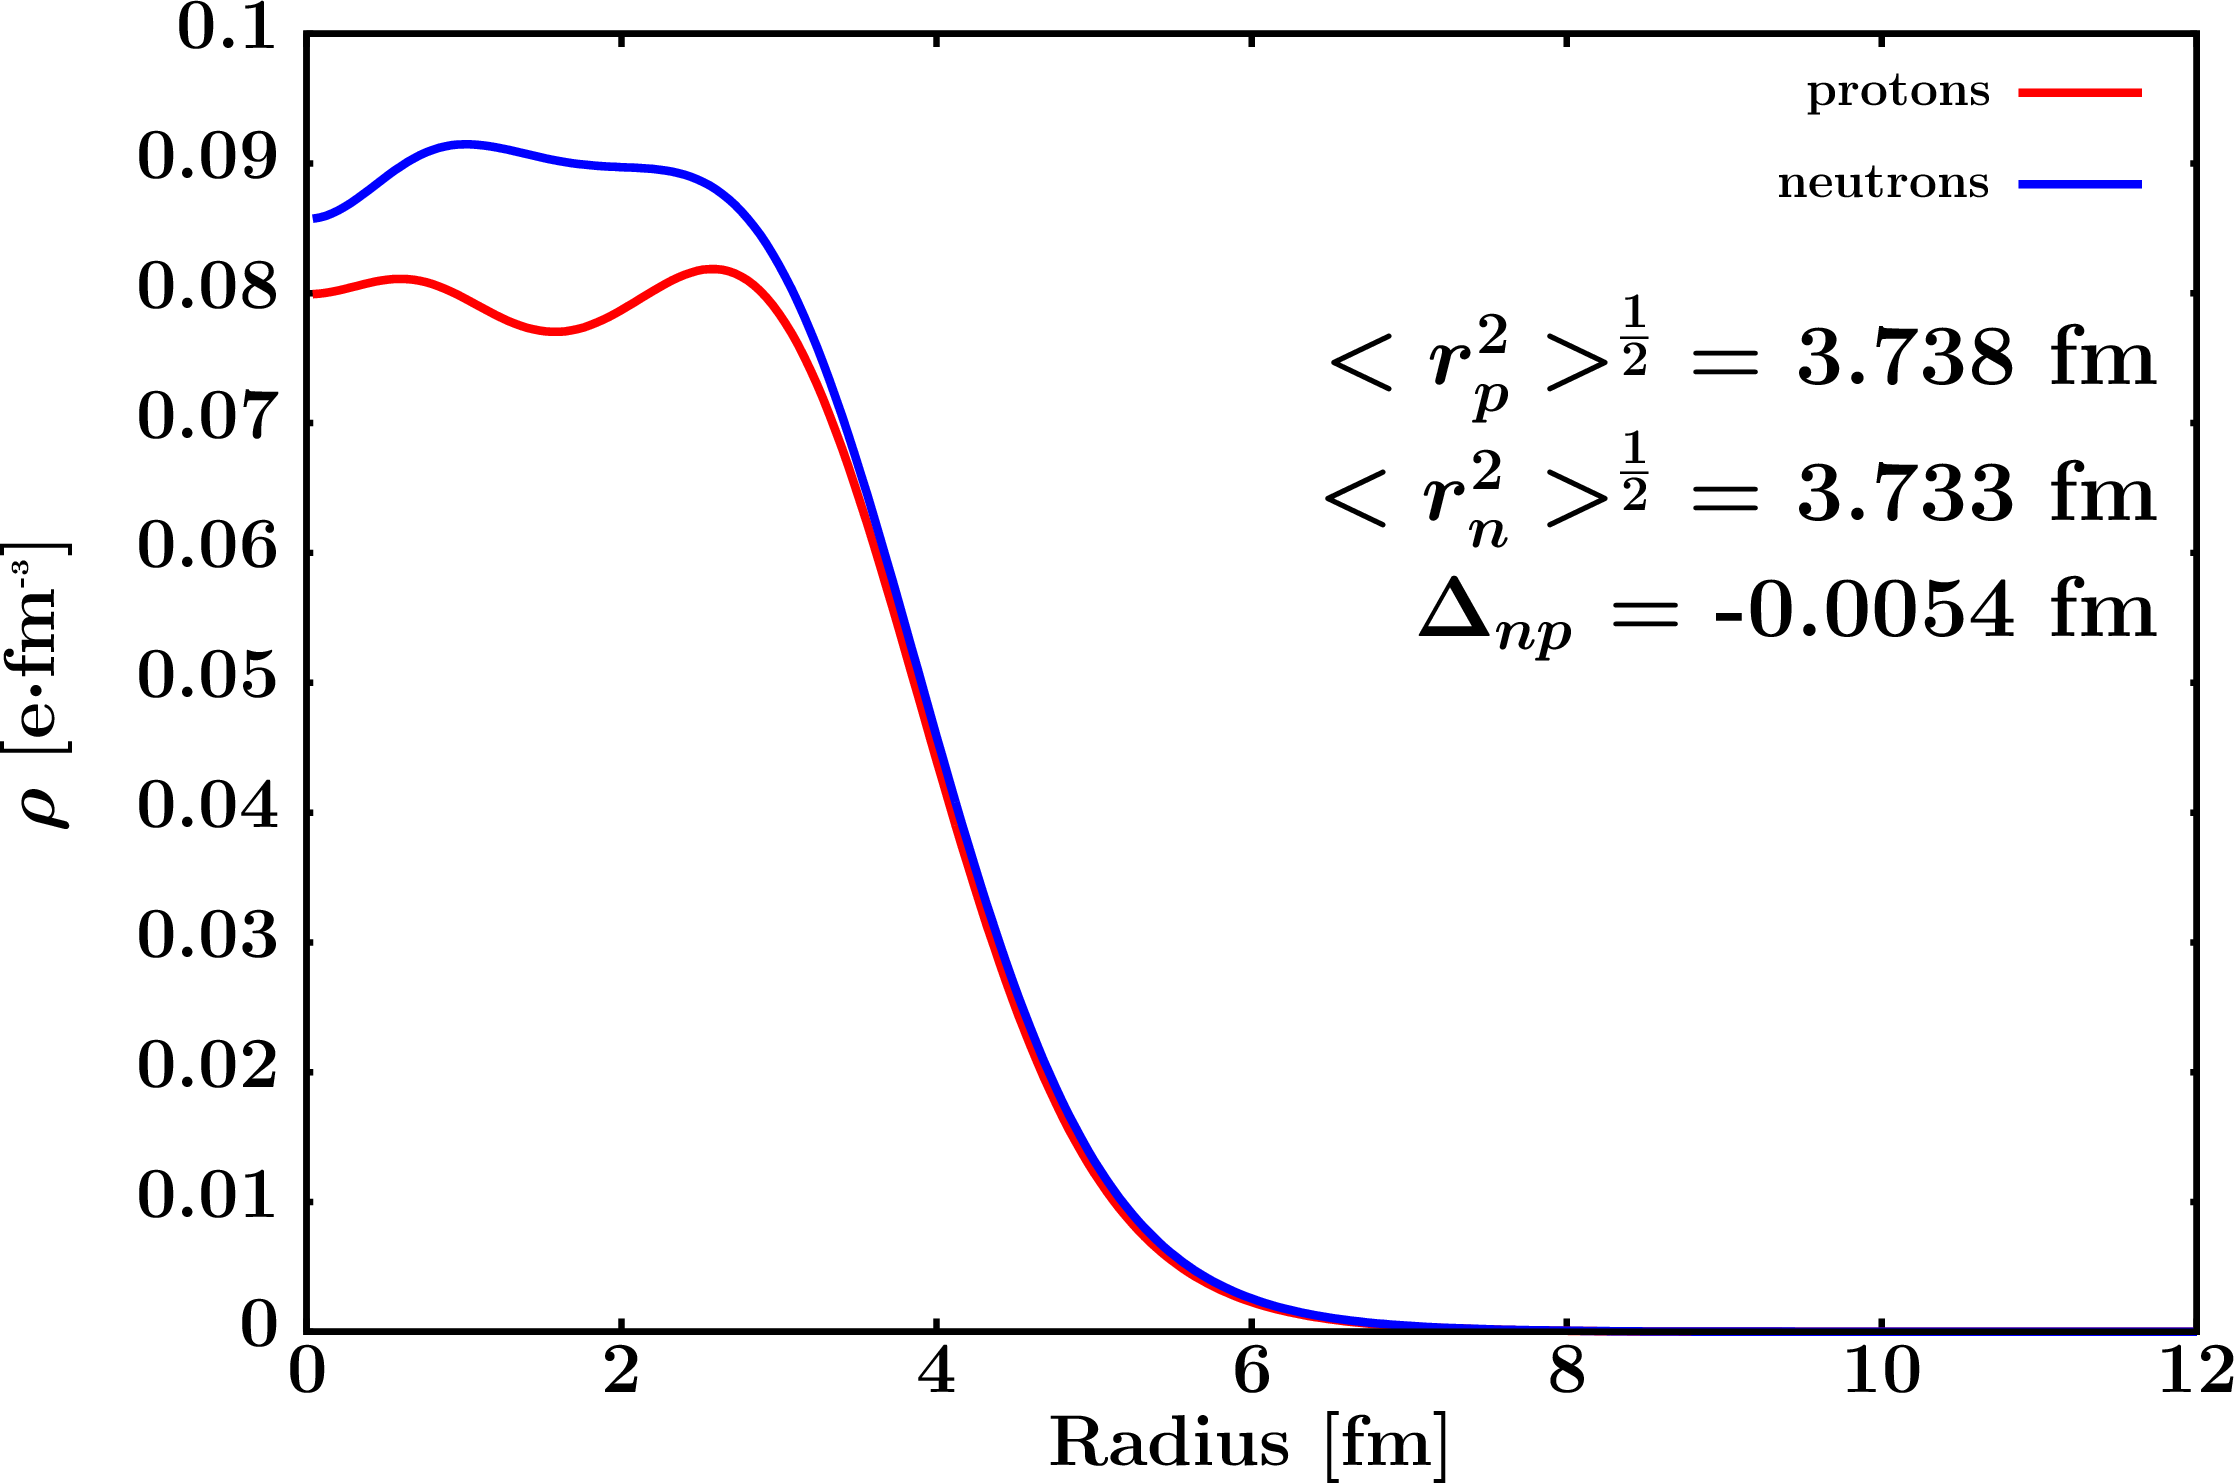
\includegraphics[width=\textwidth]{figures/ni58_matterDensity.png}
    \caption[Proton and neutron matter density distributions in \niEight]
    {
        Proton and neutron point density distributions in \niEight, as
        generated by our DOM fit. The RMS radii of the distributions and their
        difference, the neutron skin, are provided. The two valence neutrons (with respect to
        a \niSix\ core) do little to increase the neutron skin, as most of the added
        neutron density populates the $\nu$1\pThree\ shell close to the nuclear core.
        A comparison to the
        experimental \niEight\ charge density distribution is shown in Section
        \ref{ni58DOMOutput} of Appendix \ref{DOMVisualization}.
    }
    \label{ni58MatterDistribution}
\end{figure}

Figure \ref{ni58MatterDistribution} shows the matter distributions and neutron skin we extract for 
\niEight. In the case of \oEight, the addition of two neutrons compared to symmetric \oSix\
increased the neutron skin size dramatically. In \niEight, the two extra neutrons (with respect to
symmetric \niSix) join the p-shell, dwelling mostly near the nuclear core where they do little
to change the neutron skin size. Per this rudimentary picture, it is clear that
shell structure is critical for understanding the evolution of neutron skins along an isotope chain. 

\subsection{Results for \niFour}
Due to its low natural abundance, \niFour\ is a dramatically more expensive target material than
\niEight, making experimental coverage very sparse on this isotope. Our search
of the EXFOR database showed
no \niFour\ elastic or inelastic neutron scattering data at all, except for a single study on
$^{58,60,62,64}$Ni from 5-7 MeV almost forty years old \cite{Korzh80}.
Without our new \tot\ data, a DOM analysis of this type would have been infeasible. Our
fit of \niFour\ easily converged on our new neutron \tot\ and the
experimental binding energy per nucleon, suggesting
that the \niFour\ fit parameters are still
significantly underconstrained. Accordingly, the neutron skin
we extract for \niFour\ is expected to be less
reliable but still worth reporting. Compared to \niEight, our fit suggests that much of the extra 
neutron density of \niFour\ adds to the occupation
of the $\nu$0\fSeven\ and $\nu$0\fFive\ subshells. 
The extra occupation in the high-angular-momentum f-shell grows the neutron
skin substantially, to 0.15 \femto\meter\ (cf. -0.0054 \femto\meter\ for \niEight).

\section{Results for \snTwelveFour}
Of the isotopic systems studed in this treatment, \snTwelveFour\ was the least characterized with 
experimental data. Our new neutron \tot\ and \el\ measurements provide a sizable fraction
of the total available nucleon scattering data on \snTwelveFour\ from 1-200 \mega\electronvolt.
Because of the lack of data, our Sn fits are likely the least well-constrained of all the fits
presented here, with the possible exception of \niFour.
Still, the structural information exctracted from
our fits on \snTwelveFour\ largely comports with the trends seen in the other isotopic systems and
may be useful for extrapolating properties of the doubly-magic $^{100}$Sn and
$^{132}$Sn. In addition, mid-shell Sn isotopes exhibit neutron superfluidity
and help provide important information
about deviations from the shell model outside shell closures. 

\subsection{Results for \snTwelve}
For \snTwelve, the only neutron scattering data available from 10-200 MeV were the new data sets
presented earlier in this work. Given this situation, it is encouraging that the momentum
distributions we extract, shown in Figs. \ref{sn112ProtonMomentumDistInt} and
\ref{sn112NeutronMomentumDistInt}, are comparable to those of both the
lighter \niEight\ and heavier \pbEight, suggesting that our parameters for \snTwelveFour\ are
reasonably well-constrained.
\begin{figure}[tb]
    \centering
    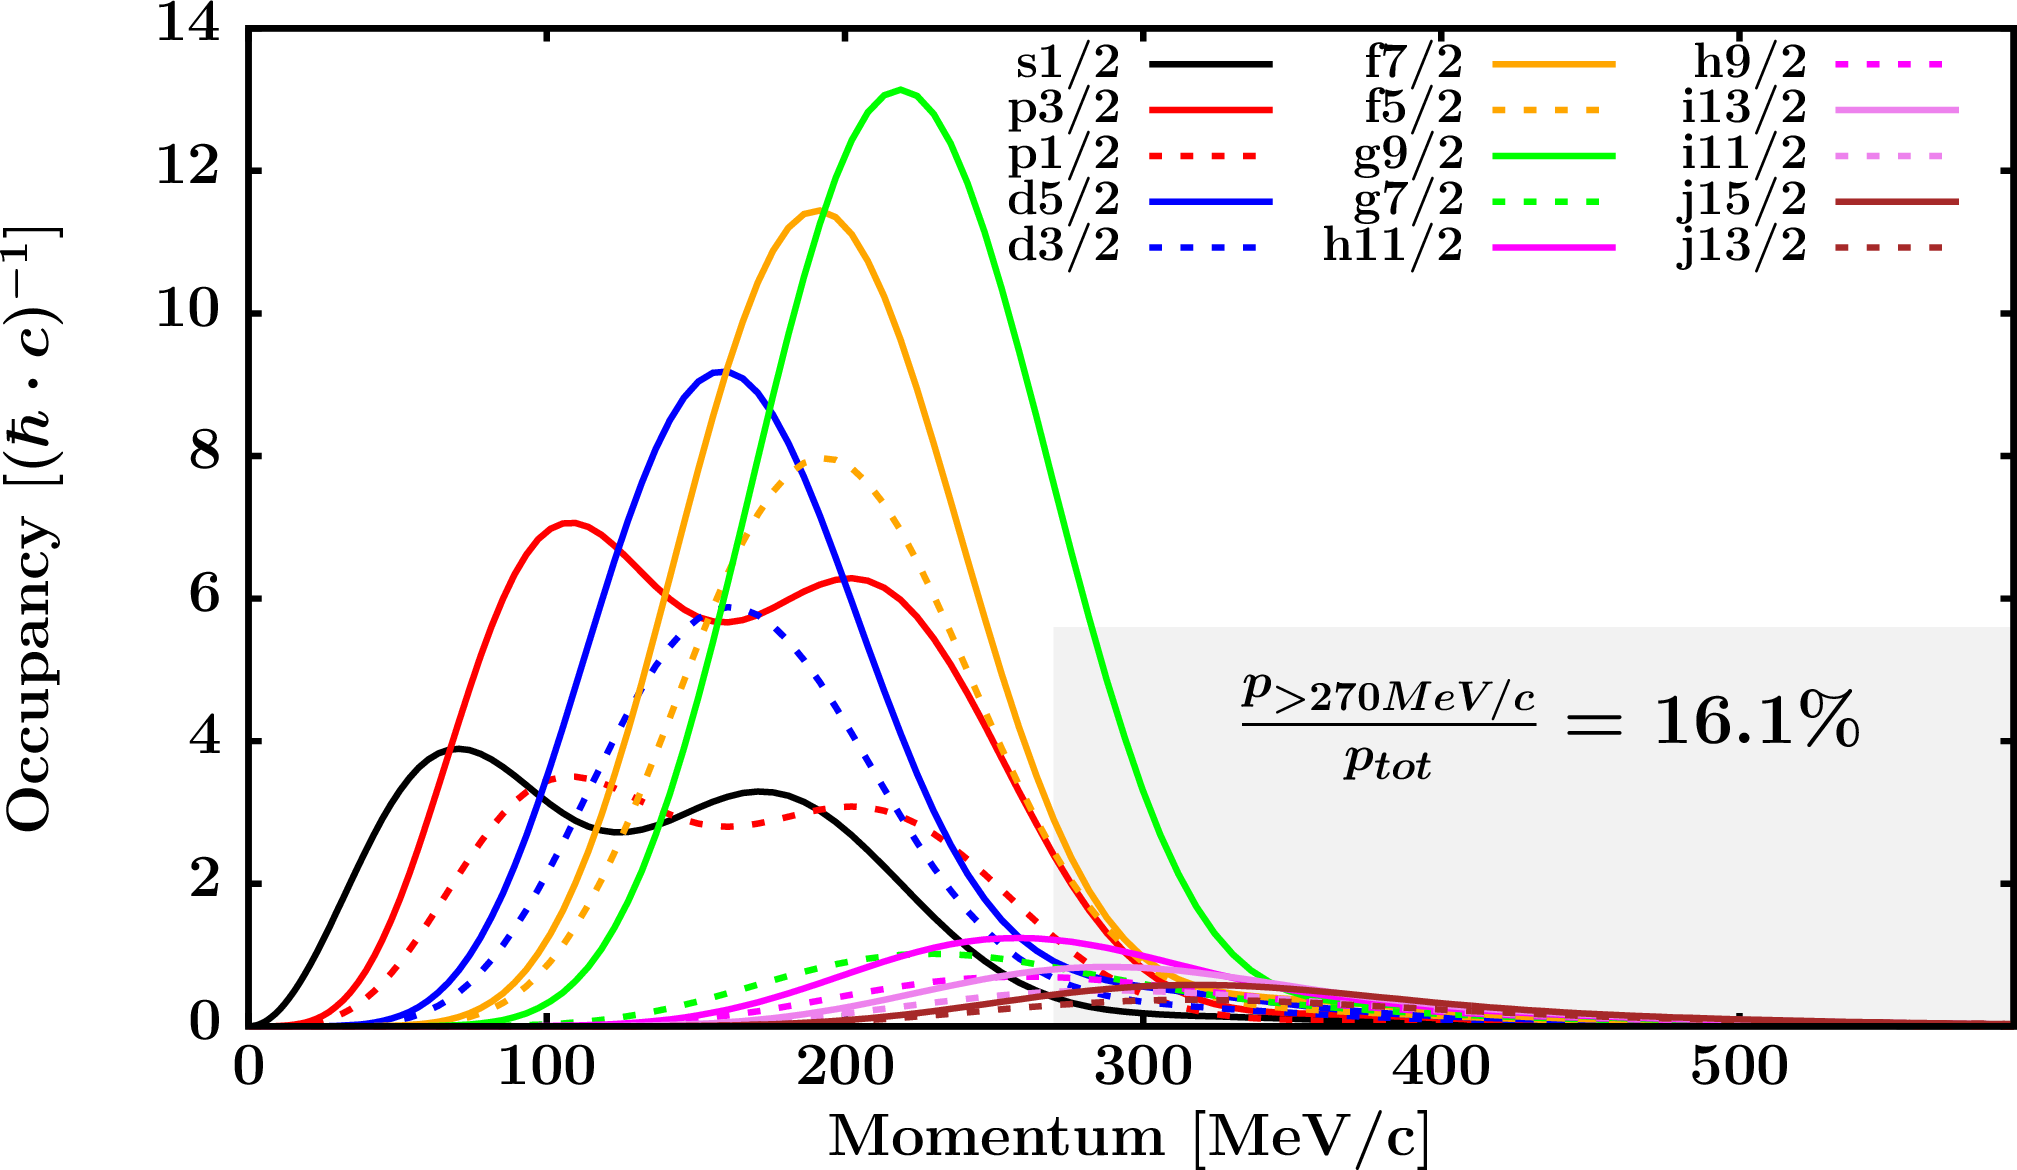
\includegraphics[width=0.75\textwidth]{figures/sn112_protonLJMomentumDistIntegral.png}
    \caption[Proton momentum distribution in \snTwelve]
    {
        Integrated proton momentum distribution in \snTwelve, as generated
        by our DOM fit. The fraction of proton high-momentum content is
        comparable, but slightly lower than, that of neutrons (figure below).
    }
    \label{sn112ProtonMomentumDistInt}
    \vspace{16pt}
    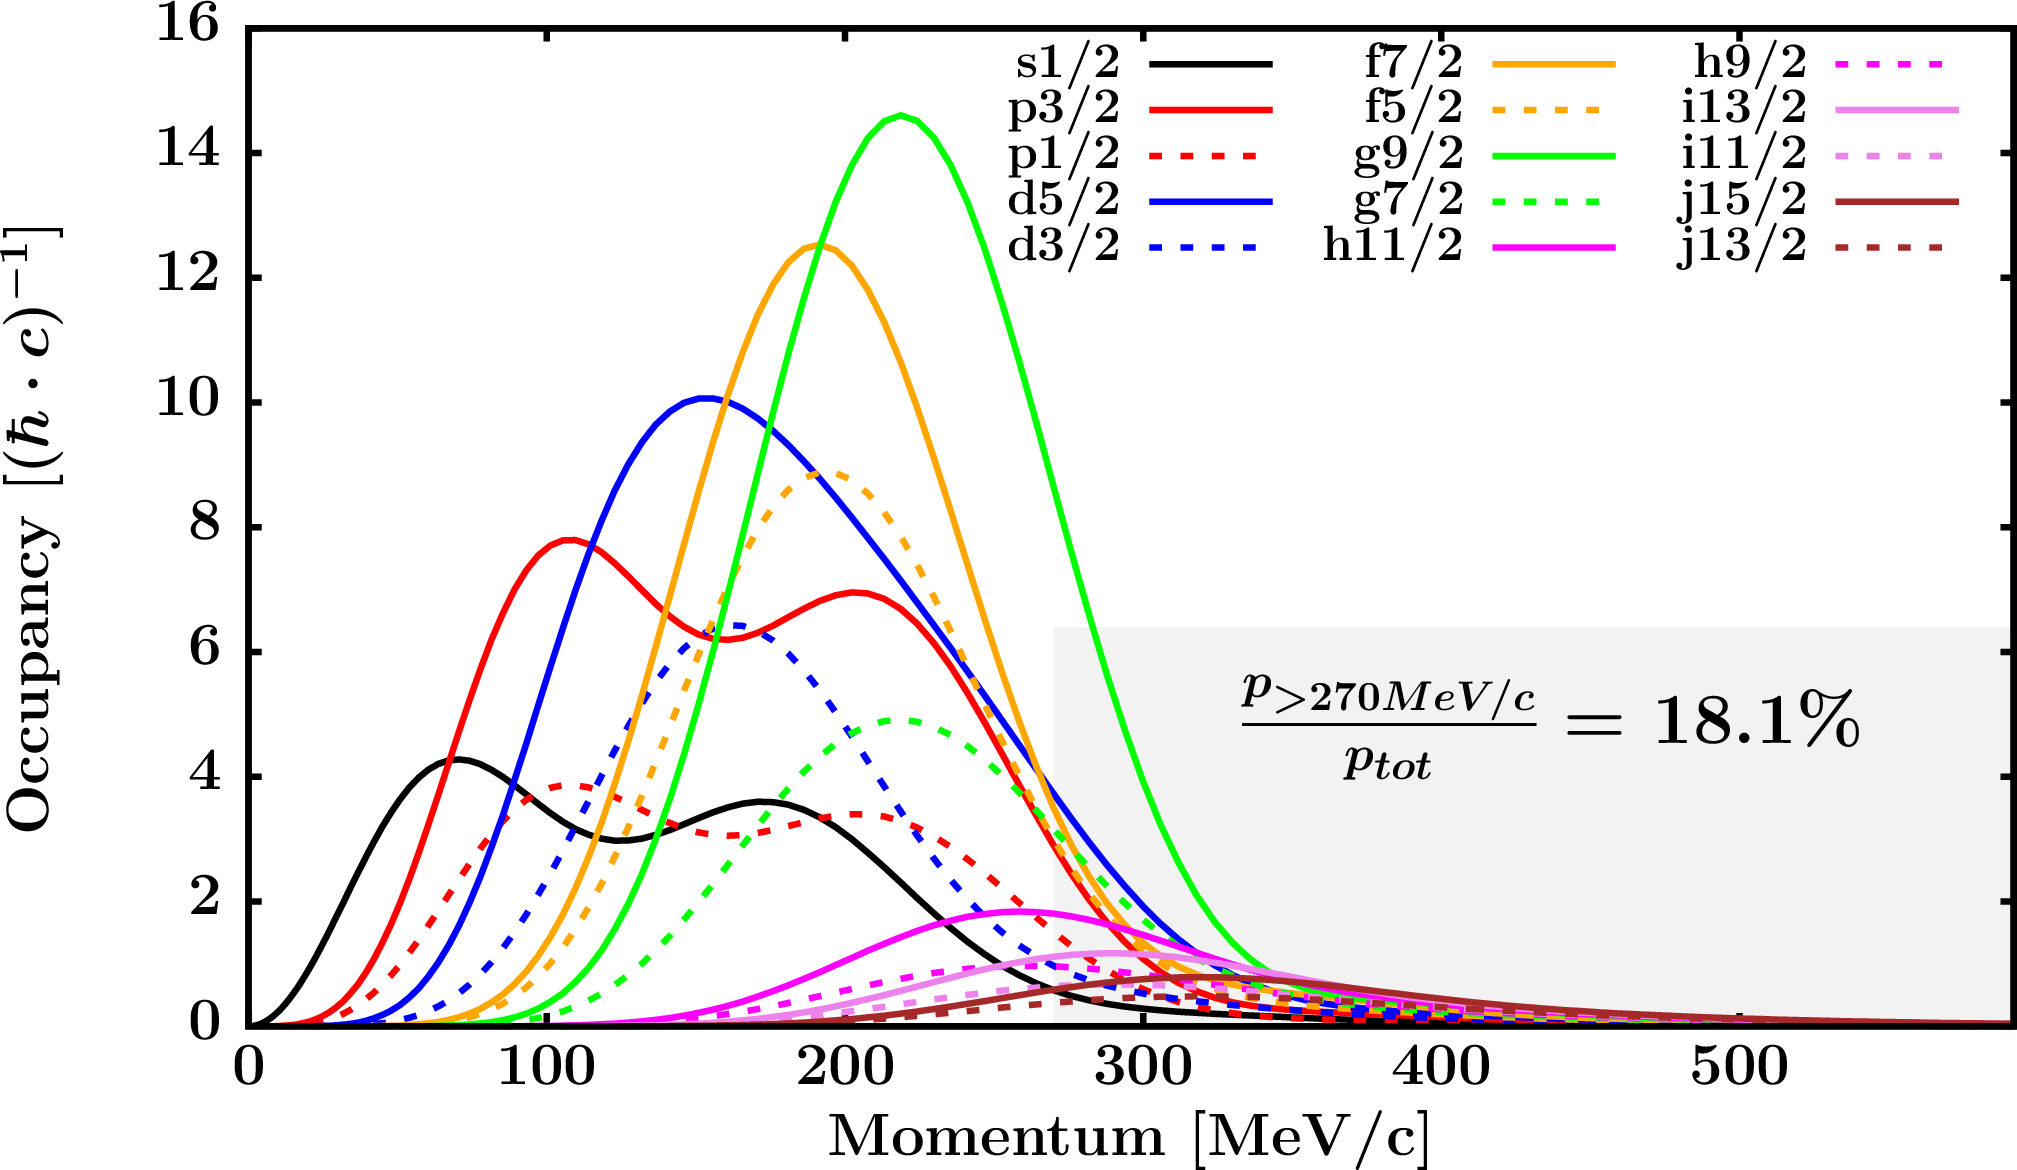
\includegraphics[width=0.75\textwidth]{figures/sn112_neutronLJMomentumDistIntegral.png}
    \caption[Neutron momentum distributions in \snTwelve]
    {
        Integrated neutron momentum distribution in \snTwelve, as generated
        by our DOM fit. The fraction of neutron density with
        momentum above 270 $\mega\electronvolt/\text{c}$ is listed.
    }
    \label{sn112NeutronMomentumDistInt}
\end{figure}

It should be noted that while \snTwelve\ and \oEight\ have almost the same asymmetry
($\frac{N-Z}{A}$), the valence neutrons in \snTwelve\ are spread more evenly over several
shells, so the neutron skin we recover is small.

\subsection{Results for \snFour}
Figure \ref{Sn124MatterDistribution} shows the matter distribution for protons and neutrons in
\snFour\ and the neutron skin as generated by our fit.
\begin{figure}[tb]
    \centering
    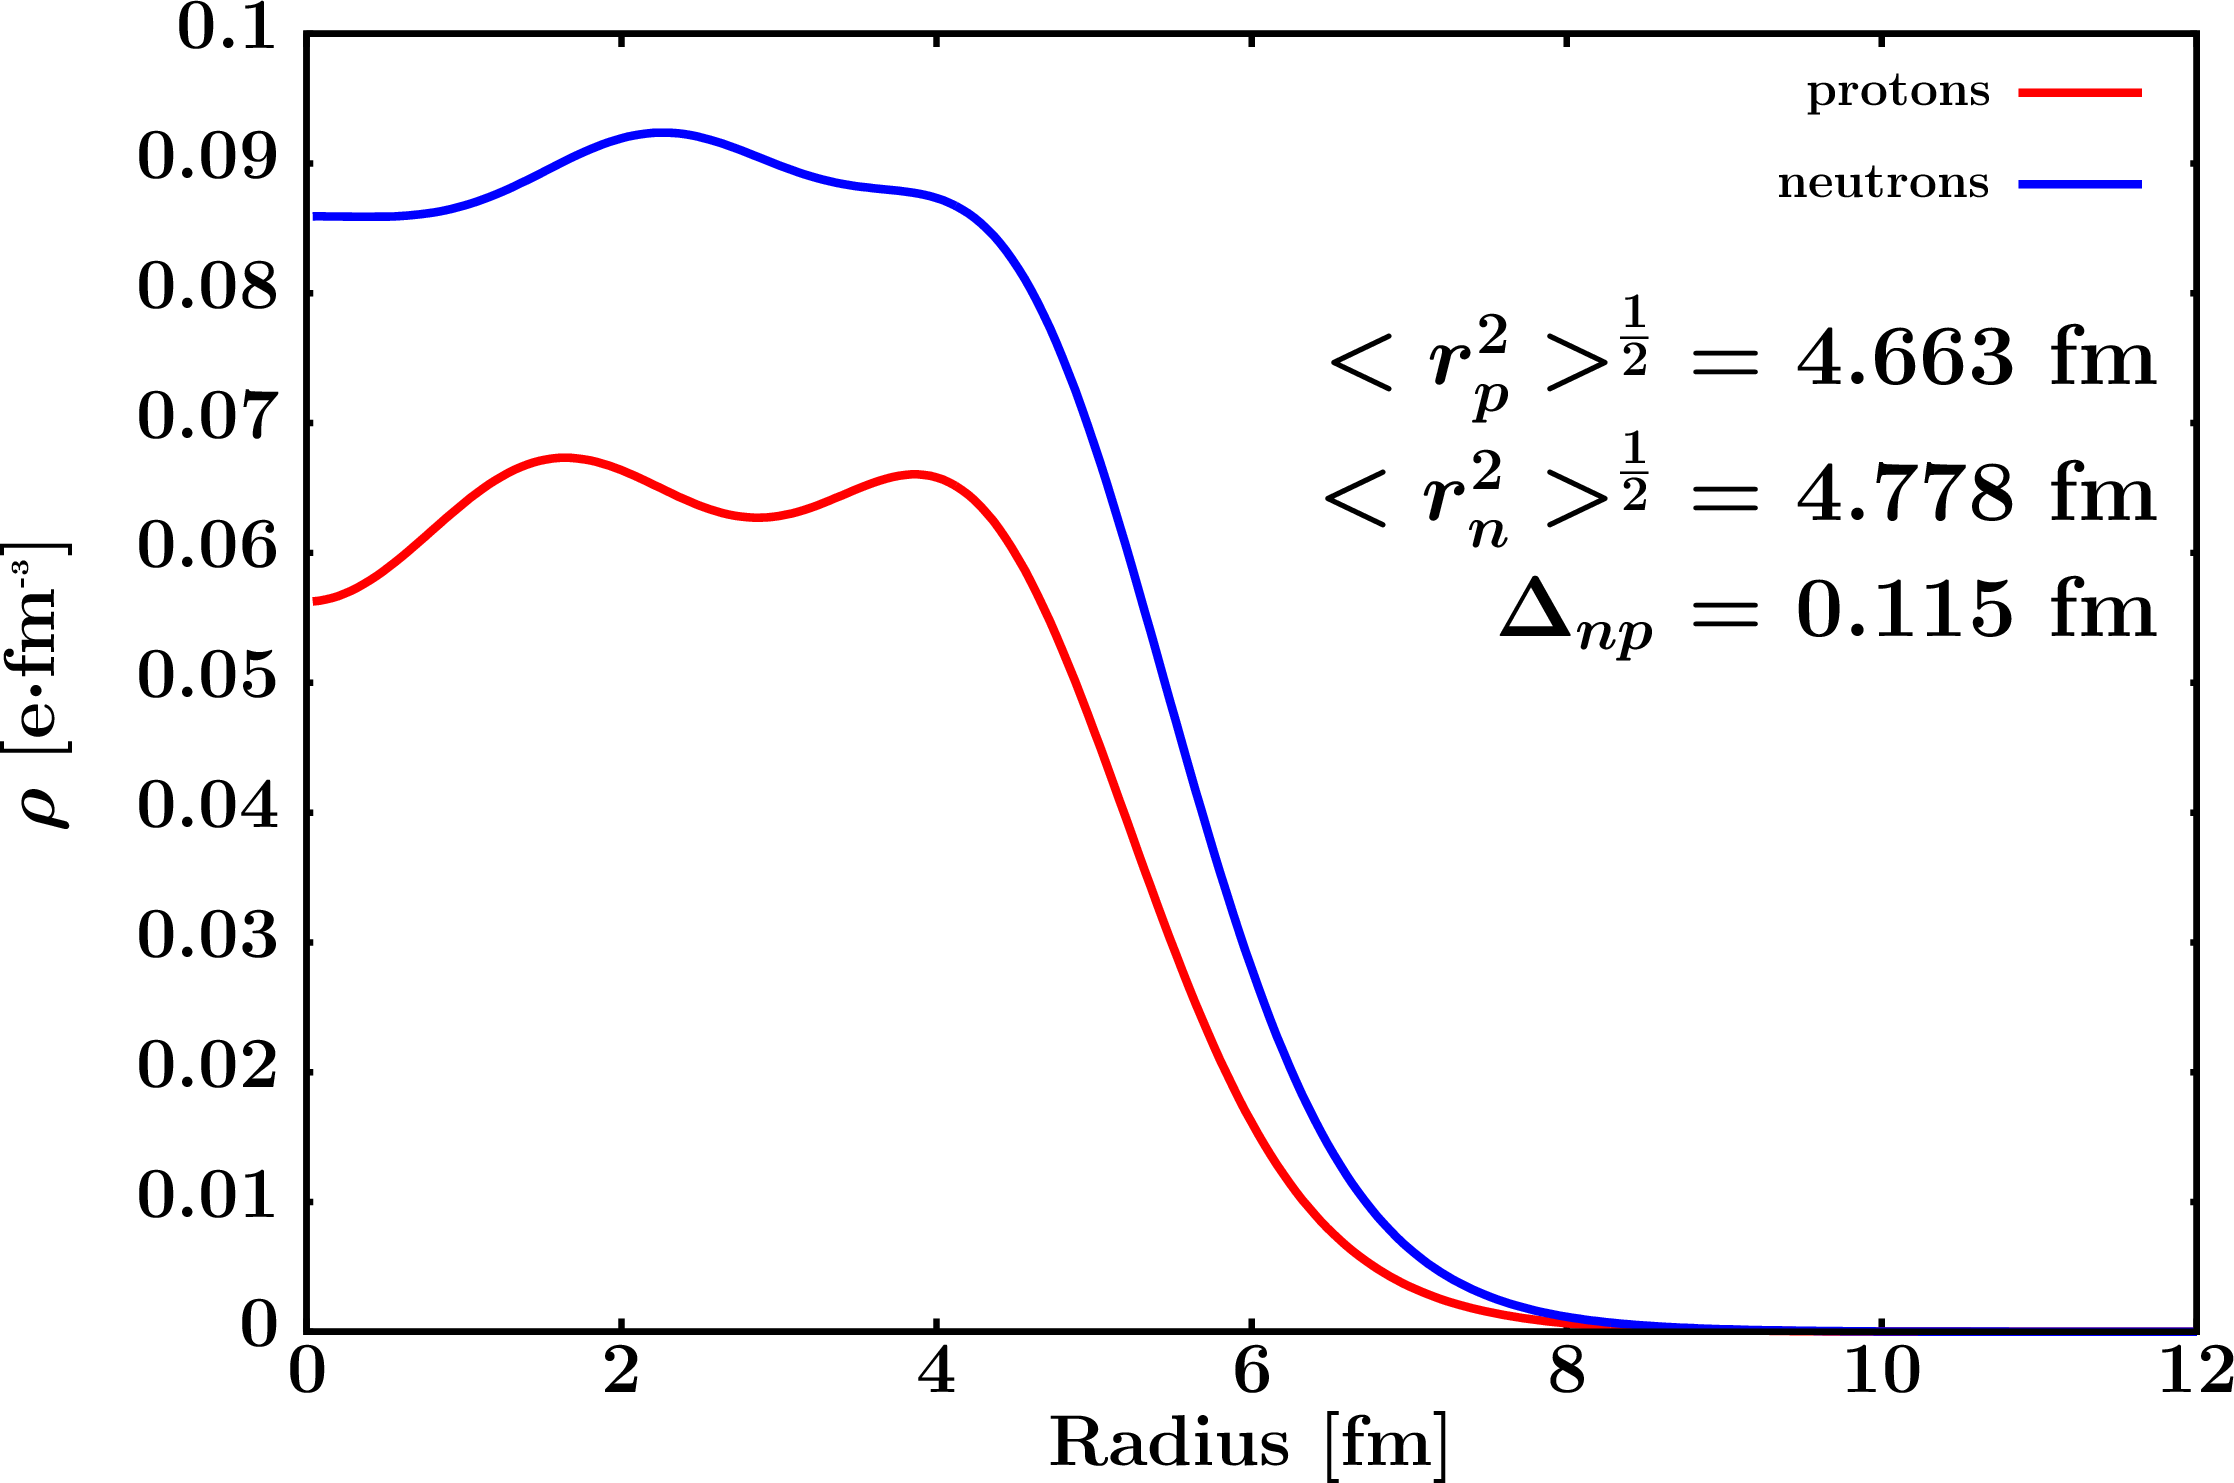
\includegraphics[width=\textwidth]{figures/sn124_matterDensity.png}
    \caption[Proton and neutron matter density distributions in \snFour]
    {
        Proton and neutron point density distributions in \snFour, as
        generated by our DOM fit. The RMS radii of the distributions and their
        difference (the neutron skin) are provided. The neutron skin of
        neutron-rich systems like \snFour\ are expected to be strongly correlated
        with the size of the density-dependence of the symmetry energy, $L$.
    }
    \label{Sn124MatterDistribution}
\end{figure}
For both Sn isotopes, we had trouble
reproducing the experimentally-derived charge density distributions with
the same degree of accuracy as the nuclei presented above.
Whether this difficulty stemmed from insufficient nucleon scattering
data or from a deficiency in our parameterization, we do not know. To make up for the lack of data
on any one Sn isotope, previous local DOM fits on the Sn isotopes \cite{Charity2006, Mueller2011}
had fit several members of the ten stable Sn isotopes simultaneously.
The current non-local DOM version used in this work is not equipped for this strategy, but it is a
promising direction that we hope to pursue in future work.

\section{Results for \pbEight}
Like \caForty\ and \oSix, \pbEight\ occupies an important square on the chart of nuclides and has
received a great deal of experimental and theoretical attention. 
The size of the neutron skin of \pbEight\ has been identified by numerous studies as highly
correlated with the density-dependence of the symmetry energy, $L$, a critical input for the neutron
star equation-of-state. By employing parity-violating electron scattering to probe the
weak charge distribution in \pbEight, the PREX experiment at Jefferson Laboratory extracted a
\pbEight\ neutron skin value of 0.33$\pm$0.17 fm. A followup experiment with improved statistics, PREX II,
is slated to run later in 2019, and is expected to provide a model-independent
value for the \pbEight\ neutron skin thickness to
within 0.06 fm. Given the wide range of \pbEight\ neutron skin thicknesses
predicted by relativistic
and non-relativistic mean-field models, this quantity is an excellent
test for the value of the DOM as a predictive tool.

Figures \ref{pb208ProtonMomentumDistInt} and \ref{pb208NeutronMomentumDistInt} show the momentum 
distribution for protons and neutrons we extract from
our \pbEight\ fit. As expected, the high momentum content is slightly larger than that for the Sn
isotopes. As with \caEight, the proton high-momentum content is lower than the
neutron high-momentum content, a consequence of additional filling of
higher-angular-momentum subshells for neutrons compared to protons, skewing the
total momentum distribution upward.
Figure \ref{Pb208MatterDistribution} shows the nucleon matter distributions, which yield a
neutron skin of 0.200 \femto\meter. Compared to
previous DOM treatments, our value for the
\pbEight\ neutron skin is slightly smaller and more in line with the average of mean-field
calculations \cite{Fattoyev2012}. An important difference in our DOM treatment is that only the
depth of the Hartree-Fock potential is allowed to vary with asymmetry; previous treatments
relaxed this restriction and equipped every real-term parameter with an asymmetry-dependence. We
suspect that some of the difference in our extracted \pbEight\ radii derives
from this choice. Unfortunately, our present fit of \pbEight\ fails to recover
enough binding energy per nucleon and substantially underbinds the most deeply-bound proton
levels (e.g., the 0\pThree), indicating that our description of very deep levels
is inadequate. In the end, it is not clear which DOM parameterization
is better-justified without a deeper analysis of the model-dependence of the results.
\begin{figure}[tb]
    \centering
    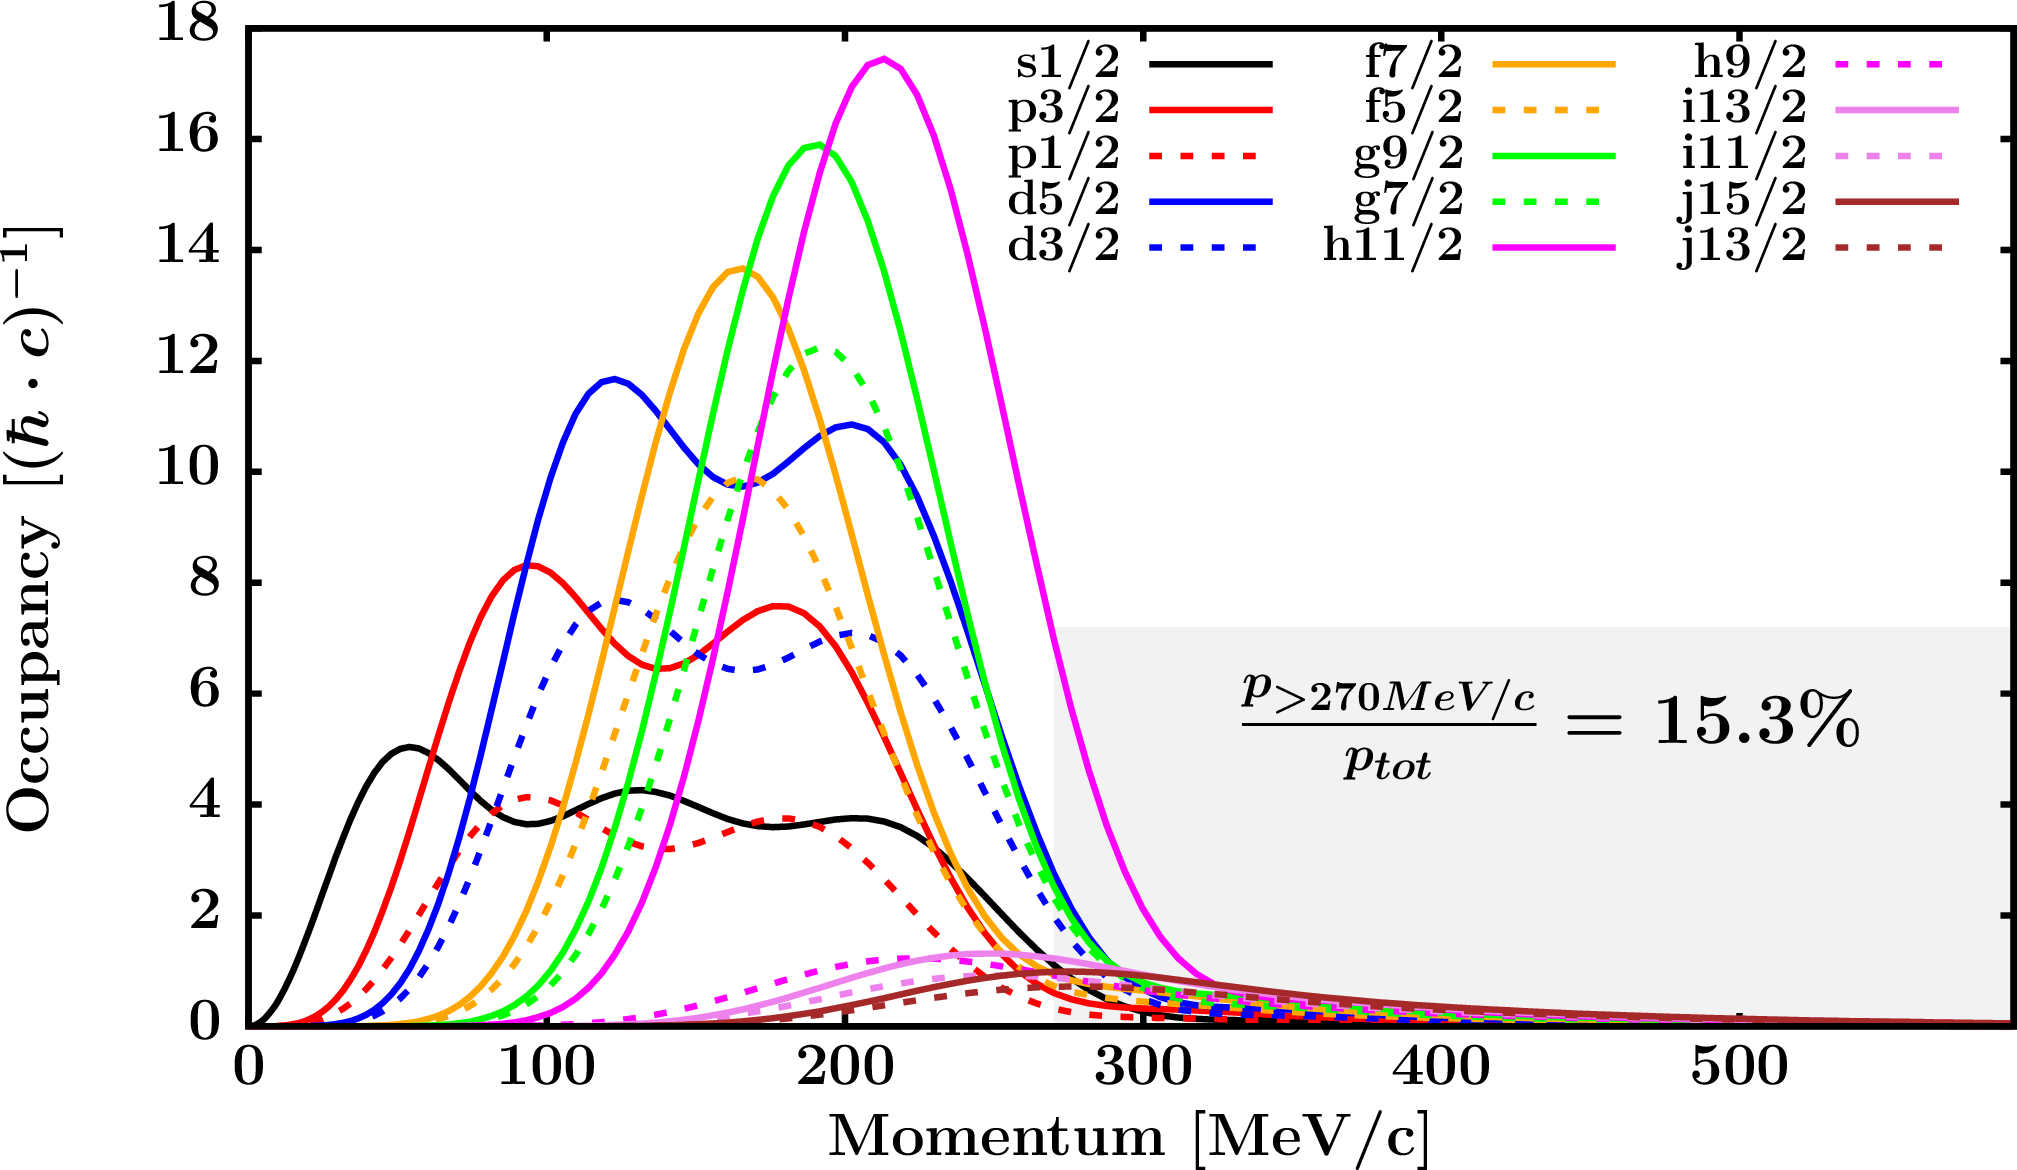
\includegraphics[width=0.75\textwidth]{figures/pb208_protonLJMomentumDistIntegral.png}
    \caption[Proton momentum distribution in \pbEight]
    {
        Integrated proton momentum distribution in \pbEight, as generated
        by our DOM fit. The fraction of proton density with
        momentum above 270 $\mega\electronvolt/\text{c}$ is listed.
    }
    \label{pb208ProtonMomentumDistInt}
    \vspace{16pt}
    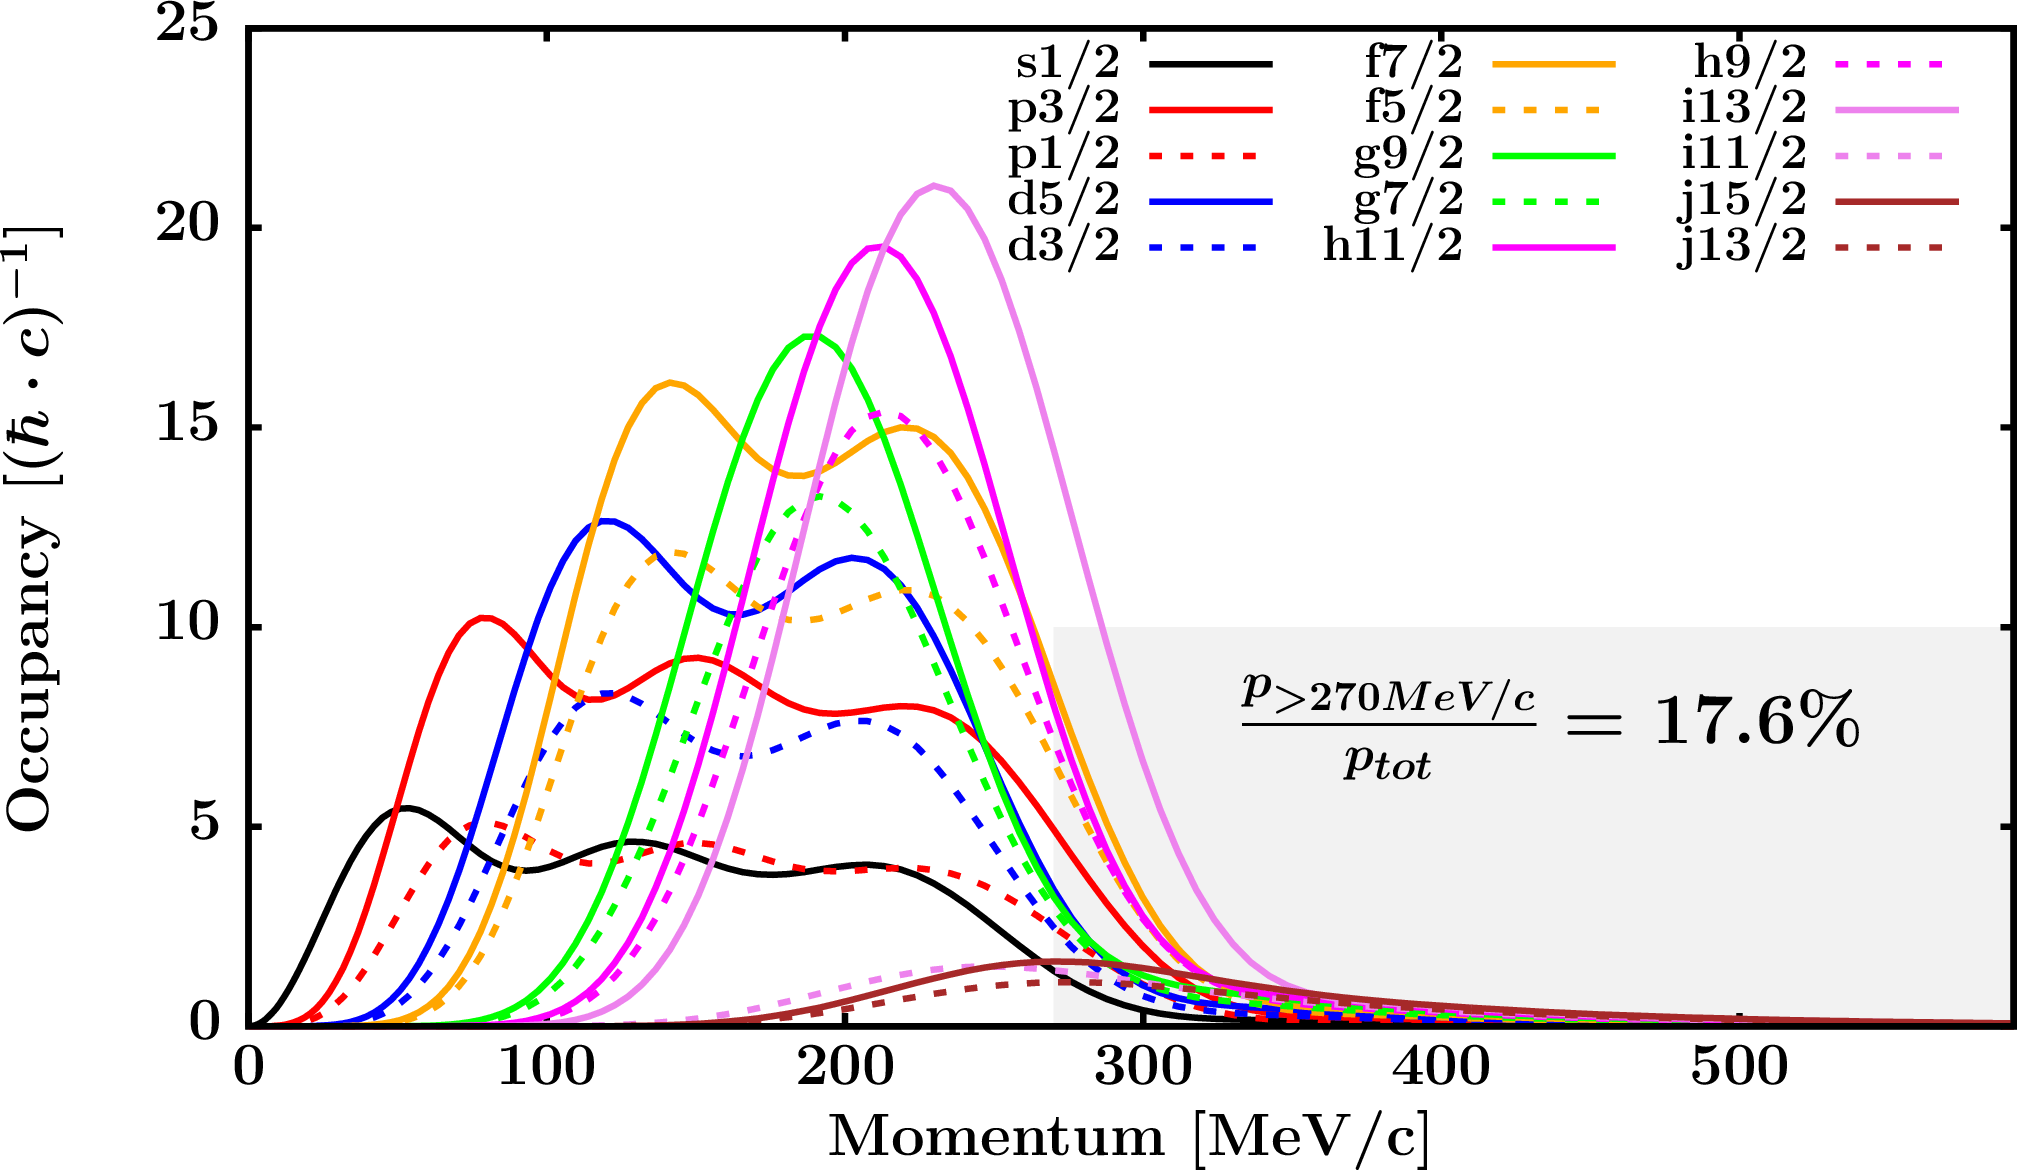
\includegraphics[width=0.75\textwidth]{figures/pb208_neutronLJMomentumDistIntegral.png}
    \caption[Neutron momentum distributions in \pbEight]
    {
        Integrated neutron momentum distribution in \pbEight, as generated
        by our DOM fit. The fraction of neutron density with
        momentum above 270 $\mega\electronvolt/\text{c}$ is listed.
    }
    \label{pb208NeutronMomentumDistInt}
\end{figure}

\begin{figure}[tb]
    \centering
    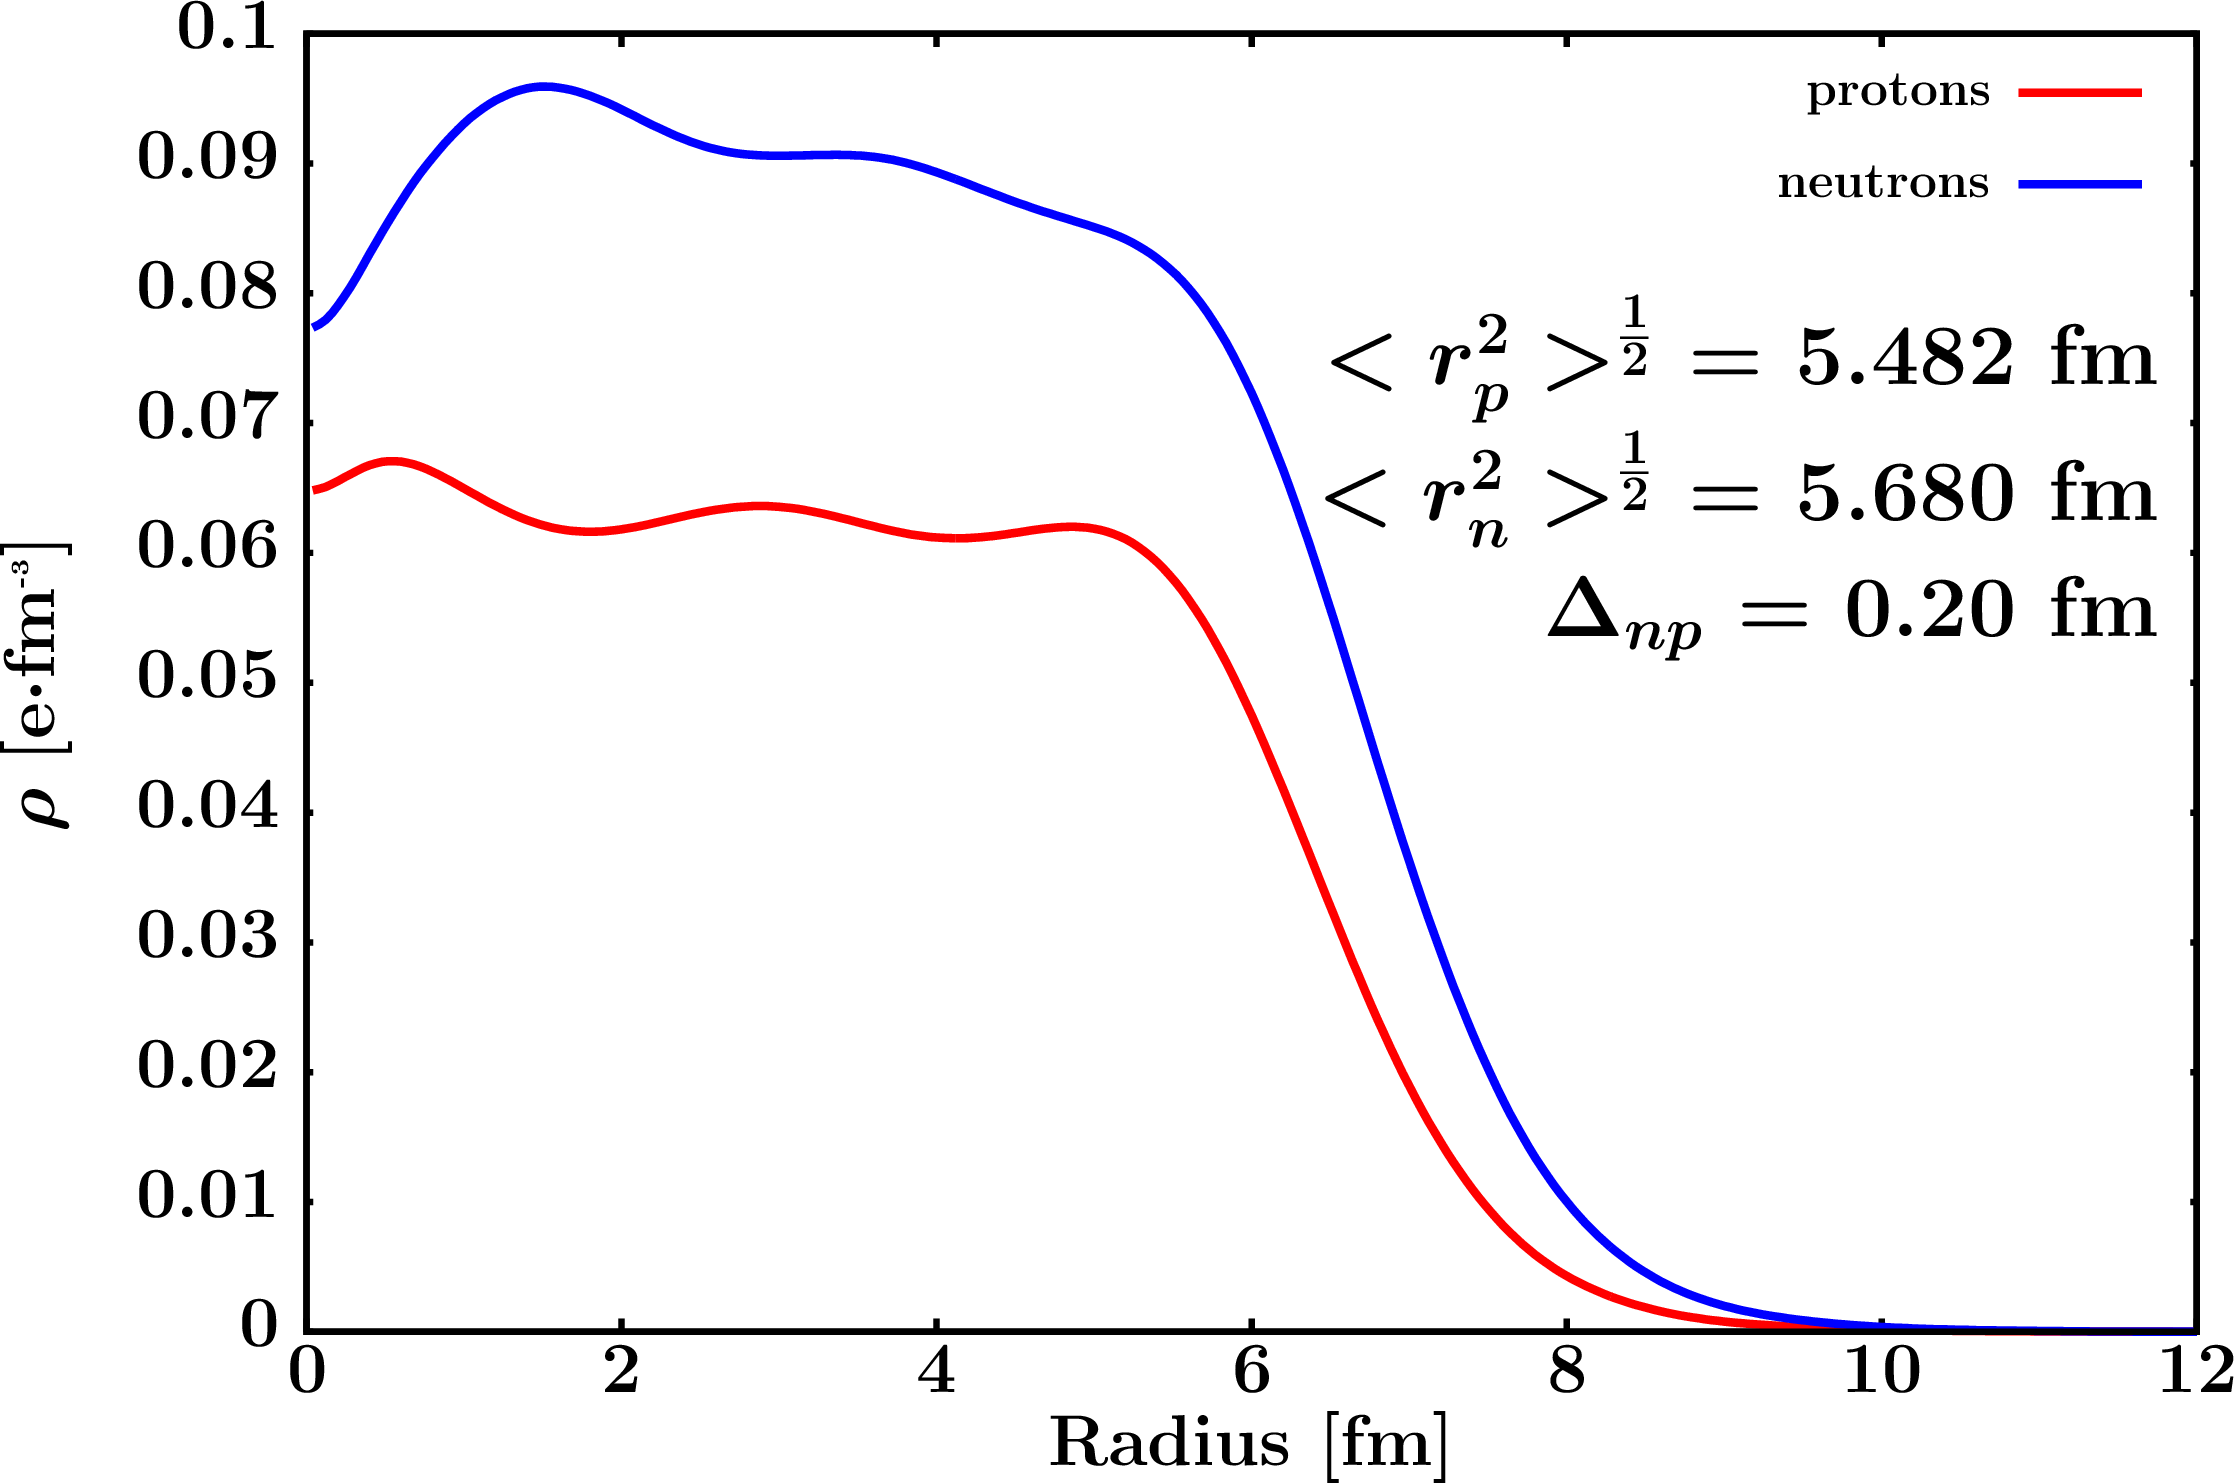
\includegraphics[width=\textwidth]{figures/pb208_matterDensity.png}
    \caption[Proton and neutron matter density distributions in \pbEight]
    {
        Proton and neutron point density distributions in \pbEight, as
        generated by our DOM fit. The RMS radii of the distributions and their
        difference (the neutron skin) are provided. The neutron skin of
        neutron-rich systems like \pbEight\ are expected to be strongly correlated
        with the size of the density-dependence of the symmetry energy, $L$.
    }
    \label{Pb208MatterDistribution}
\end{figure}

\section{General trends}
\subsection{Neutron skins sensitive to shell structure}
Table \ref{NeutronSkinsTable} presents the neutron skins we extracted from our
optimized DOM fits on all nuclei under study. As anticipated, both the total
degree of asymmetry and the specific shell structure affect the
calculated skins.
\\
\begin{table}[H]
    \centering
    \begin{tabular}{c c c c}
        \toprule
        Isotope & $\pi$ $r_{rms}$ [\femto\meter] & $\nu$ $r_{rms}$
        [\femto\meter] & $\Delta_{rms}$ [\femto\meter]\\
        \midrule
        \oSix & 2.685 & 2.661 & -0.024\\
        \oEight & 2.677  & 2.874 & 0.197\\

        \caForty & 3.470 & 3.414 & -0.056\\
        \caEight & 3.472 & 3.621 & 0.150\\

        \niEight & 3.738 & 3.733 & -0.005\\
        \niFour & 3.828 & 3.977 & 0.150\\

        \snTwelve 4.569 & 4.560 & -0.009\\
        \snFour & 4.608 & 4.780 & 0.170\\

        \pbEight & 5.482 & 5.680 & 0.200 \\
        \bottomrule
    \end{tabular}
    \caption[Neutron skins extracted from DOM analysis]
    {
        Neutron skins ($\Delta_{rms}$) extracted from DOM analysis. The skins are calculated as the difference between the
        proton and neutron point distribution root-mean-square (RMS) radii and thus do not include the
        nucleon-size form factor. All values are rounded, so the neutron skin reported
        in the last column may not exactly match the difference of proton and neutron
        RMS radii listed. The full calculated matter distributions for protons and
        neutrons for each nucleus are available in Appendix \ref{DOMVisualization}. 
    }
    \label{NeutronSkinsTable}
\end{table}

\subsection{Depletion, momentum content, and deep imaginary strength}
For over fifty years, (e,e'p) and (p,2p) measurements have shown that in real
nuclei, single-particle spectroscopic factors are significantly reduced both
near the Fermi surface and for deeply-bound subshells. Table
\ref{SpectroscopicFactorTable} shows
the spectroscopic factors for valence proton and neutron subshell
for each nucleus modeled in this work and indicates consistent reduction in 
spectroscopic factors by around 25-30\%, for valence subshells.
\begin{table}[H]
    \centering
    \begin{tabular}{c c c c c}
        \toprule
        \multirow{2}{*}{Isotope} & \multicolumn{2}{c}{Protons} &
        \multicolumn{2}{c}{Neutrons}\\
        \cmidrule(l{0.5em}r{0.5em}){2-3}
        \cmidrule(l{0.5em}r{0.5em}){4-5}
        & Level & SF & Level & SF\\
        \midrule
        \oSix & 0\pOne & 0.75 & 0\pOne & 0.75 \\
        \oEight & 0\pOne & 0.78 & 0\dFive & 0.76 \\

        \caForty & 0\dThree & 0.76 & 0\dThree & 0.76 \\
        \caEight & 1\sOne & 0.75 & 0\fSeven & 0.76 \\

        \niEight & 0\fSeven & 0.70 & 1\pThree & 0.71 \\
        \niFour & 0\fSeven & 0.74 & 1\pOne & 0.78 \\

        \snTwelve & 0\gNine & 0.70 & 1\dFive & 0.74 \\
        \snFour & 0\gNine & 0.72 & 0\hEleven & 0.76 \\

        \pbEight & 2\sOne & 0.67 & 1\fFive & 0.73 \\
        \bottomrule
    \end{tabular}
    \caption[Valence Spectroscopic Factors extracted from DOM analysis]
    {
        Spectroscopic factors for protons and neutrons in the valence
        subshell (e.g., $\pi$\pOne, $\nu$\dFive for \oEight) are listed for
        all nuclei considered in the present treatment. For some of the heavier
        systems with multiple, nearly-degenerate levels nears the Fermi surface
        (e.g., \snFour), we list only one representative level.
    }
    \label{SpectroscopicFactorTable}
\end{table}

When examined in momentum space,
the proton and neutron particle density distributions
are expected to show significant enhancement of nucleon density at higher momentum
than would be expected in an independent-particle shell model
\cite{RoheHabilitation}. The amount of this so-called
``high-momentum content'' has been investigated by knockout reactions
\cite{Rohe2004, RoheHabilitation} and shown to be significant even for very
light nuclei such as \cTwelve ($\approx10\% >
270 \mega\electronvolt/\text{c}$). Table \ref{HighMomentumContent} shows the
percentage of the proton and neutron densities with momentum above $270
\mega\electronvolt/\text{c}$ per our fits.
\begin{table}[tb]
    \caption[High-momentum content extracted from DOM analysis]
    {
        High-momentum content as extracted from DOM analysis. For protons and neutrons for each
        nucleus under study, the nucleon density distribution in momentum-space is calculated and
        the fraction of the density distribution above 270 \mega\electronvolt/c is
        tabulated. For comparison, \cite{Rohe2004} reported $\approx10\%$ high momentum content for
        \cTwelve. The full momentum-space matter distributions for protons and
        neutrons for each nucleus are available in Appendix \ref{DOMVisualization}. 
    }
    \label{HighMomentumContent}
    \centering
    \begin{tabular}{c c c c}
                \toprule
                Isotope & $\pi$ $p_{>270}$ [\%] & $\nu$ $p_{>270}$ [\%] & p/n Ratio\\
                \midrule
                \oSix & 15.3 & 15.7 & 0.97\\
                \oEight & 14.3 & 13.8 & 1.03\\

                \caForty & 13.9 & 14.6 & 0.95\\
                \caEight & 12.4 & 15.5 & 0.80\\

                \niEight & 12.3 & 14.8 & 0.83\\
                \niFour & 14.7 & 16.0 & 0.92\\

                \snTwelve & 14.9 & 18.7 & 0.80\\
                \snFour & 10.9 & 15.8 & 0.69\\

                \pbEight & 15.3 & 17.6 & 0.87\\
                \bottomrule
    \end{tabular}
\end{table}
The values we extract are roughly constant at around 12-15\% for protons and
15-18\% for neutrons. For
\snTwelve\ and \snFour\ where experimental coverage is most sparse, we
see deviations from the average, suggesting that our optimized fits require more
experimental data for a clearer picture. For the symmetric nuclei \oSix\ and \caForty,
we see that the neutron high-momentum
content is slightly larger than the proton high-momentum content, ostensibly
from a slight
broadening of the momentum distribution for neutron subshells compared to proton
subshells, which nudges more neutron density into the high-momentum regime.
\begin{figure}[tb]
    \centering
    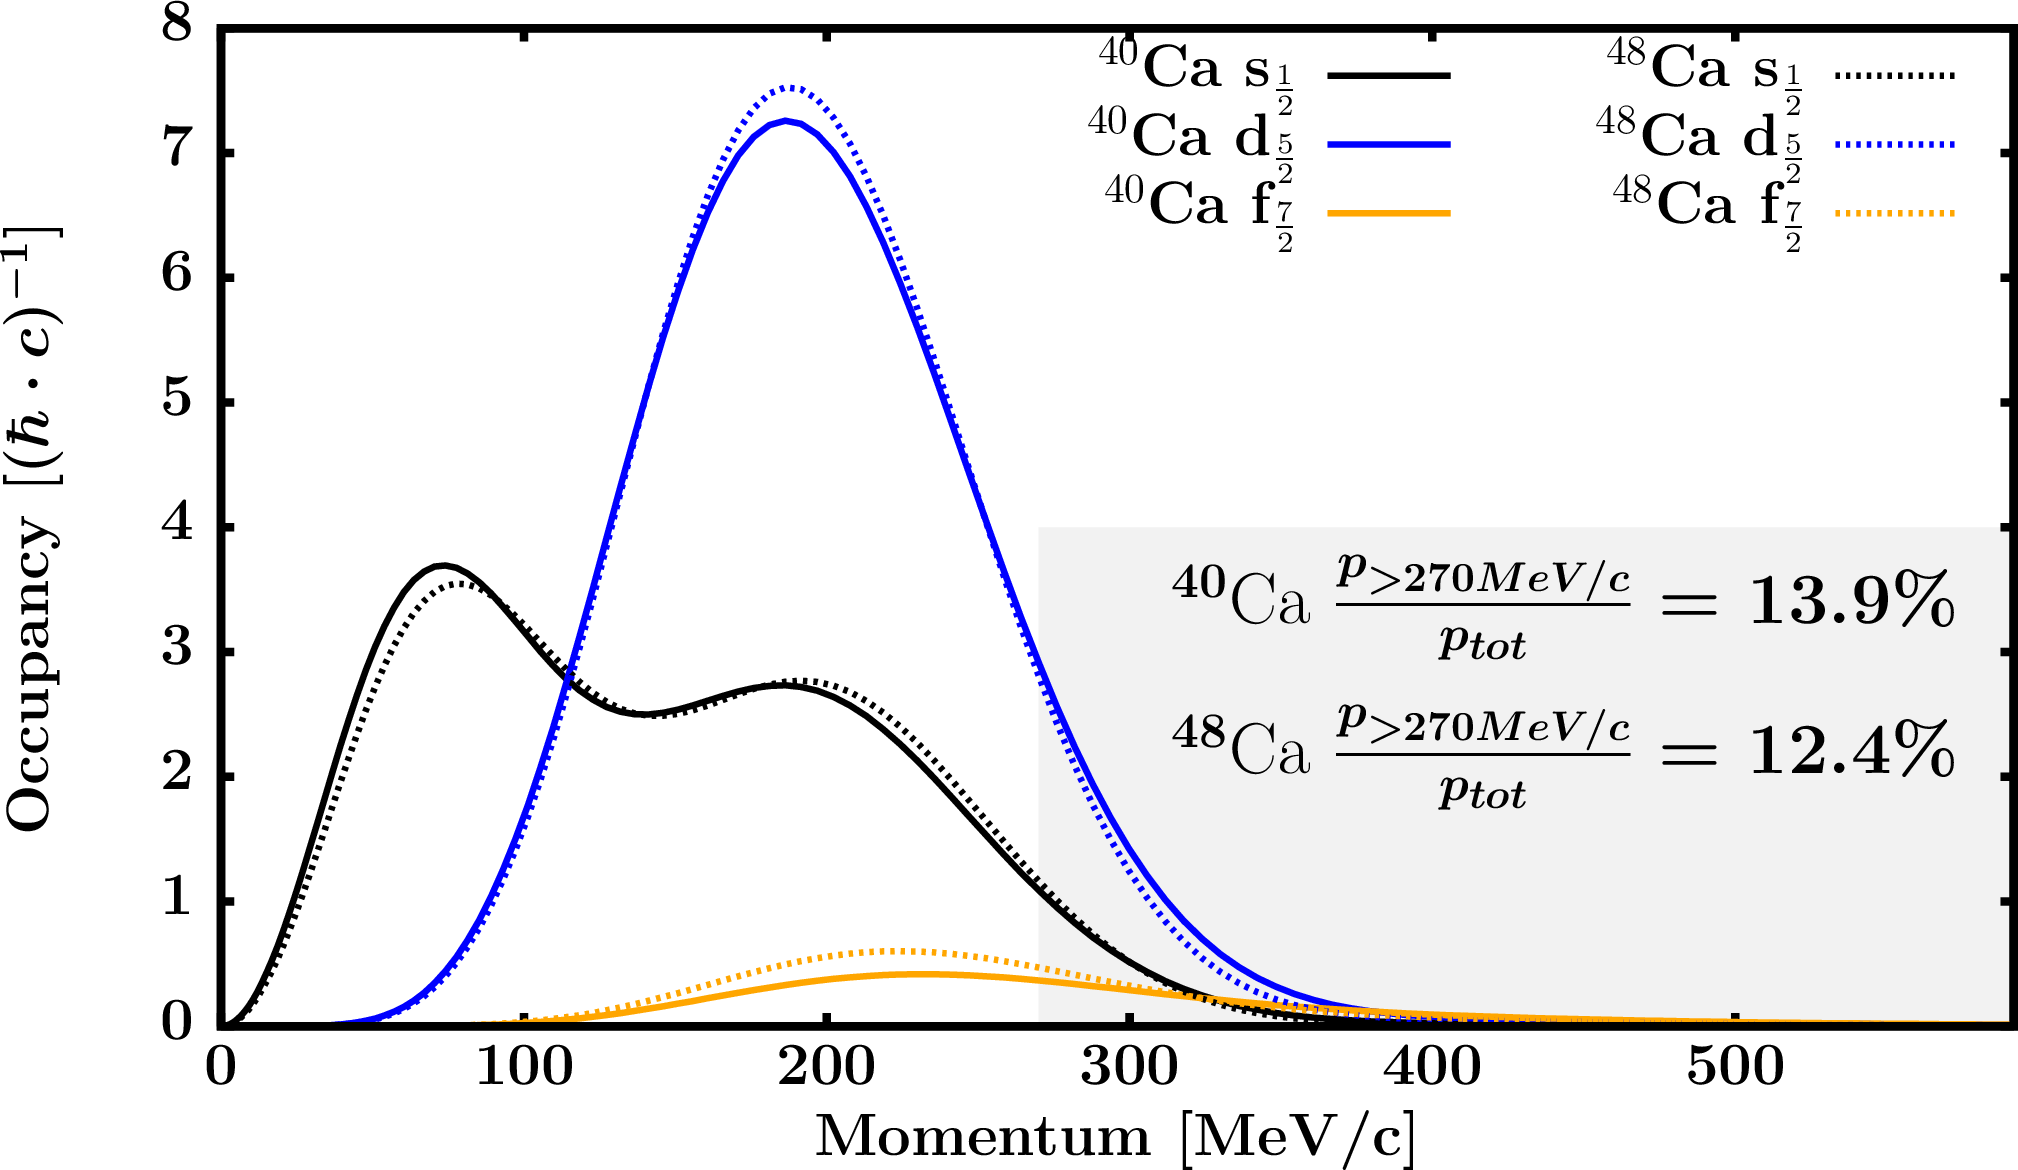
\includegraphics[width=0.85\textwidth]{figures/CaMomenta.png}
    \caption[Proton single-particle momentum distributions in \caAughtEight]
    {
        The proton \sOne, \dFive, and \fSeven\ momentum distributions for
        \caAughtEight\ are shown. Compared to \caForty, we see a slight reduction
        in the total \caEight\ proton high-momentum content over all subshells
        (the total fraction of protons with momentum above 270 $\mega\electronvolt/\text{c}$
        is listed in the gray box). This reduction is associated with a slight narrowing of the
        valence-region momentum distributions (e.g., \dFive\ and \fSeven)
        that are the dominant contributors to the total high-momentum fraction.
    }
    \label{CaMomenta}
\end{figure}

For highly asymmetric
nuclei (e.g., \snFour, \pbEight), we might expect that, \textit{all other things
being equal,} the minority nucleon species should have a
larger fraction of high-momentum content \cite{Subedi2008, Hen2012},
a consequence of the enhanced
short-range correlations experienced by the minority-species nucleons. At first
glance, our results appear to contradict this expectation: for example, in \caEight, we see a
\textit{reduction} in the percentage of proton
high-momentum content compared to \caForty\ (12.4\% for \caEight,
13.9\% for \caForty). However, a closer look at
the breakdown of momentum distributions by angular momenta (Fig.
\ref{CaMomenta}) shows that the story is more complicated. In going from
\caForty\ to \caEight, the nuclear potential widens and
the proton Fermi energy (and corresponding Fermi momentum) drops considerably,
by almost 10 \mega\electronvolt. Per our fit, the first lobe
of the proton \sOne\ momentum distribution appears to shift toward higher
momentum slightly, but the second lobe (corresponding to the proton 1\sOne
level) narrows slightly. More importantly, the subshells that contribute
the most to the proton high-momentum content
(e.g., the proton \dFive\ and \fSeven) are also reduced in width, lessening the
overall high-momentum fraction. It is plausible that the narrowing of the
momentum-space peaks is due to the widening of the proton potential
from the eight extra neutrons in \caEight, but it also may indicate that our
parameterization is insufficiently flexible to reproduce the true potential. In any
case, our results suggest that to connect
short-range correlations with increased high-momentum content,
a fixed momentum threshold (e.g., 270 $\mega\electronvolt/\text{c}$) may not be
useful for comparing nuclei and a more nuanced treatment may be needed.
Of course, additional experimental data to constrain the deep negative-energy
regime for \caEight, especially for neutrons, would be quite valuable.

The deep negative-energy realm is perhaps the most challenging sector for our fit,
as our only direct constraint is the experimental binding energy. Because the
binding energy does not differentiate between protons and neutrons, we have
very limited sensitivity to the isovector-dependence of the potential in
this area. As a result, the relative high-momentum content between protons and
neutrons that we extract can only be taken qualitatively, though the absolute
high-momentum content values from our fits are in general agreement with the
results of \cite{Rohe2004, RoheHabilitation}.

\subsection{Overestimation of RMS charge radius}
The charge density distributions extracted from our fits showed a slight
excess of charge density on the extreme tail of the distributions (e.g., above 5 
\femto\meter\ for \caForty). As the RMS charge radius is most sensitive to
contributions from the tail, this excess led to chronic overestimation of the RMS
charge radius of roughly 0.05-0.10 \femto\meter\ across nuclei.
We found that density in the extreme tail of the matter distributions was very
sensitive to the amount of imaginary strength just below the Fermi energy
($W_{sur}^{-}$); in fits with a high weight for the RMS charge radius,
$W_{sur}^{-}$ would tend toward zero or even cross into negative territory,
which is unphysical. Especially in the lighter systems we studied, our fits routinely
moved all the negative-energy imaginary strength into $W_{vol}^{-}$.
We had no difficulties fitting $W_{sur}^{+}$, largely due to the
availability of proton \rxn\ and neutron \tot\ data from 20-50 MeV.
Interestingly, the volume
integral of the imaginary strength (an integration over the
radial form factors) of our optimized fits shows the imaginary potential to be largely symmetric
about the Fermi energy within roughly 30 MeV (see Fig. \ref{Ca40ProtonVolumeIntegral}),
in keeping with the expectations of \cite{Mahaux1991} and many other theoretical
treatments. Whether the partitioning
of the negative-energy imaginary strength into $W_{vol}^{-}$ over $W_{sur}^{-}$
has real significance is unclear, but it suggests that subsequent 
analyses may need more specialized treatment in the near-surface negative-energy
regime.

Practically speaking, because the nuclear surface and volume overlap
significantly in light systems like \oSix, we did not expect to see a unique best-fit for the
negative-energy parameters. In real nuclei near the Fermi surface,
imaginary strength should vary rapidly due to the discrete resonance structure of
the nucleus. In this region, the optical potential corresponds quite poorly
with this reality as it can only represent a smooth average. With these
considerations in mind, it is perhaps
not surprising that we had trouble getting
the negative-energy surface parameters under control. In the end, for
\oSixEight\ we fixed $W_{sur}^{-}$ to zero for
the final optimizations to avoid numerical problems and prevent any
unphysical imaginary parameter values. In our fits, the
$W_{vol}^{-}$ term had no trouble providing imaginary strength where it was
needed to recover correct particle numbers, charge density distributions, and,
to some extent, binding energies.

It should be noted that while we produce RMS charge radii that are a tad high
compared to experimental measurements, we had good success recovering the shape
of the full charge density distribution profiles. As the neutron skin is the
\textit{difference} between proton and neutron matter radii, any systematic
issues that affect both the neutron and proton matter distributions should have
only a small effect on our neutron skin values.
\afterpage{\clearpage}
